\expandafter\ifx\csname MasterFile\endcsname\relax
	\def\SubFile{hoge}
  \documentclass[a4j,12pt,twoside,openany]{jreport}
%\nofiles %tocファイルを更新させない
%\documentclass[12pt,a4j,twoside,openany]{jsbook}
\usepackage[dvipdfmx]{graphicx}
\usepackage{../dspc} % ベースラインスキップの指定
\usepackage{../slashbox} % 表に斜線を入れる
%\usepackage{../mediabb}
\usepackage{fancyvrb} % Verbatim環境
\usepackage{fancyhdr} % Headerの下線付き章見出し
\usepackage{here} % float[H]
\usepackage{multirow}
\usepackage{hhline} % 表の罫線の角を美しくする
\usepackage{amsmath} %コレがないとcasesが動かない
\usepackage{amsfonts} % 数学用フォント
\usepackage{bm} % 数式環境での bold
\usepackage{algorithm}
\usepackage{algorithmicx}
\usepackage[noend]{algpseudocode}%\procedureはここに含まれる
\usepackage[flushleft]{threeparttable} % 脚注付きテーブル
\usepackage{enumitem}
\usepackage{comment}
\usepackage{fancybox}
%\usepackage{csvsimple,booktabs,siunitx}
%\usepackage{filecontents}
\usepackage{ulinej}


\setlength{\evensidemargin}{5pt}
\setlength{\oddsidemargin}{40pt}
%\setlength{\headheight}{16.5pt}
%%\setlength{\headheight}{30pt}
\setcounter{secnumdepth}{3}
\setlist[description]{leftmargin=2\parindent,labelindent=\parindent}

\makeatletter
\def\@makechapterhead#1{%
	\vspace*{50\p@}%
	{
		\parindent \z@ \raggedright \normalfont
		\ifnum \c@secnumdepth >\m@ne
		% \if@mainmatter
			\huge\bfseries\@chapapp\thechapter\@chappos
			\par\nobreak
			\vskip 20\p@
		% \fi
		\fi
		\interlinepenalty\@M
		\Huge\bfseries #1\par\nobreak
		\vskip 40\p@
	}
}

%新しいコマンド定義
\newcounter{linenumber}
\newenvironment{listing}{%
  \begin{list}{%
    \small\arabic{linenumber}:}{%
      \usecounter{linenumber}%
      \setlength{\baselineskip}{18pt}%
      \setlength{\itemsep}{0pt}%
      \setlength{\parsep}{0pt}}}%
 {\end{list}}
\newcommand{\figcaption}[1]{\def\@captype{figure}\caption{#1}}
\newcommand{\tblcaption}[1]{\def\@captype{table}\caption{#1}}
\newcommand{\norm}[1]{\left\| #1 \right\|}
\newcommand{\cc}[1]{\multicolumn{1}{|c|}{#1}}
\newcommand{\circled}[1]{\raisebox{.5pt}{\textcircled{\raisebox{-.9pt} {#1}}}}
\newcommand{\specialcell}[2][c]{%
  \begin{tabular}[#1]{@{}c@{}}#2\end{tabular}}
\makeatother
%===============================================================================
\expandafter\ifx\csname SubFile\endcsname\relax
\begin{document}
\def\MasterFile{hoge}
%-------------------------------------------------------------------------------
%\maketitle
\thispagestyle{empty}
\documentclass[a4j,12pt]{jarticle}
% 外表紙

% 題名
\def\title{降水量予測のための\\Sequence-to-Sequenceモデルに基づく\\マルチモーダル学習}
% 著者
\def\author{林 政行}
% 入学年度(平成)
\def\year{24}
% 学籍番号
\def\number{24115113}
% 指導教官
\def\kyoukan{伊藤孝行}
% 指導教官役職
\def\kyoukanrank{教授}
% 提出日
\def\teisyutubi{平成28年2月8日}

\begin{document}
\pagestyle{empty}
\baselineskip=18pt

\begin{center}

\vspace*{2cm}

{\huge \textbf{卒業論文}}

\vspace*{3cm}

%\vrule width 10cm height 1pt depth 0pt



%(題目)
%\vspace{5pt}
%\hrule height 3pt
%\vspace{1zh}

\vrule width 6.25cm height 6pt depth -2pt
\makebox[1.5cm]{(題目)}
\vrule width 6.25cm height 6pt depth -2pt

{\LARGE {\title}}

\vspace{1zh}
%{\large {\subtitle}}
%\hrule height 3pt
\vrule width 14cm height 4pt depth 0pt

\vspace*{1cm}

指導教員 {\large {\kyoukan}} {\kyoukanrank}

%\vspace*{5cm}
\vfill

{\large 名古屋工業大学 情報工学科}

{\large 平成{\year}年度 入学 ({\number})}

\vspace*{1cm}

%{\huge\mc {\author}}

\underline{(氏名)\hspace{3zw}{\huge\mc {\author}}\hspace{3zw}}

\vspace*{1cm}

({\teisyutubi}提出)

\vspace{2cm}
\end{center}

\end{document}
\begin{titlepage}

% 題名
\def\title{分散表現を用いた\\話題変化判定}
% 補助題名
\def\subtitle{卒業論文}
% 著者
\def\author{芳野 魁}
% 入学年度(平成)
\def\year{29}
% 学籍番号
\def\number{26115162}
% 指導教官
\def\kyoukan{伊藤 孝行}
% 指導教官役職
\def\kyoukanrank{教授}
% 提出日
\def\teisyutubi{平成29年9月19日}

\pagestyle{empty}

\begin{center}

\vspace*{20mm}
{\Large\mc 平成29年度 \hspace{7mm} 卒 業 論 文}
\vspace{15mm}

%\setlength{\unitlength}{1mm}
\begin{picture}(100,60)
  \put(0,0){\makebox(100,60){\huge\bf\shortstack{\title}}}
\end{picture}
\\
%\begin{picture}(100,5)
%  \put(0,0){\makebox(100,5){\Large\bf\shortstack{\subtitle}}}
%\end{picture}
\end{center}
\vspace{10mm}
\begin{flushright}
\begin{tabular}{ll}
{\large 提出日} & {\large {\teisyutubi}} \\
{\large 所属}  & {\large 名古屋工業大学 情報工学科} \\
{\large 指導教員} & {\large {\kyoukan} {\kyoukanrank}} \\
 & \\
{\large 入学年度} & {\large 平成{\year}年度入学}\\
{\large 学籍番号} &{\large {\number}} \\
 & \\
%{\large 氏名} & {\huge {\author}}
{\large 氏名} & {\huge\mc {\author}}
\end{tabular}
\end{flushright}

\end{titlepage}

%\addcontentsline{toc}{chapter}{表紙}
\thispagestyle{empty}
\mbox{}\newpage
%===============================================================================
%\frontmatter
%===============================================================================
%\mainmatter
%-------------------------------------------------------------------------------
\pagenumbering{arabic}
\cleardoublepage
\expandafter\ifx\csname MasterFile\endcsname\relax
\def\SubFile{hoge}
\documentclass[a4j,12pt,twoside,openany]{jreport}
%\nofiles %tocファイルを更新させない
%\documentclass[12pt,a4j,twoside,openany]{jsbook}
\usepackage[dvipdfmx]{graphicx}
\usepackage{../dspc} % ベースラインスキップの指定
\usepackage{../slashbox} % 表に斜線を入れる
%\usepackage{../mediabb}
\usepackage{fancyvrb} % Verbatim環境
\usepackage{fancyhdr} % Headerの下線付き章見出し
\usepackage{here} % float[H]
\usepackage{multirow}
\usepackage{hhline} % 表の罫線の角を美しくする
\usepackage{amsmath} %コレがないとcasesが動かない
\usepackage{amsfonts} % 数学用フォント
\usepackage{bm} % 数式環境での bold
\usepackage{algorithm}
\usepackage{algorithmicx}
\usepackage[noend]{algpseudocode}%\procedureはここに含まれる
\usepackage[flushleft]{threeparttable} % 脚注付きテーブル
\usepackage{enumitem}
\usepackage{comment}
\usepackage{fancybox}
%\usepackage{csvsimple,booktabs,siunitx}
%\usepackage{filecontents}
\usepackage{ulinej}


\setlength{\evensidemargin}{5pt}
\setlength{\oddsidemargin}{40pt}
%\setlength{\headheight}{16.5pt}
%%\setlength{\headheight}{30pt}
\setcounter{secnumdepth}{3}
\setlist[description]{leftmargin=2\parindent,labelindent=\parindent}

\makeatletter
\def\@makechapterhead#1{%
	\vspace*{50\p@}%
	{
		\parindent \z@ \raggedright \normalfont
		\ifnum \c@secnumdepth >\m@ne
		% \if@mainmatter
			\huge\bfseries\@chapapp\thechapter\@chappos
			\par\nobreak
			\vskip 20\p@
		% \fi
		\fi
		\interlinepenalty\@M
		\Huge\bfseries #1\par\nobreak
		\vskip 40\p@
	}
}

%新しいコマンド定義
\newcounter{linenumber}
\newenvironment{listing}{%
  \begin{list}{%
    \small\arabic{linenumber}:}{%
      \usecounter{linenumber}%
      \setlength{\baselineskip}{18pt}%
      \setlength{\itemsep}{0pt}%
      \setlength{\parsep}{0pt}}}%
 {\end{list}}
\newcommand{\figcaption}[1]{\def\@captype{figure}\caption{#1}}
\newcommand{\tblcaption}[1]{\def\@captype{table}\caption{#1}}
\newcommand{\norm}[1]{\left\| #1 \right\|}
\newcommand{\cc}[1]{\multicolumn{1}{|c|}{#1}}
\newcommand{\circled}[1]{\raisebox{.5pt}{\textcircled{\raisebox{-.9pt} {#1}}}}
\newcommand{\specialcell}[2][c]{%
  \begin{tabular}[#1]{@{}c@{}}#2\end{tabular}}
\makeatother
%===============================================================================
\expandafter\ifx\csname SubFile\endcsname\relax
\begin{document}
\def\MasterFile{hoge}
%-------------------------------------------------------------------------------
%\maketitle
\thispagestyle{empty}
\input{../hyoushi/hyoushi}
\input{../hyoushi/title}
%\addcontentsline{toc}{chapter}{表紙}
\thispagestyle{empty}
\mbox{}\newpage
%===============================================================================
%\frontmatter
%===============================================================================
%\mainmatter
%-------------------------------------------------------------------------------
\pagenumbering{arabic}
\cleardoublepage
\input{../0.Abstract/chapter}
%-------------------------------------------------------------------------------
\clearpage
\addcontentsline{toc}{chapter}{目次}
\tableofcontents

\clearpage
\addcontentsline{toc}{chapter}{図目次}
\listoffigures

\clearpage
\addcontentsline{toc}{chapter}{表目次}
\listoftables

%-------------------------------------------------------------------------------

%=====================
\pagestyle{fancy} % Headerをつける
\renewcommand{\sectionmark}[1]{\markright{\thesection\ \ \ #1}}
\renewcommand{\chaptermark}[1]{\markboth{#1}{}}
\lhead{}
\chead{}
\lfoot{}
\rfoot{}%-------------------------------------------------------------------------------
\input{../1.Introduction/chapter}
%-------------------------------------------------------------------------------
\input{../2.Related_Work/chapter}
%-------------------------------------------------------------------------------
\input{../3.The_Model/chapter}
%-------------------------------------------------------------------------------
\input{../4.Implementation/chapter}
%-------------------------------------------------------------------------------
\input{../5.Experiments/chapter}
%-------------------------------------------------------------------------------
\input{../6.Conclusion/chapter}

%===============================================================================
\pagestyle{plain}
%-------------------------------------------------------------------------------
\input{../7.Acknowledgement/chapter} %謝辞
%-------------------------------------------------------------------------------
\def\BibFile{../Bibliograhoy/database2}
\input{../Bibliography/chapter} %参考文献
% %===============================================================================
\appendix
\input{../A.Mypaper/chapter} % 投稿論文リスト
\input{../B.SIG-CCI2/chapter} %
\input{../C.IPSJ80/chapter} %
\input{../D.TopicGraph/chapter} %
%===============================================================================
\end{document}\input{../../../../../../../Downloads/2章.docx}

\fi

\begin{document}
\fi
%-------------------------------------------------------------------------------
\cleardoublepage
\chapter*{論文要旨}\addcontentsline{toc}{chapter}{論文要旨}
近年,Web上での大規模な議論活動が活発になっているが,現在一般的に使われている "2ちゃんねる" や "Twitter" といったシステムでは整理や収束を行うことが困難である.困難である原因として,議論の管理を行う者がいないことが挙げられる.
議論を収束させるには議論のマネジメントを行う人物が必要である.
%
大規模意見集約システムCOLLAGREEではファシリテーターと呼ばれる人物が議論のマネジメントを行っている.
しかし,ファシリテーターは人間であり,長時間に渡って大人数での議論の動向をマネジメントし続けるのは困難である.
%
COLLAGREEで大規模な議論を収束させるためには,ファシリテーターが必要な時にだけ画面を見るようにして画面に向き合う時間を減らす工夫があることが望ましい.ファシリテーターが画面を見るべきタイミングは議論の話題が変化したときである.以前の議論の内容から外れた発言がされた時,ファシリテーターが適切に発言することで,脱線や炎上を避けて議論を収束させることができる.
すなわち,ファシリテーターの代わりに自動的に議論中の話題の変化を事前に判定することが求められている.
%
現在,COLLAGREE上で使用されている議論支援システムは投稿支援システムと議論可視化システムの2つに大別できる.
投稿支援システムはポイント機能やファシリテーションフレーズ簡易投稿機能のように,ユーザーが投稿をする際に何らかの補助やリアクションを行う.現行の機能では選択肢の提示に留まっており,作業量を減らすことには繋がりにくい。
一方,議論可視化システムは議論ツリーやキーワード抽出のように,ユーザーにスレッドとは異なる議論の見方を提供する.現行の機能では議論を見やすくすることに重点が置かれており,議論の把握の助けにはなるが画面に向き合う時間を減らすことにはなりにくい.むしろ,作業量を増やすことになり得る機能もある.
\begin{comment}
ポイント機能(ユーザの議論行動を活性化)-1
ファシリテーションフレーズ簡易投稿機能-1
議論ツリー-2
1文の要約,スレッドの要約,クラスタリング,返信意見の極性判定-2
ファシリテーションスタンプ-1
キーワード抽出-2
いいね機能-1
いいねランキング-2
投票機能-1
議論フェーズ機能-2
1-意見を出す、投稿をする際に補助や選択肢、リアクションを与える
2-議論の別の見方を提供する
\end{comment}
%
近年,自然言語処理の分野において分散表現が多くの研究で使われており,機械翻訳を始めとする単語の意味が重要となる分野で精度の向上が確認されている.分散表現を用いることで,人間に近い精度で話題の変化を観測することが可能となる.
%
以上のような背景を踏まえて,分散表現を用いて,話題の変化を観測し,話題の変化が確認された時にファシリテーターに伝えることが望ましい.
話題の変化の観測は,発言中に現れる単語の関連度合いの計算と見なすことができる.
分散表現を用いることで単語間の類似度を求めることができる,値が大きいほど単語がそれぞれ類似した実数ベクトルであることを表す.単語Aと単語Bの実数ベクトルが類似しているとは,単語Aと共に使われることの多い単語と単語Bと共に使われることの多い単語が多く共通していることを示す.故に,分散表現を使って単語の関連度を計算することができる.
%
発言文から単語を選ぶ際には自動要約を用いる.発言文から重要でない単語を取り除くことで関連度の計算の精度を高めることが可能となる.
%
本論文では,分散表現を用いて議論中での発言に含まれる単語の関連度を計算し,話題の変化を観測する手法を提案する.
%
提案手法は,既存の抽出的要約手法を用いて選ばれた単語の関連度を計算する手法,Seq2Seqによる生成的要約を用いて生成された単語の関連度を計算する手法,オントロジーを用いて求められた単語の関連度を計算する手法の3つである.
提案した3つの手法により,議論中の話題の変化の観測の評価実験を行い,各手法の評価を行う.
評価実験によって,提案手法を用いることで人間の代わりに自動的に話題の変化を観測できることを確認する.
%
 \begin{comment}
大規模な議論では意見を共有することは可能であるが,議論を整理させることや収束させることは難しい.以上から大規模意見集約システムCOLLAGREEが開発された.本システムではWeb上で適切に大規模な議論を行うことができるように議論をマネジメントするファシリテーターを導入した.
過去の実験ではファシリテーターの存在が議論の集約に大きな役割を果たしていることが認識されており,大規模な議論のためにファシリテータは必要である.しかし,議論の規模に伴って議論時間が長くなる傾向があり,同時にファシリテーターは常に議論の動向を見続ける必要がある.故に,議論の規模が大きくなればなるほどファシリテーターは長時間かつ大規模な議論の動向の監視によって大きな負担がかかる.大規模な議論が増加する傾向を踏まえるとファシリテーターにかかる負担を軽減する支援が必要となることは明白である.
また,近年自然言語処理の分野において分散表現が多くの研究で使われており,機械翻訳を始めとする複数の分野で精度の向上が確認されている.まだ適応されていない分野でも結果の向上が期待できる.
従って,本研究では負担軽減の1つとして分散表現を用いて議論中での話題の変化を人間の代わりに検知することでファシリテーターの負担を軽減することを目指す.
-----------------

\end{comment}
%-------------------------------------------------------------------------------
\expandafter\ifx\csname MasterFile\endcsname\relax
\end{document}
\fi

%-------------------------------------------------------------------------------
\clearpage
\addcontentsline{toc}{chapter}{目次}
\tableofcontents

\clearpage
\addcontentsline{toc}{chapter}{図目次}
\listoffigures

\clearpage
\addcontentsline{toc}{chapter}{表目次}
\listoftables

%-------------------------------------------------------------------------------

%=====================
\pagestyle{fancy} % Headerをつける
\renewcommand{\sectionmark}[1]{\markright{\thesection\ \ \ #1}}
\renewcommand{\chaptermark}[1]{\markboth{#1}{}}
\lhead{}
\chead{}
\lfoot{}
\rfoot{}%-------------------------------------------------------------------------------
\expandafter\ifx\csname MasterFile\endcsname\relax
\def\SubFile{hoge}
\documentclass[a4j,12pt,twoside,openany]{jreport}
%\nofiles %tocファイルを更新させない
%\documentclass[12pt,a4j,twoside,openany]{jsbook}
\usepackage[dvipdfmx]{graphicx}
\usepackage{../dspc} % ベースラインスキップの指定
\usepackage{../slashbox} % 表に斜線を入れる
%\usepackage{../mediabb}
\usepackage{fancyvrb} % Verbatim環境
\usepackage{fancyhdr} % Headerの下線付き章見出し
\usepackage{here} % float[H]
\usepackage{multirow}
\usepackage{hhline} % 表の罫線の角を美しくする
\usepackage{amsmath} %コレがないとcasesが動かない
\usepackage{amsfonts} % 数学用フォント
\usepackage{bm} % 数式環境での bold
\usepackage{algorithm}
\usepackage{algorithmicx}
\usepackage[noend]{algpseudocode}%\procedureはここに含まれる
\usepackage[flushleft]{threeparttable} % 脚注付きテーブル
\usepackage{enumitem}
\usepackage{comment}
\usepackage{fancybox}
%\usepackage{csvsimple,booktabs,siunitx}
%\usepackage{filecontents}
\usepackage{ulinej}


\setlength{\evensidemargin}{5pt}
\setlength{\oddsidemargin}{40pt}
%\setlength{\headheight}{16.5pt}
%%\setlength{\headheight}{30pt}
\setcounter{secnumdepth}{3}
\setlist[description]{leftmargin=2\parindent,labelindent=\parindent}

\makeatletter
\def\@makechapterhead#1{%
	\vspace*{50\p@}%
	{
		\parindent \z@ \raggedright \normalfont
		\ifnum \c@secnumdepth >\m@ne
		% \if@mainmatter
			\huge\bfseries\@chapapp\thechapter\@chappos
			\par\nobreak
			\vskip 20\p@
		% \fi
		\fi
		\interlinepenalty\@M
		\Huge\bfseries #1\par\nobreak
		\vskip 40\p@
	}
}

%新しいコマンド定義
\newcounter{linenumber}
\newenvironment{listing}{%
  \begin{list}{%
    \small\arabic{linenumber}:}{%
      \usecounter{linenumber}%
      \setlength{\baselineskip}{18pt}%
      \setlength{\itemsep}{0pt}%
      \setlength{\parsep}{0pt}}}%
 {\end{list}}
\newcommand{\figcaption}[1]{\def\@captype{figure}\caption{#1}}
\newcommand{\tblcaption}[1]{\def\@captype{table}\caption{#1}}
\newcommand{\norm}[1]{\left\| #1 \right\|}
\newcommand{\cc}[1]{\multicolumn{1}{|c|}{#1}}
\newcommand{\circled}[1]{\raisebox{.5pt}{\textcircled{\raisebox{-.9pt} {#1}}}}
\newcommand{\specialcell}[2][c]{%
  \begin{tabular}[#1]{@{}c@{}}#2\end{tabular}}
\makeatother
%===============================================================================
\expandafter\ifx\csname SubFile\endcsname\relax
\begin{document}
\def\MasterFile{hoge}
%-------------------------------------------------------------------------------
%\maketitle
\thispagestyle{empty}
\input{../hyoushi/hyoushi}
\input{../hyoushi/title}
%\addcontentsline{toc}{chapter}{表紙}
\thispagestyle{empty}
\mbox{}\newpage
%===============================================================================
%\frontmatter
%===============================================================================
%\mainmatter
%-------------------------------------------------------------------------------
\pagenumbering{arabic}
\cleardoublepage
\input{../0.Abstract/chapter}
%-------------------------------------------------------------------------------
\clearpage
\addcontentsline{toc}{chapter}{目次}
\tableofcontents

\clearpage
\addcontentsline{toc}{chapter}{図目次}
\listoffigures

\clearpage
\addcontentsline{toc}{chapter}{表目次}
\listoftables

%-------------------------------------------------------------------------------

%=====================
\pagestyle{fancy} % Headerをつける
\renewcommand{\sectionmark}[1]{\markright{\thesection\ \ \ #1}}
\renewcommand{\chaptermark}[1]{\markboth{#1}{}}
\lhead{}
\chead{}
\lfoot{}
\rfoot{}%-------------------------------------------------------------------------------
\input{../1.Introduction/chapter}
%-------------------------------------------------------------------------------
\input{../2.Related_Work/chapter}
%-------------------------------------------------------------------------------
\input{../3.The_Model/chapter}
%-------------------------------------------------------------------------------
\input{../4.Implementation/chapter}
%-------------------------------------------------------------------------------
\input{../5.Experiments/chapter}
%-------------------------------------------------------------------------------
\input{../6.Conclusion/chapter}

%===============================================================================
\pagestyle{plain}
%-------------------------------------------------------------------------------
\input{../7.Acknowledgement/chapter} %謝辞
%-------------------------------------------------------------------------------
\def\BibFile{../Bibliograhoy/database2}
\input{../Bibliography/chapter} %参考文献
% %===============================================================================
\appendix
\input{../A.Mypaper/chapter} % 投稿論文リスト
\input{../B.SIG-CCI2/chapter} %
\input{../C.IPSJ80/chapter} %
\input{../D.TopicGraph/chapter} %
%===============================================================================
\end{document}\input{../../../../../../../Downloads/2章.docx}

\fi

\begin{document}
\fi
%-------------------------------------------------------------------------------
\cleardoublepage
\chapter*{論文要旨}\addcontentsline{toc}{chapter}{論文要旨}
近年,Web上での大規模な議論活動が活発になっているが,現在一般的に使われている "2ちゃんねる" や "Twitter" といったシステムでは整理や収束を行うことが困難である.困難である原因として,議論の管理を行う者がいないことが挙げられる.
議論を収束させるには議論のマネジメントを行う人物が必要である.
%
大規模意見集約システムCOLLAGREEではファシリテーターと呼ばれる人物が議論のマネジメントを行っている.
しかし,ファシリテーターは人間であり,長時間に渡って大人数での議論の動向をマネジメントし続けるのは困難である.
%
COLLAGREEで大規模な議論を収束させるためには,ファシリテーターが必要な時にだけ画面を見るようにして画面に向き合う時間を減らす工夫があることが望ましい.ファシリテーターが画面を見るべきタイミングは議論の話題が変化したときである.以前の議論の内容から外れた発言がされた時,ファシリテーターが適切に発言することで,脱線や炎上を避けて議論を収束させることができる.
すなわち,ファシリテーターの代わりに自動的に議論中の話題の変化を事前に判定することが求められている.
%
現在,COLLAGREE上で使用されている議論支援システムは投稿支援システムと議論可視化システムの2つに大別できる.
投稿支援システムはポイント機能やファシリテーションフレーズ簡易投稿機能のように,ユーザーが投稿をする際に何らかの補助やリアクションを行う.現行の機能では選択肢の提示に留まっており,作業量を減らすことには繋がりにくい。
一方,議論可視化システムは議論ツリーやキーワード抽出のように,ユーザーにスレッドとは異なる議論の見方を提供する.現行の機能では議論を見やすくすることに重点が置かれており,議論の把握の助けにはなるが画面に向き合う時間を減らすことにはなりにくい.むしろ,作業量を増やすことになり得る機能もある.
\begin{comment}
ポイント機能(ユーザの議論行動を活性化)-1
ファシリテーションフレーズ簡易投稿機能-1
議論ツリー-2
1文の要約,スレッドの要約,クラスタリング,返信意見の極性判定-2
ファシリテーションスタンプ-1
キーワード抽出-2
いいね機能-1
いいねランキング-2
投票機能-1
議論フェーズ機能-2
1-意見を出す、投稿をする際に補助や選択肢、リアクションを与える
2-議論の別の見方を提供する
\end{comment}
%
近年,自然言語処理の分野において分散表現が多くの研究で使われており,機械翻訳を始めとする単語の意味が重要となる分野で精度の向上が確認されている.分散表現を用いることで,人間に近い精度で話題の変化を観測することが可能となる.
%
以上のような背景を踏まえて,分散表現を用いて,話題の変化を観測し,話題の変化が確認された時にファシリテーターに伝えることが望ましい.
話題の変化の観測は,発言中に現れる単語の関連度合いの計算と見なすことができる.
分散表現を用いることで単語間の類似度を求めることができる,値が大きいほど単語がそれぞれ類似した実数ベクトルであることを表す.単語Aと単語Bの実数ベクトルが類似しているとは,単語Aと共に使われることの多い単語と単語Bと共に使われることの多い単語が多く共通していることを示す.故に,分散表現を使って単語の関連度を計算することができる.
%
発言文から単語を選ぶ際には自動要約を用いる.発言文から重要でない単語を取り除くことで関連度の計算の精度を高めることが可能となる.
%
本論文では,分散表現を用いて議論中での発言に含まれる単語の関連度を計算し,話題の変化を観測する手法を提案する.
%
提案手法は,既存の抽出的要約手法を用いて選ばれた単語の関連度を計算する手法,Seq2Seqによる生成的要約を用いて生成された単語の関連度を計算する手法,オントロジーを用いて求められた単語の関連度を計算する手法の3つである.
提案した3つの手法により,議論中の話題の変化の観測の評価実験を行い,各手法の評価を行う.
評価実験によって,提案手法を用いることで人間の代わりに自動的に話題の変化を観測できることを確認する.
%
 \begin{comment}
大規模な議論では意見を共有することは可能であるが,議論を整理させることや収束させることは難しい.以上から大規模意見集約システムCOLLAGREEが開発された.本システムではWeb上で適切に大規模な議論を行うことができるように議論をマネジメントするファシリテーターを導入した.
過去の実験ではファシリテーターの存在が議論の集約に大きな役割を果たしていることが認識されており,大規模な議論のためにファシリテータは必要である.しかし,議論の規模に伴って議論時間が長くなる傾向があり,同時にファシリテーターは常に議論の動向を見続ける必要がある.故に,議論の規模が大きくなればなるほどファシリテーターは長時間かつ大規模な議論の動向の監視によって大きな負担がかかる.大規模な議論が増加する傾向を踏まえるとファシリテーターにかかる負担を軽減する支援が必要となることは明白である.
また,近年自然言語処理の分野において分散表現が多くの研究で使われており,機械翻訳を始めとする複数の分野で精度の向上が確認されている.まだ適応されていない分野でも結果の向上が期待できる.
従って,本研究では負担軽減の1つとして分散表現を用いて議論中での話題の変化を人間の代わりに検知することでファシリテーターの負担を軽減することを目指す.
-----------------

\end{comment}
%-------------------------------------------------------------------------------
\expandafter\ifx\csname MasterFile\endcsname\relax
\end{document}
\fi

%-------------------------------------------------------------------------------
\expandafter\ifx\csname MasterFile\endcsname\relax
\def\SubFile{hoge}
\documentclass[a4j,12pt,twoside,openany]{jreport}
%\nofiles %tocファイルを更新させない
%\documentclass[12pt,a4j,twoside,openany]{jsbook}
\usepackage[dvipdfmx]{graphicx}
\usepackage{../dspc} % ベースラインスキップの指定
\usepackage{../slashbox} % 表に斜線を入れる
%\usepackage{../mediabb}
\usepackage{fancyvrb} % Verbatim環境
\usepackage{fancyhdr} % Headerの下線付き章見出し
\usepackage{here} % float[H]
\usepackage{multirow}
\usepackage{hhline} % 表の罫線の角を美しくする
\usepackage{amsmath} %コレがないとcasesが動かない
\usepackage{amsfonts} % 数学用フォント
\usepackage{bm} % 数式環境での bold
\usepackage{algorithm}
\usepackage{algorithmicx}
\usepackage[noend]{algpseudocode}%\procedureはここに含まれる
\usepackage[flushleft]{threeparttable} % 脚注付きテーブル
\usepackage{enumitem}
\usepackage{comment}
\usepackage{fancybox}
%\usepackage{csvsimple,booktabs,siunitx}
%\usepackage{filecontents}
\usepackage{ulinej}


\setlength{\evensidemargin}{5pt}
\setlength{\oddsidemargin}{40pt}
%\setlength{\headheight}{16.5pt}
%%\setlength{\headheight}{30pt}
\setcounter{secnumdepth}{3}
\setlist[description]{leftmargin=2\parindent,labelindent=\parindent}

\makeatletter
\def\@makechapterhead#1{%
	\vspace*{50\p@}%
	{
		\parindent \z@ \raggedright \normalfont
		\ifnum \c@secnumdepth >\m@ne
		% \if@mainmatter
			\huge\bfseries\@chapapp\thechapter\@chappos
			\par\nobreak
			\vskip 20\p@
		% \fi
		\fi
		\interlinepenalty\@M
		\Huge\bfseries #1\par\nobreak
		\vskip 40\p@
	}
}

%新しいコマンド定義
\newcounter{linenumber}
\newenvironment{listing}{%
  \begin{list}{%
    \small\arabic{linenumber}:}{%
      \usecounter{linenumber}%
      \setlength{\baselineskip}{18pt}%
      \setlength{\itemsep}{0pt}%
      \setlength{\parsep}{0pt}}}%
 {\end{list}}
\newcommand{\figcaption}[1]{\def\@captype{figure}\caption{#1}}
\newcommand{\tblcaption}[1]{\def\@captype{table}\caption{#1}}
\newcommand{\norm}[1]{\left\| #1 \right\|}
\newcommand{\cc}[1]{\multicolumn{1}{|c|}{#1}}
\newcommand{\circled}[1]{\raisebox{.5pt}{\textcircled{\raisebox{-.9pt} {#1}}}}
\newcommand{\specialcell}[2][c]{%
  \begin{tabular}[#1]{@{}c@{}}#2\end{tabular}}
\makeatother
%===============================================================================
\expandafter\ifx\csname SubFile\endcsname\relax
\begin{document}
\def\MasterFile{hoge}
%-------------------------------------------------------------------------------
%\maketitle
\thispagestyle{empty}
\input{../hyoushi/hyoushi}
\input{../hyoushi/title}
%\addcontentsline{toc}{chapter}{表紙}
\thispagestyle{empty}
\mbox{}\newpage
%===============================================================================
%\frontmatter
%===============================================================================
%\mainmatter
%-------------------------------------------------------------------------------
\pagenumbering{arabic}
\cleardoublepage
\input{../0.Abstract/chapter}
%-------------------------------------------------------------------------------
\clearpage
\addcontentsline{toc}{chapter}{目次}
\tableofcontents

\clearpage
\addcontentsline{toc}{chapter}{図目次}
\listoffigures

\clearpage
\addcontentsline{toc}{chapter}{表目次}
\listoftables

%-------------------------------------------------------------------------------

%=====================
\pagestyle{fancy} % Headerをつける
\renewcommand{\sectionmark}[1]{\markright{\thesection\ \ \ #1}}
\renewcommand{\chaptermark}[1]{\markboth{#1}{}}
\lhead{}
\chead{}
\lfoot{}
\rfoot{}%-------------------------------------------------------------------------------
\input{../1.Introduction/chapter}
%-------------------------------------------------------------------------------
\input{../2.Related_Work/chapter}
%-------------------------------------------------------------------------------
\input{../3.The_Model/chapter}
%-------------------------------------------------------------------------------
\input{../4.Implementation/chapter}
%-------------------------------------------------------------------------------
\input{../5.Experiments/chapter}
%-------------------------------------------------------------------------------
\input{../6.Conclusion/chapter}

%===============================================================================
\pagestyle{plain}
%-------------------------------------------------------------------------------
\input{../7.Acknowledgement/chapter} %謝辞
%-------------------------------------------------------------------------------
\def\BibFile{../Bibliograhoy/database2}
\input{../Bibliography/chapter} %参考文献
% %===============================================================================
\appendix
\input{../A.Mypaper/chapter} % 投稿論文リスト
\input{../B.SIG-CCI2/chapter} %
\input{../C.IPSJ80/chapter} %
\input{../D.TopicGraph/chapter} %
%===============================================================================
\end{document}\input{../../../../../../../Downloads/2章.docx}

\fi

\begin{document}
\fi
%-------------------------------------------------------------------------------
\cleardoublepage
\chapter*{論文要旨}\addcontentsline{toc}{chapter}{論文要旨}
近年,Web上での大規模な議論活動が活発になっているが,現在一般的に使われている "2ちゃんねる" や "Twitter" といったシステムでは整理や収束を行うことが困難である.困難である原因として,議論の管理を行う者がいないことが挙げられる.
議論を収束させるには議論のマネジメントを行う人物が必要である.
%
大規模意見集約システムCOLLAGREEではファシリテーターと呼ばれる人物が議論のマネジメントを行っている.
しかし,ファシリテーターは人間であり,長時間に渡って大人数での議論の動向をマネジメントし続けるのは困難である.
%
COLLAGREEで大規模な議論を収束させるためには,ファシリテーターが必要な時にだけ画面を見るようにして画面に向き合う時間を減らす工夫があることが望ましい.ファシリテーターが画面を見るべきタイミングは議論の話題が変化したときである.以前の議論の内容から外れた発言がされた時,ファシリテーターが適切に発言することで,脱線や炎上を避けて議論を収束させることができる.
すなわち,ファシリテーターの代わりに自動的に議論中の話題の変化を事前に判定することが求められている.
%
現在,COLLAGREE上で使用されている議論支援システムは投稿支援システムと議論可視化システムの2つに大別できる.
投稿支援システムはポイント機能やファシリテーションフレーズ簡易投稿機能のように,ユーザーが投稿をする際に何らかの補助やリアクションを行う.現行の機能では選択肢の提示に留まっており,作業量を減らすことには繋がりにくい。
一方,議論可視化システムは議論ツリーやキーワード抽出のように,ユーザーにスレッドとは異なる議論の見方を提供する.現行の機能では議論を見やすくすることに重点が置かれており,議論の把握の助けにはなるが画面に向き合う時間を減らすことにはなりにくい.むしろ,作業量を増やすことになり得る機能もある.
\begin{comment}
ポイント機能(ユーザの議論行動を活性化)-1
ファシリテーションフレーズ簡易投稿機能-1
議論ツリー-2
1文の要約,スレッドの要約,クラスタリング,返信意見の極性判定-2
ファシリテーションスタンプ-1
キーワード抽出-2
いいね機能-1
いいねランキング-2
投票機能-1
議論フェーズ機能-2
1-意見を出す、投稿をする際に補助や選択肢、リアクションを与える
2-議論の別の見方を提供する
\end{comment}
%
近年,自然言語処理の分野において分散表現が多くの研究で使われており,機械翻訳を始めとする単語の意味が重要となる分野で精度の向上が確認されている.分散表現を用いることで,人間に近い精度で話題の変化を観測することが可能となる.
%
以上のような背景を踏まえて,分散表現を用いて,話題の変化を観測し,話題の変化が確認された時にファシリテーターに伝えることが望ましい.
話題の変化の観測は,発言中に現れる単語の関連度合いの計算と見なすことができる.
分散表現を用いることで単語間の類似度を求めることができる,値が大きいほど単語がそれぞれ類似した実数ベクトルであることを表す.単語Aと単語Bの実数ベクトルが類似しているとは,単語Aと共に使われることの多い単語と単語Bと共に使われることの多い単語が多く共通していることを示す.故に,分散表現を使って単語の関連度を計算することができる.
%
発言文から単語を選ぶ際には自動要約を用いる.発言文から重要でない単語を取り除くことで関連度の計算の精度を高めることが可能となる.
%
本論文では,分散表現を用いて議論中での発言に含まれる単語の関連度を計算し,話題の変化を観測する手法を提案する.
%
提案手法は,既存の抽出的要約手法を用いて選ばれた単語の関連度を計算する手法,Seq2Seqによる生成的要約を用いて生成された単語の関連度を計算する手法,オントロジーを用いて求められた単語の関連度を計算する手法の3つである.
提案した3つの手法により,議論中の話題の変化の観測の評価実験を行い,各手法の評価を行う.
評価実験によって,提案手法を用いることで人間の代わりに自動的に話題の変化を観測できることを確認する.
%
 \begin{comment}
大規模な議論では意見を共有することは可能であるが,議論を整理させることや収束させることは難しい.以上から大規模意見集約システムCOLLAGREEが開発された.本システムではWeb上で適切に大規模な議論を行うことができるように議論をマネジメントするファシリテーターを導入した.
過去の実験ではファシリテーターの存在が議論の集約に大きな役割を果たしていることが認識されており,大規模な議論のためにファシリテータは必要である.しかし,議論の規模に伴って議論時間が長くなる傾向があり,同時にファシリテーターは常に議論の動向を見続ける必要がある.故に,議論の規模が大きくなればなるほどファシリテーターは長時間かつ大規模な議論の動向の監視によって大きな負担がかかる.大規模な議論が増加する傾向を踏まえるとファシリテーターにかかる負担を軽減する支援が必要となることは明白である.
また,近年自然言語処理の分野において分散表現が多くの研究で使われており,機械翻訳を始めとする複数の分野で精度の向上が確認されている.まだ適応されていない分野でも結果の向上が期待できる.
従って,本研究では負担軽減の1つとして分散表現を用いて議論中での話題の変化を人間の代わりに検知することでファシリテーターの負担を軽減することを目指す.
-----------------

\end{comment}
%-------------------------------------------------------------------------------
\expandafter\ifx\csname MasterFile\endcsname\relax
\end{document}
\fi

%-------------------------------------------------------------------------------
\expandafter\ifx\csname MasterFile\endcsname\relax
\def\SubFile{hoge}
\documentclass[a4j,12pt,twoside,openany]{jreport}
%\nofiles %tocファイルを更新させない
%\documentclass[12pt,a4j,twoside,openany]{jsbook}
\usepackage[dvipdfmx]{graphicx}
\usepackage{../dspc} % ベースラインスキップの指定
\usepackage{../slashbox} % 表に斜線を入れる
%\usepackage{../mediabb}
\usepackage{fancyvrb} % Verbatim環境
\usepackage{fancyhdr} % Headerの下線付き章見出し
\usepackage{here} % float[H]
\usepackage{multirow}
\usepackage{hhline} % 表の罫線の角を美しくする
\usepackage{amsmath} %コレがないとcasesが動かない
\usepackage{amsfonts} % 数学用フォント
\usepackage{bm} % 数式環境での bold
\usepackage{algorithm}
\usepackage{algorithmicx}
\usepackage[noend]{algpseudocode}%\procedureはここに含まれる
\usepackage[flushleft]{threeparttable} % 脚注付きテーブル
\usepackage{enumitem}
\usepackage{comment}
\usepackage{fancybox}
%\usepackage{csvsimple,booktabs,siunitx}
%\usepackage{filecontents}
\usepackage{ulinej}


\setlength{\evensidemargin}{5pt}
\setlength{\oddsidemargin}{40pt}
%\setlength{\headheight}{16.5pt}
%%\setlength{\headheight}{30pt}
\setcounter{secnumdepth}{3}
\setlist[description]{leftmargin=2\parindent,labelindent=\parindent}

\makeatletter
\def\@makechapterhead#1{%
	\vspace*{50\p@}%
	{
		\parindent \z@ \raggedright \normalfont
		\ifnum \c@secnumdepth >\m@ne
		% \if@mainmatter
			\huge\bfseries\@chapapp\thechapter\@chappos
			\par\nobreak
			\vskip 20\p@
		% \fi
		\fi
		\interlinepenalty\@M
		\Huge\bfseries #1\par\nobreak
		\vskip 40\p@
	}
}

%新しいコマンド定義
\newcounter{linenumber}
\newenvironment{listing}{%
  \begin{list}{%
    \small\arabic{linenumber}:}{%
      \usecounter{linenumber}%
      \setlength{\baselineskip}{18pt}%
      \setlength{\itemsep}{0pt}%
      \setlength{\parsep}{0pt}}}%
 {\end{list}}
\newcommand{\figcaption}[1]{\def\@captype{figure}\caption{#1}}
\newcommand{\tblcaption}[1]{\def\@captype{table}\caption{#1}}
\newcommand{\norm}[1]{\left\| #1 \right\|}
\newcommand{\cc}[1]{\multicolumn{1}{|c|}{#1}}
\newcommand{\circled}[1]{\raisebox{.5pt}{\textcircled{\raisebox{-.9pt} {#1}}}}
\newcommand{\specialcell}[2][c]{%
  \begin{tabular}[#1]{@{}c@{}}#2\end{tabular}}
\makeatother
%===============================================================================
\expandafter\ifx\csname SubFile\endcsname\relax
\begin{document}
\def\MasterFile{hoge}
%-------------------------------------------------------------------------------
%\maketitle
\thispagestyle{empty}
\input{../hyoushi/hyoushi}
\input{../hyoushi/title}
%\addcontentsline{toc}{chapter}{表紙}
\thispagestyle{empty}
\mbox{}\newpage
%===============================================================================
%\frontmatter
%===============================================================================
%\mainmatter
%-------------------------------------------------------------------------------
\pagenumbering{arabic}
\cleardoublepage
\input{../0.Abstract/chapter}
%-------------------------------------------------------------------------------
\clearpage
\addcontentsline{toc}{chapter}{目次}
\tableofcontents

\clearpage
\addcontentsline{toc}{chapter}{図目次}
\listoffigures

\clearpage
\addcontentsline{toc}{chapter}{表目次}
\listoftables

%-------------------------------------------------------------------------------

%=====================
\pagestyle{fancy} % Headerをつける
\renewcommand{\sectionmark}[1]{\markright{\thesection\ \ \ #1}}
\renewcommand{\chaptermark}[1]{\markboth{#1}{}}
\lhead{}
\chead{}
\lfoot{}
\rfoot{}%-------------------------------------------------------------------------------
\input{../1.Introduction/chapter}
%-------------------------------------------------------------------------------
\input{../2.Related_Work/chapter}
%-------------------------------------------------------------------------------
\input{../3.The_Model/chapter}
%-------------------------------------------------------------------------------
\input{../4.Implementation/chapter}
%-------------------------------------------------------------------------------
\input{../5.Experiments/chapter}
%-------------------------------------------------------------------------------
\input{../6.Conclusion/chapter}

%===============================================================================
\pagestyle{plain}
%-------------------------------------------------------------------------------
\input{../7.Acknowledgement/chapter} %謝辞
%-------------------------------------------------------------------------------
\def\BibFile{../Bibliograhoy/database2}
\input{../Bibliography/chapter} %参考文献
% %===============================================================================
\appendix
\input{../A.Mypaper/chapter} % 投稿論文リスト
\input{../B.SIG-CCI2/chapter} %
\input{../C.IPSJ80/chapter} %
\input{../D.TopicGraph/chapter} %
%===============================================================================
\end{document}\input{../../../../../../../Downloads/2章.docx}

\fi

\begin{document}
\fi
%-------------------------------------------------------------------------------
\cleardoublepage
\chapter*{論文要旨}\addcontentsline{toc}{chapter}{論文要旨}
近年,Web上での大規模な議論活動が活発になっているが,現在一般的に使われている "2ちゃんねる" や "Twitter" といったシステムでは整理や収束を行うことが困難である.困難である原因として,議論の管理を行う者がいないことが挙げられる.
議論を収束させるには議論のマネジメントを行う人物が必要である.
%
大規模意見集約システムCOLLAGREEではファシリテーターと呼ばれる人物が議論のマネジメントを行っている.
しかし,ファシリテーターは人間であり,長時間に渡って大人数での議論の動向をマネジメントし続けるのは困難である.
%
COLLAGREEで大規模な議論を収束させるためには,ファシリテーターが必要な時にだけ画面を見るようにして画面に向き合う時間を減らす工夫があることが望ましい.ファシリテーターが画面を見るべきタイミングは議論の話題が変化したときである.以前の議論の内容から外れた発言がされた時,ファシリテーターが適切に発言することで,脱線や炎上を避けて議論を収束させることができる.
すなわち,ファシリテーターの代わりに自動的に議論中の話題の変化を事前に判定することが求められている.
%
現在,COLLAGREE上で使用されている議論支援システムは投稿支援システムと議論可視化システムの2つに大別できる.
投稿支援システムはポイント機能やファシリテーションフレーズ簡易投稿機能のように,ユーザーが投稿をする際に何らかの補助やリアクションを行う.現行の機能では選択肢の提示に留まっており,作業量を減らすことには繋がりにくい。
一方,議論可視化システムは議論ツリーやキーワード抽出のように,ユーザーにスレッドとは異なる議論の見方を提供する.現行の機能では議論を見やすくすることに重点が置かれており,議論の把握の助けにはなるが画面に向き合う時間を減らすことにはなりにくい.むしろ,作業量を増やすことになり得る機能もある.
\begin{comment}
ポイント機能(ユーザの議論行動を活性化)-1
ファシリテーションフレーズ簡易投稿機能-1
議論ツリー-2
1文の要約,スレッドの要約,クラスタリング,返信意見の極性判定-2
ファシリテーションスタンプ-1
キーワード抽出-2
いいね機能-1
いいねランキング-2
投票機能-1
議論フェーズ機能-2
1-意見を出す、投稿をする際に補助や選択肢、リアクションを与える
2-議論の別の見方を提供する
\end{comment}
%
近年,自然言語処理の分野において分散表現が多くの研究で使われており,機械翻訳を始めとする単語の意味が重要となる分野で精度の向上が確認されている.分散表現を用いることで,人間に近い精度で話題の変化を観測することが可能となる.
%
以上のような背景を踏まえて,分散表現を用いて,話題の変化を観測し,話題の変化が確認された時にファシリテーターに伝えることが望ましい.
話題の変化の観測は,発言中に現れる単語の関連度合いの計算と見なすことができる.
分散表現を用いることで単語間の類似度を求めることができる,値が大きいほど単語がそれぞれ類似した実数ベクトルであることを表す.単語Aと単語Bの実数ベクトルが類似しているとは,単語Aと共に使われることの多い単語と単語Bと共に使われることの多い単語が多く共通していることを示す.故に,分散表現を使って単語の関連度を計算することができる.
%
発言文から単語を選ぶ際には自動要約を用いる.発言文から重要でない単語を取り除くことで関連度の計算の精度を高めることが可能となる.
%
本論文では,分散表現を用いて議論中での発言に含まれる単語の関連度を計算し,話題の変化を観測する手法を提案する.
%
提案手法は,既存の抽出的要約手法を用いて選ばれた単語の関連度を計算する手法,Seq2Seqによる生成的要約を用いて生成された単語の関連度を計算する手法,オントロジーを用いて求められた単語の関連度を計算する手法の3つである.
提案した3つの手法により,議論中の話題の変化の観測の評価実験を行い,各手法の評価を行う.
評価実験によって,提案手法を用いることで人間の代わりに自動的に話題の変化を観測できることを確認する.
%
 \begin{comment}
大規模な議論では意見を共有することは可能であるが,議論を整理させることや収束させることは難しい.以上から大規模意見集約システムCOLLAGREEが開発された.本システムではWeb上で適切に大規模な議論を行うことができるように議論をマネジメントするファシリテーターを導入した.
過去の実験ではファシリテーターの存在が議論の集約に大きな役割を果たしていることが認識されており,大規模な議論のためにファシリテータは必要である.しかし,議論の規模に伴って議論時間が長くなる傾向があり,同時にファシリテーターは常に議論の動向を見続ける必要がある.故に,議論の規模が大きくなればなるほどファシリテーターは長時間かつ大規模な議論の動向の監視によって大きな負担がかかる.大規模な議論が増加する傾向を踏まえるとファシリテーターにかかる負担を軽減する支援が必要となることは明白である.
また,近年自然言語処理の分野において分散表現が多くの研究で使われており,機械翻訳を始めとする複数の分野で精度の向上が確認されている.まだ適応されていない分野でも結果の向上が期待できる.
従って,本研究では負担軽減の1つとして分散表現を用いて議論中での話題の変化を人間の代わりに検知することでファシリテーターの負担を軽減することを目指す.
-----------------

\end{comment}
%-------------------------------------------------------------------------------
\expandafter\ifx\csname MasterFile\endcsname\relax
\end{document}
\fi

%-------------------------------------------------------------------------------
\expandafter\ifx\csname MasterFile\endcsname\relax
\def\SubFile{hoge}
\documentclass[a4j,12pt,twoside,openany]{jreport}
%\nofiles %tocファイルを更新させない
%\documentclass[12pt,a4j,twoside,openany]{jsbook}
\usepackage[dvipdfmx]{graphicx}
\usepackage{../dspc} % ベースラインスキップの指定
\usepackage{../slashbox} % 表に斜線を入れる
%\usepackage{../mediabb}
\usepackage{fancyvrb} % Verbatim環境
\usepackage{fancyhdr} % Headerの下線付き章見出し
\usepackage{here} % float[H]
\usepackage{multirow}
\usepackage{hhline} % 表の罫線の角を美しくする
\usepackage{amsmath} %コレがないとcasesが動かない
\usepackage{amsfonts} % 数学用フォント
\usepackage{bm} % 数式環境での bold
\usepackage{algorithm}
\usepackage{algorithmicx}
\usepackage[noend]{algpseudocode}%\procedureはここに含まれる
\usepackage[flushleft]{threeparttable} % 脚注付きテーブル
\usepackage{enumitem}
\usepackage{comment}
\usepackage{fancybox}
%\usepackage{csvsimple,booktabs,siunitx}
%\usepackage{filecontents}
\usepackage{ulinej}


\setlength{\evensidemargin}{5pt}
\setlength{\oddsidemargin}{40pt}
%\setlength{\headheight}{16.5pt}
%%\setlength{\headheight}{30pt}
\setcounter{secnumdepth}{3}
\setlist[description]{leftmargin=2\parindent,labelindent=\parindent}

\makeatletter
\def\@makechapterhead#1{%
	\vspace*{50\p@}%
	{
		\parindent \z@ \raggedright \normalfont
		\ifnum \c@secnumdepth >\m@ne
		% \if@mainmatter
			\huge\bfseries\@chapapp\thechapter\@chappos
			\par\nobreak
			\vskip 20\p@
		% \fi
		\fi
		\interlinepenalty\@M
		\Huge\bfseries #1\par\nobreak
		\vskip 40\p@
	}
}

%新しいコマンド定義
\newcounter{linenumber}
\newenvironment{listing}{%
  \begin{list}{%
    \small\arabic{linenumber}:}{%
      \usecounter{linenumber}%
      \setlength{\baselineskip}{18pt}%
      \setlength{\itemsep}{0pt}%
      \setlength{\parsep}{0pt}}}%
 {\end{list}}
\newcommand{\figcaption}[1]{\def\@captype{figure}\caption{#1}}
\newcommand{\tblcaption}[1]{\def\@captype{table}\caption{#1}}
\newcommand{\norm}[1]{\left\| #1 \right\|}
\newcommand{\cc}[1]{\multicolumn{1}{|c|}{#1}}
\newcommand{\circled}[1]{\raisebox{.5pt}{\textcircled{\raisebox{-.9pt} {#1}}}}
\newcommand{\specialcell}[2][c]{%
  \begin{tabular}[#1]{@{}c@{}}#2\end{tabular}}
\makeatother
%===============================================================================
\expandafter\ifx\csname SubFile\endcsname\relax
\begin{document}
\def\MasterFile{hoge}
%-------------------------------------------------------------------------------
%\maketitle
\thispagestyle{empty}
\input{../hyoushi/hyoushi}
\input{../hyoushi/title}
%\addcontentsline{toc}{chapter}{表紙}
\thispagestyle{empty}
\mbox{}\newpage
%===============================================================================
%\frontmatter
%===============================================================================
%\mainmatter
%-------------------------------------------------------------------------------
\pagenumbering{arabic}
\cleardoublepage
\input{../0.Abstract/chapter}
%-------------------------------------------------------------------------------
\clearpage
\addcontentsline{toc}{chapter}{目次}
\tableofcontents

\clearpage
\addcontentsline{toc}{chapter}{図目次}
\listoffigures

\clearpage
\addcontentsline{toc}{chapter}{表目次}
\listoftables

%-------------------------------------------------------------------------------

%=====================
\pagestyle{fancy} % Headerをつける
\renewcommand{\sectionmark}[1]{\markright{\thesection\ \ \ #1}}
\renewcommand{\chaptermark}[1]{\markboth{#1}{}}
\lhead{}
\chead{}
\lfoot{}
\rfoot{}%-------------------------------------------------------------------------------
\input{../1.Introduction/chapter}
%-------------------------------------------------------------------------------
\input{../2.Related_Work/chapter}
%-------------------------------------------------------------------------------
\input{../3.The_Model/chapter}
%-------------------------------------------------------------------------------
\input{../4.Implementation/chapter}
%-------------------------------------------------------------------------------
\input{../5.Experiments/chapter}
%-------------------------------------------------------------------------------
\input{../6.Conclusion/chapter}

%===============================================================================
\pagestyle{plain}
%-------------------------------------------------------------------------------
\input{../7.Acknowledgement/chapter} %謝辞
%-------------------------------------------------------------------------------
\def\BibFile{../Bibliograhoy/database2}
\input{../Bibliography/chapter} %参考文献
% %===============================================================================
\appendix
\input{../A.Mypaper/chapter} % 投稿論文リスト
\input{../B.SIG-CCI2/chapter} %
\input{../C.IPSJ80/chapter} %
\input{../D.TopicGraph/chapter} %
%===============================================================================
\end{document}\input{../../../../../../../Downloads/2章.docx}

\fi

\begin{document}
\fi
%-------------------------------------------------------------------------------
\cleardoublepage
\chapter*{論文要旨}\addcontentsline{toc}{chapter}{論文要旨}
近年,Web上での大規模な議論活動が活発になっているが,現在一般的に使われている "2ちゃんねる" や "Twitter" といったシステムでは整理や収束を行うことが困難である.困難である原因として,議論の管理を行う者がいないことが挙げられる.
議論を収束させるには議論のマネジメントを行う人物が必要である.
%
大規模意見集約システムCOLLAGREEではファシリテーターと呼ばれる人物が議論のマネジメントを行っている.
しかし,ファシリテーターは人間であり,長時間に渡って大人数での議論の動向をマネジメントし続けるのは困難である.
%
COLLAGREEで大規模な議論を収束させるためには,ファシリテーターが必要な時にだけ画面を見るようにして画面に向き合う時間を減らす工夫があることが望ましい.ファシリテーターが画面を見るべきタイミングは議論の話題が変化したときである.以前の議論の内容から外れた発言がされた時,ファシリテーターが適切に発言することで,脱線や炎上を避けて議論を収束させることができる.
すなわち,ファシリテーターの代わりに自動的に議論中の話題の変化を事前に判定することが求められている.
%
現在,COLLAGREE上で使用されている議論支援システムは投稿支援システムと議論可視化システムの2つに大別できる.
投稿支援システムはポイント機能やファシリテーションフレーズ簡易投稿機能のように,ユーザーが投稿をする際に何らかの補助やリアクションを行う.現行の機能では選択肢の提示に留まっており,作業量を減らすことには繋がりにくい。
一方,議論可視化システムは議論ツリーやキーワード抽出のように,ユーザーにスレッドとは異なる議論の見方を提供する.現行の機能では議論を見やすくすることに重点が置かれており,議論の把握の助けにはなるが画面に向き合う時間を減らすことにはなりにくい.むしろ,作業量を増やすことになり得る機能もある.
\begin{comment}
ポイント機能(ユーザの議論行動を活性化)-1
ファシリテーションフレーズ簡易投稿機能-1
議論ツリー-2
1文の要約,スレッドの要約,クラスタリング,返信意見の極性判定-2
ファシリテーションスタンプ-1
キーワード抽出-2
いいね機能-1
いいねランキング-2
投票機能-1
議論フェーズ機能-2
1-意見を出す、投稿をする際に補助や選択肢、リアクションを与える
2-議論の別の見方を提供する
\end{comment}
%
近年,自然言語処理の分野において分散表現が多くの研究で使われており,機械翻訳を始めとする単語の意味が重要となる分野で精度の向上が確認されている.分散表現を用いることで,人間に近い精度で話題の変化を観測することが可能となる.
%
以上のような背景を踏まえて,分散表現を用いて,話題の変化を観測し,話題の変化が確認された時にファシリテーターに伝えることが望ましい.
話題の変化の観測は,発言中に現れる単語の関連度合いの計算と見なすことができる.
分散表現を用いることで単語間の類似度を求めることができる,値が大きいほど単語がそれぞれ類似した実数ベクトルであることを表す.単語Aと単語Bの実数ベクトルが類似しているとは,単語Aと共に使われることの多い単語と単語Bと共に使われることの多い単語が多く共通していることを示す.故に,分散表現を使って単語の関連度を計算することができる.
%
発言文から単語を選ぶ際には自動要約を用いる.発言文から重要でない単語を取り除くことで関連度の計算の精度を高めることが可能となる.
%
本論文では,分散表現を用いて議論中での発言に含まれる単語の関連度を計算し,話題の変化を観測する手法を提案する.
%
提案手法は,既存の抽出的要約手法を用いて選ばれた単語の関連度を計算する手法,Seq2Seqによる生成的要約を用いて生成された単語の関連度を計算する手法,オントロジーを用いて求められた単語の関連度を計算する手法の3つである.
提案した3つの手法により,議論中の話題の変化の観測の評価実験を行い,各手法の評価を行う.
評価実験によって,提案手法を用いることで人間の代わりに自動的に話題の変化を観測できることを確認する.
%
 \begin{comment}
大規模な議論では意見を共有することは可能であるが,議論を整理させることや収束させることは難しい.以上から大規模意見集約システムCOLLAGREEが開発された.本システムではWeb上で適切に大規模な議論を行うことができるように議論をマネジメントするファシリテーターを導入した.
過去の実験ではファシリテーターの存在が議論の集約に大きな役割を果たしていることが認識されており,大規模な議論のためにファシリテータは必要である.しかし,議論の規模に伴って議論時間が長くなる傾向があり,同時にファシリテーターは常に議論の動向を見続ける必要がある.故に,議論の規模が大きくなればなるほどファシリテーターは長時間かつ大規模な議論の動向の監視によって大きな負担がかかる.大規模な議論が増加する傾向を踏まえるとファシリテーターにかかる負担を軽減する支援が必要となることは明白である.
また,近年自然言語処理の分野において分散表現が多くの研究で使われており,機械翻訳を始めとする複数の分野で精度の向上が確認されている.まだ適応されていない分野でも結果の向上が期待できる.
従って,本研究では負担軽減の1つとして分散表現を用いて議論中での話題の変化を人間の代わりに検知することでファシリテーターの負担を軽減することを目指す.
-----------------

\end{comment}
%-------------------------------------------------------------------------------
\expandafter\ifx\csname MasterFile\endcsname\relax
\end{document}
\fi

%-------------------------------------------------------------------------------
\expandafter\ifx\csname MasterFile\endcsname\relax
\def\SubFile{hoge}
\documentclass[a4j,12pt,twoside,openany]{jreport}
%\nofiles %tocファイルを更新させない
%\documentclass[12pt,a4j,twoside,openany]{jsbook}
\usepackage[dvipdfmx]{graphicx}
\usepackage{../dspc} % ベースラインスキップの指定
\usepackage{../slashbox} % 表に斜線を入れる
%\usepackage{../mediabb}
\usepackage{fancyvrb} % Verbatim環境
\usepackage{fancyhdr} % Headerの下線付き章見出し
\usepackage{here} % float[H]
\usepackage{multirow}
\usepackage{hhline} % 表の罫線の角を美しくする
\usepackage{amsmath} %コレがないとcasesが動かない
\usepackage{amsfonts} % 数学用フォント
\usepackage{bm} % 数式環境での bold
\usepackage{algorithm}
\usepackage{algorithmicx}
\usepackage[noend]{algpseudocode}%\procedureはここに含まれる
\usepackage[flushleft]{threeparttable} % 脚注付きテーブル
\usepackage{enumitem}
\usepackage{comment}
\usepackage{fancybox}
%\usepackage{csvsimple,booktabs,siunitx}
%\usepackage{filecontents}
\usepackage{ulinej}


\setlength{\evensidemargin}{5pt}
\setlength{\oddsidemargin}{40pt}
%\setlength{\headheight}{16.5pt}
%%\setlength{\headheight}{30pt}
\setcounter{secnumdepth}{3}
\setlist[description]{leftmargin=2\parindent,labelindent=\parindent}

\makeatletter
\def\@makechapterhead#1{%
	\vspace*{50\p@}%
	{
		\parindent \z@ \raggedright \normalfont
		\ifnum \c@secnumdepth >\m@ne
		% \if@mainmatter
			\huge\bfseries\@chapapp\thechapter\@chappos
			\par\nobreak
			\vskip 20\p@
		% \fi
		\fi
		\interlinepenalty\@M
		\Huge\bfseries #1\par\nobreak
		\vskip 40\p@
	}
}

%新しいコマンド定義
\newcounter{linenumber}
\newenvironment{listing}{%
  \begin{list}{%
    \small\arabic{linenumber}:}{%
      \usecounter{linenumber}%
      \setlength{\baselineskip}{18pt}%
      \setlength{\itemsep}{0pt}%
      \setlength{\parsep}{0pt}}}%
 {\end{list}}
\newcommand{\figcaption}[1]{\def\@captype{figure}\caption{#1}}
\newcommand{\tblcaption}[1]{\def\@captype{table}\caption{#1}}
\newcommand{\norm}[1]{\left\| #1 \right\|}
\newcommand{\cc}[1]{\multicolumn{1}{|c|}{#1}}
\newcommand{\circled}[1]{\raisebox{.5pt}{\textcircled{\raisebox{-.9pt} {#1}}}}
\newcommand{\specialcell}[2][c]{%
  \begin{tabular}[#1]{@{}c@{}}#2\end{tabular}}
\makeatother
%===============================================================================
\expandafter\ifx\csname SubFile\endcsname\relax
\begin{document}
\def\MasterFile{hoge}
%-------------------------------------------------------------------------------
%\maketitle
\thispagestyle{empty}
\input{../hyoushi/hyoushi}
\input{../hyoushi/title}
%\addcontentsline{toc}{chapter}{表紙}
\thispagestyle{empty}
\mbox{}\newpage
%===============================================================================
%\frontmatter
%===============================================================================
%\mainmatter
%-------------------------------------------------------------------------------
\pagenumbering{arabic}
\cleardoublepage
\input{../0.Abstract/chapter}
%-------------------------------------------------------------------------------
\clearpage
\addcontentsline{toc}{chapter}{目次}
\tableofcontents

\clearpage
\addcontentsline{toc}{chapter}{図目次}
\listoffigures

\clearpage
\addcontentsline{toc}{chapter}{表目次}
\listoftables

%-------------------------------------------------------------------------------

%=====================
\pagestyle{fancy} % Headerをつける
\renewcommand{\sectionmark}[1]{\markright{\thesection\ \ \ #1}}
\renewcommand{\chaptermark}[1]{\markboth{#1}{}}
\lhead{}
\chead{}
\lfoot{}
\rfoot{}%-------------------------------------------------------------------------------
\input{../1.Introduction/chapter}
%-------------------------------------------------------------------------------
\input{../2.Related_Work/chapter}
%-------------------------------------------------------------------------------
\input{../3.The_Model/chapter}
%-------------------------------------------------------------------------------
\input{../4.Implementation/chapter}
%-------------------------------------------------------------------------------
\input{../5.Experiments/chapter}
%-------------------------------------------------------------------------------
\input{../6.Conclusion/chapter}

%===============================================================================
\pagestyle{plain}
%-------------------------------------------------------------------------------
\input{../7.Acknowledgement/chapter} %謝辞
%-------------------------------------------------------------------------------
\def\BibFile{../Bibliograhoy/database2}
\input{../Bibliography/chapter} %参考文献
% %===============================================================================
\appendix
\input{../A.Mypaper/chapter} % 投稿論文リスト
\input{../B.SIG-CCI2/chapter} %
\input{../C.IPSJ80/chapter} %
\input{../D.TopicGraph/chapter} %
%===============================================================================
\end{document}\input{../../../../../../../Downloads/2章.docx}

\fi

\begin{document}
\fi
%-------------------------------------------------------------------------------
\cleardoublepage
\chapter*{論文要旨}\addcontentsline{toc}{chapter}{論文要旨}
近年,Web上での大規模な議論活動が活発になっているが,現在一般的に使われている "2ちゃんねる" や "Twitter" といったシステムでは整理や収束を行うことが困難である.困難である原因として,議論の管理を行う者がいないことが挙げられる.
議論を収束させるには議論のマネジメントを行う人物が必要である.
%
大規模意見集約システムCOLLAGREEではファシリテーターと呼ばれる人物が議論のマネジメントを行っている.
しかし,ファシリテーターは人間であり,長時間に渡って大人数での議論の動向をマネジメントし続けるのは困難である.
%
COLLAGREEで大規模な議論を収束させるためには,ファシリテーターが必要な時にだけ画面を見るようにして画面に向き合う時間を減らす工夫があることが望ましい.ファシリテーターが画面を見るべきタイミングは議論の話題が変化したときである.以前の議論の内容から外れた発言がされた時,ファシリテーターが適切に発言することで,脱線や炎上を避けて議論を収束させることができる.
すなわち,ファシリテーターの代わりに自動的に議論中の話題の変化を事前に判定することが求められている.
%
現在,COLLAGREE上で使用されている議論支援システムは投稿支援システムと議論可視化システムの2つに大別できる.
投稿支援システムはポイント機能やファシリテーションフレーズ簡易投稿機能のように,ユーザーが投稿をする際に何らかの補助やリアクションを行う.現行の機能では選択肢の提示に留まっており,作業量を減らすことには繋がりにくい。
一方,議論可視化システムは議論ツリーやキーワード抽出のように,ユーザーにスレッドとは異なる議論の見方を提供する.現行の機能では議論を見やすくすることに重点が置かれており,議論の把握の助けにはなるが画面に向き合う時間を減らすことにはなりにくい.むしろ,作業量を増やすことになり得る機能もある.
\begin{comment}
ポイント機能(ユーザの議論行動を活性化)-1
ファシリテーションフレーズ簡易投稿機能-1
議論ツリー-2
1文の要約,スレッドの要約,クラスタリング,返信意見の極性判定-2
ファシリテーションスタンプ-1
キーワード抽出-2
いいね機能-1
いいねランキング-2
投票機能-1
議論フェーズ機能-2
1-意見を出す、投稿をする際に補助や選択肢、リアクションを与える
2-議論の別の見方を提供する
\end{comment}
%
近年,自然言語処理の分野において分散表現が多くの研究で使われており,機械翻訳を始めとする単語の意味が重要となる分野で精度の向上が確認されている.分散表現を用いることで,人間に近い精度で話題の変化を観測することが可能となる.
%
以上のような背景を踏まえて,分散表現を用いて,話題の変化を観測し,話題の変化が確認された時にファシリテーターに伝えることが望ましい.
話題の変化の観測は,発言中に現れる単語の関連度合いの計算と見なすことができる.
分散表現を用いることで単語間の類似度を求めることができる,値が大きいほど単語がそれぞれ類似した実数ベクトルであることを表す.単語Aと単語Bの実数ベクトルが類似しているとは,単語Aと共に使われることの多い単語と単語Bと共に使われることの多い単語が多く共通していることを示す.故に,分散表現を使って単語の関連度を計算することができる.
%
発言文から単語を選ぶ際には自動要約を用いる.発言文から重要でない単語を取り除くことで関連度の計算の精度を高めることが可能となる.
%
本論文では,分散表現を用いて議論中での発言に含まれる単語の関連度を計算し,話題の変化を観測する手法を提案する.
%
提案手法は,既存の抽出的要約手法を用いて選ばれた単語の関連度を計算する手法,Seq2Seqによる生成的要約を用いて生成された単語の関連度を計算する手法,オントロジーを用いて求められた単語の関連度を計算する手法の3つである.
提案した3つの手法により,議論中の話題の変化の観測の評価実験を行い,各手法の評価を行う.
評価実験によって,提案手法を用いることで人間の代わりに自動的に話題の変化を観測できることを確認する.
%
 \begin{comment}
大規模な議論では意見を共有することは可能であるが,議論を整理させることや収束させることは難しい.以上から大規模意見集約システムCOLLAGREEが開発された.本システムではWeb上で適切に大規模な議論を行うことができるように議論をマネジメントするファシリテーターを導入した.
過去の実験ではファシリテーターの存在が議論の集約に大きな役割を果たしていることが認識されており,大規模な議論のためにファシリテータは必要である.しかし,議論の規模に伴って議論時間が長くなる傾向があり,同時にファシリテーターは常に議論の動向を見続ける必要がある.故に,議論の規模が大きくなればなるほどファシリテーターは長時間かつ大規模な議論の動向の監視によって大きな負担がかかる.大規模な議論が増加する傾向を踏まえるとファシリテーターにかかる負担を軽減する支援が必要となることは明白である.
また,近年自然言語処理の分野において分散表現が多くの研究で使われており,機械翻訳を始めとする複数の分野で精度の向上が確認されている.まだ適応されていない分野でも結果の向上が期待できる.
従って,本研究では負担軽減の1つとして分散表現を用いて議論中での話題の変化を人間の代わりに検知することでファシリテーターの負担を軽減することを目指す.
-----------------

\end{comment}
%-------------------------------------------------------------------------------
\expandafter\ifx\csname MasterFile\endcsname\relax
\end{document}
\fi

%-------------------------------------------------------------------------------
\expandafter\ifx\csname MasterFile\endcsname\relax
\def\SubFile{hoge}
\documentclass[a4j,12pt,twoside,openany]{jreport}
%\nofiles %tocファイルを更新させない
%\documentclass[12pt,a4j,twoside,openany]{jsbook}
\usepackage[dvipdfmx]{graphicx}
\usepackage{../dspc} % ベースラインスキップの指定
\usepackage{../slashbox} % 表に斜線を入れる
%\usepackage{../mediabb}
\usepackage{fancyvrb} % Verbatim環境
\usepackage{fancyhdr} % Headerの下線付き章見出し
\usepackage{here} % float[H]
\usepackage{multirow}
\usepackage{hhline} % 表の罫線の角を美しくする
\usepackage{amsmath} %コレがないとcasesが動かない
\usepackage{amsfonts} % 数学用フォント
\usepackage{bm} % 数式環境での bold
\usepackage{algorithm}
\usepackage{algorithmicx}
\usepackage[noend]{algpseudocode}%\procedureはここに含まれる
\usepackage[flushleft]{threeparttable} % 脚注付きテーブル
\usepackage{enumitem}
\usepackage{comment}
\usepackage{fancybox}
%\usepackage{csvsimple,booktabs,siunitx}
%\usepackage{filecontents}
\usepackage{ulinej}


\setlength{\evensidemargin}{5pt}
\setlength{\oddsidemargin}{40pt}
%\setlength{\headheight}{16.5pt}
%%\setlength{\headheight}{30pt}
\setcounter{secnumdepth}{3}
\setlist[description]{leftmargin=2\parindent,labelindent=\parindent}

\makeatletter
\def\@makechapterhead#1{%
	\vspace*{50\p@}%
	{
		\parindent \z@ \raggedright \normalfont
		\ifnum \c@secnumdepth >\m@ne
		% \if@mainmatter
			\huge\bfseries\@chapapp\thechapter\@chappos
			\par\nobreak
			\vskip 20\p@
		% \fi
		\fi
		\interlinepenalty\@M
		\Huge\bfseries #1\par\nobreak
		\vskip 40\p@
	}
}

%新しいコマンド定義
\newcounter{linenumber}
\newenvironment{listing}{%
  \begin{list}{%
    \small\arabic{linenumber}:}{%
      \usecounter{linenumber}%
      \setlength{\baselineskip}{18pt}%
      \setlength{\itemsep}{0pt}%
      \setlength{\parsep}{0pt}}}%
 {\end{list}}
\newcommand{\figcaption}[1]{\def\@captype{figure}\caption{#1}}
\newcommand{\tblcaption}[1]{\def\@captype{table}\caption{#1}}
\newcommand{\norm}[1]{\left\| #1 \right\|}
\newcommand{\cc}[1]{\multicolumn{1}{|c|}{#1}}
\newcommand{\circled}[1]{\raisebox{.5pt}{\textcircled{\raisebox{-.9pt} {#1}}}}
\newcommand{\specialcell}[2][c]{%
  \begin{tabular}[#1]{@{}c@{}}#2\end{tabular}}
\makeatother
%===============================================================================
\expandafter\ifx\csname SubFile\endcsname\relax
\begin{document}
\def\MasterFile{hoge}
%-------------------------------------------------------------------------------
%\maketitle
\thispagestyle{empty}
\input{../hyoushi/hyoushi}
\input{../hyoushi/title}
%\addcontentsline{toc}{chapter}{表紙}
\thispagestyle{empty}
\mbox{}\newpage
%===============================================================================
%\frontmatter
%===============================================================================
%\mainmatter
%-------------------------------------------------------------------------------
\pagenumbering{arabic}
\cleardoublepage
\input{../0.Abstract/chapter}
%-------------------------------------------------------------------------------
\clearpage
\addcontentsline{toc}{chapter}{目次}
\tableofcontents

\clearpage
\addcontentsline{toc}{chapter}{図目次}
\listoffigures

\clearpage
\addcontentsline{toc}{chapter}{表目次}
\listoftables

%-------------------------------------------------------------------------------

%=====================
\pagestyle{fancy} % Headerをつける
\renewcommand{\sectionmark}[1]{\markright{\thesection\ \ \ #1}}
\renewcommand{\chaptermark}[1]{\markboth{#1}{}}
\lhead{}
\chead{}
\lfoot{}
\rfoot{}%-------------------------------------------------------------------------------
\input{../1.Introduction/chapter}
%-------------------------------------------------------------------------------
\input{../2.Related_Work/chapter}
%-------------------------------------------------------------------------------
\input{../3.The_Model/chapter}
%-------------------------------------------------------------------------------
\input{../4.Implementation/chapter}
%-------------------------------------------------------------------------------
\input{../5.Experiments/chapter}
%-------------------------------------------------------------------------------
\input{../6.Conclusion/chapter}

%===============================================================================
\pagestyle{plain}
%-------------------------------------------------------------------------------
\input{../7.Acknowledgement/chapter} %謝辞
%-------------------------------------------------------------------------------
\def\BibFile{../Bibliograhoy/database2}
\input{../Bibliography/chapter} %参考文献
% %===============================================================================
\appendix
\input{../A.Mypaper/chapter} % 投稿論文リスト
\input{../B.SIG-CCI2/chapter} %
\input{../C.IPSJ80/chapter} %
\input{../D.TopicGraph/chapter} %
%===============================================================================
\end{document}\input{../../../../../../../Downloads/2章.docx}

\fi

\begin{document}
\fi
%-------------------------------------------------------------------------------
\cleardoublepage
\chapter*{論文要旨}\addcontentsline{toc}{chapter}{論文要旨}
近年,Web上での大規模な議論活動が活発になっているが,現在一般的に使われている "2ちゃんねる" や "Twitter" といったシステムでは整理や収束を行うことが困難である.困難である原因として,議論の管理を行う者がいないことが挙げられる.
議論を収束させるには議論のマネジメントを行う人物が必要である.
%
大規模意見集約システムCOLLAGREEではファシリテーターと呼ばれる人物が議論のマネジメントを行っている.
しかし,ファシリテーターは人間であり,長時間に渡って大人数での議論の動向をマネジメントし続けるのは困難である.
%
COLLAGREEで大規模な議論を収束させるためには,ファシリテーターが必要な時にだけ画面を見るようにして画面に向き合う時間を減らす工夫があることが望ましい.ファシリテーターが画面を見るべきタイミングは議論の話題が変化したときである.以前の議論の内容から外れた発言がされた時,ファシリテーターが適切に発言することで,脱線や炎上を避けて議論を収束させることができる.
すなわち,ファシリテーターの代わりに自動的に議論中の話題の変化を事前に判定することが求められている.
%
現在,COLLAGREE上で使用されている議論支援システムは投稿支援システムと議論可視化システムの2つに大別できる.
投稿支援システムはポイント機能やファシリテーションフレーズ簡易投稿機能のように,ユーザーが投稿をする際に何らかの補助やリアクションを行う.現行の機能では選択肢の提示に留まっており,作業量を減らすことには繋がりにくい。
一方,議論可視化システムは議論ツリーやキーワード抽出のように,ユーザーにスレッドとは異なる議論の見方を提供する.現行の機能では議論を見やすくすることに重点が置かれており,議論の把握の助けにはなるが画面に向き合う時間を減らすことにはなりにくい.むしろ,作業量を増やすことになり得る機能もある.
\begin{comment}
ポイント機能(ユーザの議論行動を活性化)-1
ファシリテーションフレーズ簡易投稿機能-1
議論ツリー-2
1文の要約,スレッドの要約,クラスタリング,返信意見の極性判定-2
ファシリテーションスタンプ-1
キーワード抽出-2
いいね機能-1
いいねランキング-2
投票機能-1
議論フェーズ機能-2
1-意見を出す、投稿をする際に補助や選択肢、リアクションを与える
2-議論の別の見方を提供する
\end{comment}
%
近年,自然言語処理の分野において分散表現が多くの研究で使われており,機械翻訳を始めとする単語の意味が重要となる分野で精度の向上が確認されている.分散表現を用いることで,人間に近い精度で話題の変化を観測することが可能となる.
%
以上のような背景を踏まえて,分散表現を用いて,話題の変化を観測し,話題の変化が確認された時にファシリテーターに伝えることが望ましい.
話題の変化の観測は,発言中に現れる単語の関連度合いの計算と見なすことができる.
分散表現を用いることで単語間の類似度を求めることができる,値が大きいほど単語がそれぞれ類似した実数ベクトルであることを表す.単語Aと単語Bの実数ベクトルが類似しているとは,単語Aと共に使われることの多い単語と単語Bと共に使われることの多い単語が多く共通していることを示す.故に,分散表現を使って単語の関連度を計算することができる.
%
発言文から単語を選ぶ際には自動要約を用いる.発言文から重要でない単語を取り除くことで関連度の計算の精度を高めることが可能となる.
%
本論文では,分散表現を用いて議論中での発言に含まれる単語の関連度を計算し,話題の変化を観測する手法を提案する.
%
提案手法は,既存の抽出的要約手法を用いて選ばれた単語の関連度を計算する手法,Seq2Seqによる生成的要約を用いて生成された単語の関連度を計算する手法,オントロジーを用いて求められた単語の関連度を計算する手法の3つである.
提案した3つの手法により,議論中の話題の変化の観測の評価実験を行い,各手法の評価を行う.
評価実験によって,提案手法を用いることで人間の代わりに自動的に話題の変化を観測できることを確認する.
%
 \begin{comment}
大規模な議論では意見を共有することは可能であるが,議論を整理させることや収束させることは難しい.以上から大規模意見集約システムCOLLAGREEが開発された.本システムではWeb上で適切に大規模な議論を行うことができるように議論をマネジメントするファシリテーターを導入した.
過去の実験ではファシリテーターの存在が議論の集約に大きな役割を果たしていることが認識されており,大規模な議論のためにファシリテータは必要である.しかし,議論の規模に伴って議論時間が長くなる傾向があり,同時にファシリテーターは常に議論の動向を見続ける必要がある.故に,議論の規模が大きくなればなるほどファシリテーターは長時間かつ大規模な議論の動向の監視によって大きな負担がかかる.大規模な議論が増加する傾向を踏まえるとファシリテーターにかかる負担を軽減する支援が必要となることは明白である.
また,近年自然言語処理の分野において分散表現が多くの研究で使われており,機械翻訳を始めとする複数の分野で精度の向上が確認されている.まだ適応されていない分野でも結果の向上が期待できる.
従って,本研究では負担軽減の1つとして分散表現を用いて議論中での話題の変化を人間の代わりに検知することでファシリテーターの負担を軽減することを目指す.
-----------------

\end{comment}
%-------------------------------------------------------------------------------
\expandafter\ifx\csname MasterFile\endcsname\relax
\end{document}
\fi


%===============================================================================
\pagestyle{plain}
%-------------------------------------------------------------------------------
\expandafter\ifx\csname MasterFile\endcsname\relax
\def\SubFile{hoge}
\documentclass[a4j,12pt,twoside,openany]{jreport}
%\nofiles %tocファイルを更新させない
%\documentclass[12pt,a4j,twoside,openany]{jsbook}
\usepackage[dvipdfmx]{graphicx}
\usepackage{../dspc} % ベースラインスキップの指定
\usepackage{../slashbox} % 表に斜線を入れる
%\usepackage{../mediabb}
\usepackage{fancyvrb} % Verbatim環境
\usepackage{fancyhdr} % Headerの下線付き章見出し
\usepackage{here} % float[H]
\usepackage{multirow}
\usepackage{hhline} % 表の罫線の角を美しくする
\usepackage{amsmath} %コレがないとcasesが動かない
\usepackage{amsfonts} % 数学用フォント
\usepackage{bm} % 数式環境での bold
\usepackage{algorithm}
\usepackage{algorithmicx}
\usepackage[noend]{algpseudocode}%\procedureはここに含まれる
\usepackage[flushleft]{threeparttable} % 脚注付きテーブル
\usepackage{enumitem}
\usepackage{comment}
\usepackage{fancybox}
%\usepackage{csvsimple,booktabs,siunitx}
%\usepackage{filecontents}
\usepackage{ulinej}


\setlength{\evensidemargin}{5pt}
\setlength{\oddsidemargin}{40pt}
%\setlength{\headheight}{16.5pt}
%%\setlength{\headheight}{30pt}
\setcounter{secnumdepth}{3}
\setlist[description]{leftmargin=2\parindent,labelindent=\parindent}

\makeatletter
\def\@makechapterhead#1{%
	\vspace*{50\p@}%
	{
		\parindent \z@ \raggedright \normalfont
		\ifnum \c@secnumdepth >\m@ne
		% \if@mainmatter
			\huge\bfseries\@chapapp\thechapter\@chappos
			\par\nobreak
			\vskip 20\p@
		% \fi
		\fi
		\interlinepenalty\@M
		\Huge\bfseries #1\par\nobreak
		\vskip 40\p@
	}
}

%新しいコマンド定義
\newcounter{linenumber}
\newenvironment{listing}{%
  \begin{list}{%
    \small\arabic{linenumber}:}{%
      \usecounter{linenumber}%
      \setlength{\baselineskip}{18pt}%
      \setlength{\itemsep}{0pt}%
      \setlength{\parsep}{0pt}}}%
 {\end{list}}
\newcommand{\figcaption}[1]{\def\@captype{figure}\caption{#1}}
\newcommand{\tblcaption}[1]{\def\@captype{table}\caption{#1}}
\newcommand{\norm}[1]{\left\| #1 \right\|}
\newcommand{\cc}[1]{\multicolumn{1}{|c|}{#1}}
\newcommand{\circled}[1]{\raisebox{.5pt}{\textcircled{\raisebox{-.9pt} {#1}}}}
\newcommand{\specialcell}[2][c]{%
  \begin{tabular}[#1]{@{}c@{}}#2\end{tabular}}
\makeatother
%===============================================================================
\expandafter\ifx\csname SubFile\endcsname\relax
\begin{document}
\def\MasterFile{hoge}
%-------------------------------------------------------------------------------
%\maketitle
\thispagestyle{empty}
\input{../hyoushi/hyoushi}
\input{../hyoushi/title}
%\addcontentsline{toc}{chapter}{表紙}
\thispagestyle{empty}
\mbox{}\newpage
%===============================================================================
%\frontmatter
%===============================================================================
%\mainmatter
%-------------------------------------------------------------------------------
\pagenumbering{arabic}
\cleardoublepage
\input{../0.Abstract/chapter}
%-------------------------------------------------------------------------------
\clearpage
\addcontentsline{toc}{chapter}{目次}
\tableofcontents

\clearpage
\addcontentsline{toc}{chapter}{図目次}
\listoffigures

\clearpage
\addcontentsline{toc}{chapter}{表目次}
\listoftables

%-------------------------------------------------------------------------------

%=====================
\pagestyle{fancy} % Headerをつける
\renewcommand{\sectionmark}[1]{\markright{\thesection\ \ \ #1}}
\renewcommand{\chaptermark}[1]{\markboth{#1}{}}
\lhead{}
\chead{}
\lfoot{}
\rfoot{}%-------------------------------------------------------------------------------
\input{../1.Introduction/chapter}
%-------------------------------------------------------------------------------
\input{../2.Related_Work/chapter}
%-------------------------------------------------------------------------------
\input{../3.The_Model/chapter}
%-------------------------------------------------------------------------------
\input{../4.Implementation/chapter}
%-------------------------------------------------------------------------------
\input{../5.Experiments/chapter}
%-------------------------------------------------------------------------------
\input{../6.Conclusion/chapter}

%===============================================================================
\pagestyle{plain}
%-------------------------------------------------------------------------------
\input{../7.Acknowledgement/chapter} %謝辞
%-------------------------------------------------------------------------------
\def\BibFile{../Bibliograhoy/database2}
\input{../Bibliography/chapter} %参考文献
% %===============================================================================
\appendix
\input{../A.Mypaper/chapter} % 投稿論文リスト
\input{../B.SIG-CCI2/chapter} %
\input{../C.IPSJ80/chapter} %
\input{../D.TopicGraph/chapter} %
%===============================================================================
\end{document}\input{../../../../../../../Downloads/2章.docx}

\fi

\begin{document}
\fi
%-------------------------------------------------------------------------------
\cleardoublepage
\chapter*{論文要旨}\addcontentsline{toc}{chapter}{論文要旨}
近年,Web上での大規模な議論活動が活発になっているが,現在一般的に使われている "2ちゃんねる" や "Twitter" といったシステムでは整理や収束を行うことが困難である.困難である原因として,議論の管理を行う者がいないことが挙げられる.
議論を収束させるには議論のマネジメントを行う人物が必要である.
%
大規模意見集約システムCOLLAGREEではファシリテーターと呼ばれる人物が議論のマネジメントを行っている.
しかし,ファシリテーターは人間であり,長時間に渡って大人数での議論の動向をマネジメントし続けるのは困難である.
%
COLLAGREEで大規模な議論を収束させるためには,ファシリテーターが必要な時にだけ画面を見るようにして画面に向き合う時間を減らす工夫があることが望ましい.ファシリテーターが画面を見るべきタイミングは議論の話題が変化したときである.以前の議論の内容から外れた発言がされた時,ファシリテーターが適切に発言することで,脱線や炎上を避けて議論を収束させることができる.
すなわち,ファシリテーターの代わりに自動的に議論中の話題の変化を事前に判定することが求められている.
%
現在,COLLAGREE上で使用されている議論支援システムは投稿支援システムと議論可視化システムの2つに大別できる.
投稿支援システムはポイント機能やファシリテーションフレーズ簡易投稿機能のように,ユーザーが投稿をする際に何らかの補助やリアクションを行う.現行の機能では選択肢の提示に留まっており,作業量を減らすことには繋がりにくい。
一方,議論可視化システムは議論ツリーやキーワード抽出のように,ユーザーにスレッドとは異なる議論の見方を提供する.現行の機能では議論を見やすくすることに重点が置かれており,議論の把握の助けにはなるが画面に向き合う時間を減らすことにはなりにくい.むしろ,作業量を増やすことになり得る機能もある.
\begin{comment}
ポイント機能(ユーザの議論行動を活性化)-1
ファシリテーションフレーズ簡易投稿機能-1
議論ツリー-2
1文の要約,スレッドの要約,クラスタリング,返信意見の極性判定-2
ファシリテーションスタンプ-1
キーワード抽出-2
いいね機能-1
いいねランキング-2
投票機能-1
議論フェーズ機能-2
1-意見を出す、投稿をする際に補助や選択肢、リアクションを与える
2-議論の別の見方を提供する
\end{comment}
%
近年,自然言語処理の分野において分散表現が多くの研究で使われており,機械翻訳を始めとする単語の意味が重要となる分野で精度の向上が確認されている.分散表現を用いることで,人間に近い精度で話題の変化を観測することが可能となる.
%
以上のような背景を踏まえて,分散表現を用いて,話題の変化を観測し,話題の変化が確認された時にファシリテーターに伝えることが望ましい.
話題の変化の観測は,発言中に現れる単語の関連度合いの計算と見なすことができる.
分散表現を用いることで単語間の類似度を求めることができる,値が大きいほど単語がそれぞれ類似した実数ベクトルであることを表す.単語Aと単語Bの実数ベクトルが類似しているとは,単語Aと共に使われることの多い単語と単語Bと共に使われることの多い単語が多く共通していることを示す.故に,分散表現を使って単語の関連度を計算することができる.
%
発言文から単語を選ぶ際には自動要約を用いる.発言文から重要でない単語を取り除くことで関連度の計算の精度を高めることが可能となる.
%
本論文では,分散表現を用いて議論中での発言に含まれる単語の関連度を計算し,話題の変化を観測する手法を提案する.
%
提案手法は,既存の抽出的要約手法を用いて選ばれた単語の関連度を計算する手法,Seq2Seqによる生成的要約を用いて生成された単語の関連度を計算する手法,オントロジーを用いて求められた単語の関連度を計算する手法の3つである.
提案した3つの手法により,議論中の話題の変化の観測の評価実験を行い,各手法の評価を行う.
評価実験によって,提案手法を用いることで人間の代わりに自動的に話題の変化を観測できることを確認する.
%
 \begin{comment}
大規模な議論では意見を共有することは可能であるが,議論を整理させることや収束させることは難しい.以上から大規模意見集約システムCOLLAGREEが開発された.本システムではWeb上で適切に大規模な議論を行うことができるように議論をマネジメントするファシリテーターを導入した.
過去の実験ではファシリテーターの存在が議論の集約に大きな役割を果たしていることが認識されており,大規模な議論のためにファシリテータは必要である.しかし,議論の規模に伴って議論時間が長くなる傾向があり,同時にファシリテーターは常に議論の動向を見続ける必要がある.故に,議論の規模が大きくなればなるほどファシリテーターは長時間かつ大規模な議論の動向の監視によって大きな負担がかかる.大規模な議論が増加する傾向を踏まえるとファシリテーターにかかる負担を軽減する支援が必要となることは明白である.
また,近年自然言語処理の分野において分散表現が多くの研究で使われており,機械翻訳を始めとする複数の分野で精度の向上が確認されている.まだ適応されていない分野でも結果の向上が期待できる.
従って,本研究では負担軽減の1つとして分散表現を用いて議論中での話題の変化を人間の代わりに検知することでファシリテーターの負担を軽減することを目指す.
-----------------

\end{comment}
%-------------------------------------------------------------------------------
\expandafter\ifx\csname MasterFile\endcsname\relax
\end{document}
\fi
 %謝辞
%-------------------------------------------------------------------------------
\def\BibFile{../Bibliograhoy/database2}
\expandafter\ifx\csname MasterFile\endcsname\relax
\def\SubFile{hoge}
\documentclass[a4j,12pt,twoside,openany]{jreport}
%\nofiles %tocファイルを更新させない
%\documentclass[12pt,a4j,twoside,openany]{jsbook}
\usepackage[dvipdfmx]{graphicx}
\usepackage{../dspc} % ベースラインスキップの指定
\usepackage{../slashbox} % 表に斜線を入れる
%\usepackage{../mediabb}
\usepackage{fancyvrb} % Verbatim環境
\usepackage{fancyhdr} % Headerの下線付き章見出し
\usepackage{here} % float[H]
\usepackage{multirow}
\usepackage{hhline} % 表の罫線の角を美しくする
\usepackage{amsmath} %コレがないとcasesが動かない
\usepackage{amsfonts} % 数学用フォント
\usepackage{bm} % 数式環境での bold
\usepackage{algorithm}
\usepackage{algorithmicx}
\usepackage[noend]{algpseudocode}%\procedureはここに含まれる
\usepackage[flushleft]{threeparttable} % 脚注付きテーブル
\usepackage{enumitem}
\usepackage{comment}
\usepackage{fancybox}
%\usepackage{csvsimple,booktabs,siunitx}
%\usepackage{filecontents}
\usepackage{ulinej}


\setlength{\evensidemargin}{5pt}
\setlength{\oddsidemargin}{40pt}
%\setlength{\headheight}{16.5pt}
%%\setlength{\headheight}{30pt}
\setcounter{secnumdepth}{3}
\setlist[description]{leftmargin=2\parindent,labelindent=\parindent}

\makeatletter
\def\@makechapterhead#1{%
	\vspace*{50\p@}%
	{
		\parindent \z@ \raggedright \normalfont
		\ifnum \c@secnumdepth >\m@ne
		% \if@mainmatter
			\huge\bfseries\@chapapp\thechapter\@chappos
			\par\nobreak
			\vskip 20\p@
		% \fi
		\fi
		\interlinepenalty\@M
		\Huge\bfseries #1\par\nobreak
		\vskip 40\p@
	}
}

%新しいコマンド定義
\newcounter{linenumber}
\newenvironment{listing}{%
  \begin{list}{%
    \small\arabic{linenumber}:}{%
      \usecounter{linenumber}%
      \setlength{\baselineskip}{18pt}%
      \setlength{\itemsep}{0pt}%
      \setlength{\parsep}{0pt}}}%
 {\end{list}}
\newcommand{\figcaption}[1]{\def\@captype{figure}\caption{#1}}
\newcommand{\tblcaption}[1]{\def\@captype{table}\caption{#1}}
\newcommand{\norm}[1]{\left\| #1 \right\|}
\newcommand{\cc}[1]{\multicolumn{1}{|c|}{#1}}
\newcommand{\circled}[1]{\raisebox{.5pt}{\textcircled{\raisebox{-.9pt} {#1}}}}
\newcommand{\specialcell}[2][c]{%
  \begin{tabular}[#1]{@{}c@{}}#2\end{tabular}}
\makeatother
%===============================================================================
\expandafter\ifx\csname SubFile\endcsname\relax
\begin{document}
\def\MasterFile{hoge}
%-------------------------------------------------------------------------------
%\maketitle
\thispagestyle{empty}
\input{../hyoushi/hyoushi}
\input{../hyoushi/title}
%\addcontentsline{toc}{chapter}{表紙}
\thispagestyle{empty}
\mbox{}\newpage
%===============================================================================
%\frontmatter
%===============================================================================
%\mainmatter
%-------------------------------------------------------------------------------
\pagenumbering{arabic}
\cleardoublepage
\input{../0.Abstract/chapter}
%-------------------------------------------------------------------------------
\clearpage
\addcontentsline{toc}{chapter}{目次}
\tableofcontents

\clearpage
\addcontentsline{toc}{chapter}{図目次}
\listoffigures

\clearpage
\addcontentsline{toc}{chapter}{表目次}
\listoftables

%-------------------------------------------------------------------------------

%=====================
\pagestyle{fancy} % Headerをつける
\renewcommand{\sectionmark}[1]{\markright{\thesection\ \ \ #1}}
\renewcommand{\chaptermark}[1]{\markboth{#1}{}}
\lhead{}
\chead{}
\lfoot{}
\rfoot{}%-------------------------------------------------------------------------------
\input{../1.Introduction/chapter}
%-------------------------------------------------------------------------------
\input{../2.Related_Work/chapter}
%-------------------------------------------------------------------------------
\input{../3.The_Model/chapter}
%-------------------------------------------------------------------------------
\input{../4.Implementation/chapter}
%-------------------------------------------------------------------------------
\input{../5.Experiments/chapter}
%-------------------------------------------------------------------------------
\input{../6.Conclusion/chapter}

%===============================================================================
\pagestyle{plain}
%-------------------------------------------------------------------------------
\input{../7.Acknowledgement/chapter} %謝辞
%-------------------------------------------------------------------------------
\def\BibFile{../Bibliograhoy/database2}
\input{../Bibliography/chapter} %参考文献
% %===============================================================================
\appendix
\input{../A.Mypaper/chapter} % 投稿論文リスト
\input{../B.SIG-CCI2/chapter} %
\input{../C.IPSJ80/chapter} %
\input{../D.TopicGraph/chapter} %
%===============================================================================
\end{document}\input{../../../../../../../Downloads/2章.docx}

\fi

\begin{document}
\fi
%-------------------------------------------------------------------------------
\cleardoublepage
\chapter*{論文要旨}\addcontentsline{toc}{chapter}{論文要旨}
近年,Web上での大規模な議論活動が活発になっているが,現在一般的に使われている "2ちゃんねる" や "Twitter" といったシステムでは整理や収束を行うことが困難である.困難である原因として,議論の管理を行う者がいないことが挙げられる.
議論を収束させるには議論のマネジメントを行う人物が必要である.
%
大規模意見集約システムCOLLAGREEではファシリテーターと呼ばれる人物が議論のマネジメントを行っている.
しかし,ファシリテーターは人間であり,長時間に渡って大人数での議論の動向をマネジメントし続けるのは困難である.
%
COLLAGREEで大規模な議論を収束させるためには,ファシリテーターが必要な時にだけ画面を見るようにして画面に向き合う時間を減らす工夫があることが望ましい.ファシリテーターが画面を見るべきタイミングは議論の話題が変化したときである.以前の議論の内容から外れた発言がされた時,ファシリテーターが適切に発言することで,脱線や炎上を避けて議論を収束させることができる.
すなわち,ファシリテーターの代わりに自動的に議論中の話題の変化を事前に判定することが求められている.
%
現在,COLLAGREE上で使用されている議論支援システムは投稿支援システムと議論可視化システムの2つに大別できる.
投稿支援システムはポイント機能やファシリテーションフレーズ簡易投稿機能のように,ユーザーが投稿をする際に何らかの補助やリアクションを行う.現行の機能では選択肢の提示に留まっており,作業量を減らすことには繋がりにくい。
一方,議論可視化システムは議論ツリーやキーワード抽出のように,ユーザーにスレッドとは異なる議論の見方を提供する.現行の機能では議論を見やすくすることに重点が置かれており,議論の把握の助けにはなるが画面に向き合う時間を減らすことにはなりにくい.むしろ,作業量を増やすことになり得る機能もある.
\begin{comment}
ポイント機能(ユーザの議論行動を活性化)-1
ファシリテーションフレーズ簡易投稿機能-1
議論ツリー-2
1文の要約,スレッドの要約,クラスタリング,返信意見の極性判定-2
ファシリテーションスタンプ-1
キーワード抽出-2
いいね機能-1
いいねランキング-2
投票機能-1
議論フェーズ機能-2
1-意見を出す、投稿をする際に補助や選択肢、リアクションを与える
2-議論の別の見方を提供する
\end{comment}
%
近年,自然言語処理の分野において分散表現が多くの研究で使われており,機械翻訳を始めとする単語の意味が重要となる分野で精度の向上が確認されている.分散表現を用いることで,人間に近い精度で話題の変化を観測することが可能となる.
%
以上のような背景を踏まえて,分散表現を用いて,話題の変化を観測し,話題の変化が確認された時にファシリテーターに伝えることが望ましい.
話題の変化の観測は,発言中に現れる単語の関連度合いの計算と見なすことができる.
分散表現を用いることで単語間の類似度を求めることができる,値が大きいほど単語がそれぞれ類似した実数ベクトルであることを表す.単語Aと単語Bの実数ベクトルが類似しているとは,単語Aと共に使われることの多い単語と単語Bと共に使われることの多い単語が多く共通していることを示す.故に,分散表現を使って単語の関連度を計算することができる.
%
発言文から単語を選ぶ際には自動要約を用いる.発言文から重要でない単語を取り除くことで関連度の計算の精度を高めることが可能となる.
%
本論文では,分散表現を用いて議論中での発言に含まれる単語の関連度を計算し,話題の変化を観測する手法を提案する.
%
提案手法は,既存の抽出的要約手法を用いて選ばれた単語の関連度を計算する手法,Seq2Seqによる生成的要約を用いて生成された単語の関連度を計算する手法,オントロジーを用いて求められた単語の関連度を計算する手法の3つである.
提案した3つの手法により,議論中の話題の変化の観測の評価実験を行い,各手法の評価を行う.
評価実験によって,提案手法を用いることで人間の代わりに自動的に話題の変化を観測できることを確認する.
%
 \begin{comment}
大規模な議論では意見を共有することは可能であるが,議論を整理させることや収束させることは難しい.以上から大規模意見集約システムCOLLAGREEが開発された.本システムではWeb上で適切に大規模な議論を行うことができるように議論をマネジメントするファシリテーターを導入した.
過去の実験ではファシリテーターの存在が議論の集約に大きな役割を果たしていることが認識されており,大規模な議論のためにファシリテータは必要である.しかし,議論の規模に伴って議論時間が長くなる傾向があり,同時にファシリテーターは常に議論の動向を見続ける必要がある.故に,議論の規模が大きくなればなるほどファシリテーターは長時間かつ大規模な議論の動向の監視によって大きな負担がかかる.大規模な議論が増加する傾向を踏まえるとファシリテーターにかかる負担を軽減する支援が必要となることは明白である.
また,近年自然言語処理の分野において分散表現が多くの研究で使われており,機械翻訳を始めとする複数の分野で精度の向上が確認されている.まだ適応されていない分野でも結果の向上が期待できる.
従って,本研究では負担軽減の1つとして分散表現を用いて議論中での話題の変化を人間の代わりに検知することでファシリテーターの負担を軽減することを目指す.
-----------------

\end{comment}
%-------------------------------------------------------------------------------
\expandafter\ifx\csname MasterFile\endcsname\relax
\end{document}
\fi
 %参考文献
% %===============================================================================
\appendix
\expandafter\ifx\csname MasterFile\endcsname\relax
\def\SubFile{hoge}
\documentclass[a4j,12pt,twoside,openany]{jreport}
%\nofiles %tocファイルを更新させない
%\documentclass[12pt,a4j,twoside,openany]{jsbook}
\usepackage[dvipdfmx]{graphicx}
\usepackage{../dspc} % ベースラインスキップの指定
\usepackage{../slashbox} % 表に斜線を入れる
%\usepackage{../mediabb}
\usepackage{fancyvrb} % Verbatim環境
\usepackage{fancyhdr} % Headerの下線付き章見出し
\usepackage{here} % float[H]
\usepackage{multirow}
\usepackage{hhline} % 表の罫線の角を美しくする
\usepackage{amsmath} %コレがないとcasesが動かない
\usepackage{amsfonts} % 数学用フォント
\usepackage{bm} % 数式環境での bold
\usepackage{algorithm}
\usepackage{algorithmicx}
\usepackage[noend]{algpseudocode}%\procedureはここに含まれる
\usepackage[flushleft]{threeparttable} % 脚注付きテーブル
\usepackage{enumitem}
\usepackage{comment}
\usepackage{fancybox}
%\usepackage{csvsimple,booktabs,siunitx}
%\usepackage{filecontents}
\usepackage{ulinej}


\setlength{\evensidemargin}{5pt}
\setlength{\oddsidemargin}{40pt}
%\setlength{\headheight}{16.5pt}
%%\setlength{\headheight}{30pt}
\setcounter{secnumdepth}{3}
\setlist[description]{leftmargin=2\parindent,labelindent=\parindent}

\makeatletter
\def\@makechapterhead#1{%
	\vspace*{50\p@}%
	{
		\parindent \z@ \raggedright \normalfont
		\ifnum \c@secnumdepth >\m@ne
		% \if@mainmatter
			\huge\bfseries\@chapapp\thechapter\@chappos
			\par\nobreak
			\vskip 20\p@
		% \fi
		\fi
		\interlinepenalty\@M
		\Huge\bfseries #1\par\nobreak
		\vskip 40\p@
	}
}

%新しいコマンド定義
\newcounter{linenumber}
\newenvironment{listing}{%
  \begin{list}{%
    \small\arabic{linenumber}:}{%
      \usecounter{linenumber}%
      \setlength{\baselineskip}{18pt}%
      \setlength{\itemsep}{0pt}%
      \setlength{\parsep}{0pt}}}%
 {\end{list}}
\newcommand{\figcaption}[1]{\def\@captype{figure}\caption{#1}}
\newcommand{\tblcaption}[1]{\def\@captype{table}\caption{#1}}
\newcommand{\norm}[1]{\left\| #1 \right\|}
\newcommand{\cc}[1]{\multicolumn{1}{|c|}{#1}}
\newcommand{\circled}[1]{\raisebox{.5pt}{\textcircled{\raisebox{-.9pt} {#1}}}}
\newcommand{\specialcell}[2][c]{%
  \begin{tabular}[#1]{@{}c@{}}#2\end{tabular}}
\makeatother
%===============================================================================
\expandafter\ifx\csname SubFile\endcsname\relax
\begin{document}
\def\MasterFile{hoge}
%-------------------------------------------------------------------------------
%\maketitle
\thispagestyle{empty}
\input{../hyoushi/hyoushi}
\input{../hyoushi/title}
%\addcontentsline{toc}{chapter}{表紙}
\thispagestyle{empty}
\mbox{}\newpage
%===============================================================================
%\frontmatter
%===============================================================================
%\mainmatter
%-------------------------------------------------------------------------------
\pagenumbering{arabic}
\cleardoublepage
\input{../0.Abstract/chapter}
%-------------------------------------------------------------------------------
\clearpage
\addcontentsline{toc}{chapter}{目次}
\tableofcontents

\clearpage
\addcontentsline{toc}{chapter}{図目次}
\listoffigures

\clearpage
\addcontentsline{toc}{chapter}{表目次}
\listoftables

%-------------------------------------------------------------------------------

%=====================
\pagestyle{fancy} % Headerをつける
\renewcommand{\sectionmark}[1]{\markright{\thesection\ \ \ #1}}
\renewcommand{\chaptermark}[1]{\markboth{#1}{}}
\lhead{}
\chead{}
\lfoot{}
\rfoot{}%-------------------------------------------------------------------------------
\input{../1.Introduction/chapter}
%-------------------------------------------------------------------------------
\input{../2.Related_Work/chapter}
%-------------------------------------------------------------------------------
\input{../3.The_Model/chapter}
%-------------------------------------------------------------------------------
\input{../4.Implementation/chapter}
%-------------------------------------------------------------------------------
\input{../5.Experiments/chapter}
%-------------------------------------------------------------------------------
\input{../6.Conclusion/chapter}

%===============================================================================
\pagestyle{plain}
%-------------------------------------------------------------------------------
\input{../7.Acknowledgement/chapter} %謝辞
%-------------------------------------------------------------------------------
\def\BibFile{../Bibliograhoy/database2}
\input{../Bibliography/chapter} %参考文献
% %===============================================================================
\appendix
\input{../A.Mypaper/chapter} % 投稿論文リスト
\input{../B.SIG-CCI2/chapter} %
\input{../C.IPSJ80/chapter} %
\input{../D.TopicGraph/chapter} %
%===============================================================================
\end{document}\input{../../../../../../../Downloads/2章.docx}

\fi

\begin{document}
\fi
%-------------------------------------------------------------------------------
\cleardoublepage
\chapter*{論文要旨}\addcontentsline{toc}{chapter}{論文要旨}
近年,Web上での大規模な議論活動が活発になっているが,現在一般的に使われている "2ちゃんねる" や "Twitter" といったシステムでは整理や収束を行うことが困難である.困難である原因として,議論の管理を行う者がいないことが挙げられる.
議論を収束させるには議論のマネジメントを行う人物が必要である.
%
大規模意見集約システムCOLLAGREEではファシリテーターと呼ばれる人物が議論のマネジメントを行っている.
しかし,ファシリテーターは人間であり,長時間に渡って大人数での議論の動向をマネジメントし続けるのは困難である.
%
COLLAGREEで大規模な議論を収束させるためには,ファシリテーターが必要な時にだけ画面を見るようにして画面に向き合う時間を減らす工夫があることが望ましい.ファシリテーターが画面を見るべきタイミングは議論の話題が変化したときである.以前の議論の内容から外れた発言がされた時,ファシリテーターが適切に発言することで,脱線や炎上を避けて議論を収束させることができる.
すなわち,ファシリテーターの代わりに自動的に議論中の話題の変化を事前に判定することが求められている.
%
現在,COLLAGREE上で使用されている議論支援システムは投稿支援システムと議論可視化システムの2つに大別できる.
投稿支援システムはポイント機能やファシリテーションフレーズ簡易投稿機能のように,ユーザーが投稿をする際に何らかの補助やリアクションを行う.現行の機能では選択肢の提示に留まっており,作業量を減らすことには繋がりにくい。
一方,議論可視化システムは議論ツリーやキーワード抽出のように,ユーザーにスレッドとは異なる議論の見方を提供する.現行の機能では議論を見やすくすることに重点が置かれており,議論の把握の助けにはなるが画面に向き合う時間を減らすことにはなりにくい.むしろ,作業量を増やすことになり得る機能もある.
\begin{comment}
ポイント機能(ユーザの議論行動を活性化)-1
ファシリテーションフレーズ簡易投稿機能-1
議論ツリー-2
1文の要約,スレッドの要約,クラスタリング,返信意見の極性判定-2
ファシリテーションスタンプ-1
キーワード抽出-2
いいね機能-1
いいねランキング-2
投票機能-1
議論フェーズ機能-2
1-意見を出す、投稿をする際に補助や選択肢、リアクションを与える
2-議論の別の見方を提供する
\end{comment}
%
近年,自然言語処理の分野において分散表現が多くの研究で使われており,機械翻訳を始めとする単語の意味が重要となる分野で精度の向上が確認されている.分散表現を用いることで,人間に近い精度で話題の変化を観測することが可能となる.
%
以上のような背景を踏まえて,分散表現を用いて,話題の変化を観測し,話題の変化が確認された時にファシリテーターに伝えることが望ましい.
話題の変化の観測は,発言中に現れる単語の関連度合いの計算と見なすことができる.
分散表現を用いることで単語間の類似度を求めることができる,値が大きいほど単語がそれぞれ類似した実数ベクトルであることを表す.単語Aと単語Bの実数ベクトルが類似しているとは,単語Aと共に使われることの多い単語と単語Bと共に使われることの多い単語が多く共通していることを示す.故に,分散表現を使って単語の関連度を計算することができる.
%
発言文から単語を選ぶ際には自動要約を用いる.発言文から重要でない単語を取り除くことで関連度の計算の精度を高めることが可能となる.
%
本論文では,分散表現を用いて議論中での発言に含まれる単語の関連度を計算し,話題の変化を観測する手法を提案する.
%
提案手法は,既存の抽出的要約手法を用いて選ばれた単語の関連度を計算する手法,Seq2Seqによる生成的要約を用いて生成された単語の関連度を計算する手法,オントロジーを用いて求められた単語の関連度を計算する手法の3つである.
提案した3つの手法により,議論中の話題の変化の観測の評価実験を行い,各手法の評価を行う.
評価実験によって,提案手法を用いることで人間の代わりに自動的に話題の変化を観測できることを確認する.
%
 \begin{comment}
大規模な議論では意見を共有することは可能であるが,議論を整理させることや収束させることは難しい.以上から大規模意見集約システムCOLLAGREEが開発された.本システムではWeb上で適切に大規模な議論を行うことができるように議論をマネジメントするファシリテーターを導入した.
過去の実験ではファシリテーターの存在が議論の集約に大きな役割を果たしていることが認識されており,大規模な議論のためにファシリテータは必要である.しかし,議論の規模に伴って議論時間が長くなる傾向があり,同時にファシリテーターは常に議論の動向を見続ける必要がある.故に,議論の規模が大きくなればなるほどファシリテーターは長時間かつ大規模な議論の動向の監視によって大きな負担がかかる.大規模な議論が増加する傾向を踏まえるとファシリテーターにかかる負担を軽減する支援が必要となることは明白である.
また,近年自然言語処理の分野において分散表現が多くの研究で使われており,機械翻訳を始めとする複数の分野で精度の向上が確認されている.まだ適応されていない分野でも結果の向上が期待できる.
従って,本研究では負担軽減の1つとして分散表現を用いて議論中での話題の変化を人間の代わりに検知することでファシリテーターの負担を軽減することを目指す.
-----------------

\end{comment}
%-------------------------------------------------------------------------------
\expandafter\ifx\csname MasterFile\endcsname\relax
\end{document}
\fi
 % 投稿論文リスト
\expandafter\ifx\csname MasterFile\endcsname\relax
\def\SubFile{hoge}
\documentclass[a4j,12pt,twoside,openany]{jreport}
%\nofiles %tocファイルを更新させない
%\documentclass[12pt,a4j,twoside,openany]{jsbook}
\usepackage[dvipdfmx]{graphicx}
\usepackage{../dspc} % ベースラインスキップの指定
\usepackage{../slashbox} % 表に斜線を入れる
%\usepackage{../mediabb}
\usepackage{fancyvrb} % Verbatim環境
\usepackage{fancyhdr} % Headerの下線付き章見出し
\usepackage{here} % float[H]
\usepackage{multirow}
\usepackage{hhline} % 表の罫線の角を美しくする
\usepackage{amsmath} %コレがないとcasesが動かない
\usepackage{amsfonts} % 数学用フォント
\usepackage{bm} % 数式環境での bold
\usepackage{algorithm}
\usepackage{algorithmicx}
\usepackage[noend]{algpseudocode}%\procedureはここに含まれる
\usepackage[flushleft]{threeparttable} % 脚注付きテーブル
\usepackage{enumitem}
\usepackage{comment}
\usepackage{fancybox}
%\usepackage{csvsimple,booktabs,siunitx}
%\usepackage{filecontents}
\usepackage{ulinej}


\setlength{\evensidemargin}{5pt}
\setlength{\oddsidemargin}{40pt}
%\setlength{\headheight}{16.5pt}
%%\setlength{\headheight}{30pt}
\setcounter{secnumdepth}{3}
\setlist[description]{leftmargin=2\parindent,labelindent=\parindent}

\makeatletter
\def\@makechapterhead#1{%
	\vspace*{50\p@}%
	{
		\parindent \z@ \raggedright \normalfont
		\ifnum \c@secnumdepth >\m@ne
		% \if@mainmatter
			\huge\bfseries\@chapapp\thechapter\@chappos
			\par\nobreak
			\vskip 20\p@
		% \fi
		\fi
		\interlinepenalty\@M
		\Huge\bfseries #1\par\nobreak
		\vskip 40\p@
	}
}

%新しいコマンド定義
\newcounter{linenumber}
\newenvironment{listing}{%
  \begin{list}{%
    \small\arabic{linenumber}:}{%
      \usecounter{linenumber}%
      \setlength{\baselineskip}{18pt}%
      \setlength{\itemsep}{0pt}%
      \setlength{\parsep}{0pt}}}%
 {\end{list}}
\newcommand{\figcaption}[1]{\def\@captype{figure}\caption{#1}}
\newcommand{\tblcaption}[1]{\def\@captype{table}\caption{#1}}
\newcommand{\norm}[1]{\left\| #1 \right\|}
\newcommand{\cc}[1]{\multicolumn{1}{|c|}{#1}}
\newcommand{\circled}[1]{\raisebox{.5pt}{\textcircled{\raisebox{-.9pt} {#1}}}}
\newcommand{\specialcell}[2][c]{%
  \begin{tabular}[#1]{@{}c@{}}#2\end{tabular}}
\makeatother
%===============================================================================
\expandafter\ifx\csname SubFile\endcsname\relax
\begin{document}
\def\MasterFile{hoge}
%-------------------------------------------------------------------------------
%\maketitle
\thispagestyle{empty}
\input{../hyoushi/hyoushi}
\input{../hyoushi/title}
%\addcontentsline{toc}{chapter}{表紙}
\thispagestyle{empty}
\mbox{}\newpage
%===============================================================================
%\frontmatter
%===============================================================================
%\mainmatter
%-------------------------------------------------------------------------------
\pagenumbering{arabic}
\cleardoublepage
\input{../0.Abstract/chapter}
%-------------------------------------------------------------------------------
\clearpage
\addcontentsline{toc}{chapter}{目次}
\tableofcontents

\clearpage
\addcontentsline{toc}{chapter}{図目次}
\listoffigures

\clearpage
\addcontentsline{toc}{chapter}{表目次}
\listoftables

%-------------------------------------------------------------------------------

%=====================
\pagestyle{fancy} % Headerをつける
\renewcommand{\sectionmark}[1]{\markright{\thesection\ \ \ #1}}
\renewcommand{\chaptermark}[1]{\markboth{#1}{}}
\lhead{}
\chead{}
\lfoot{}
\rfoot{}%-------------------------------------------------------------------------------
\input{../1.Introduction/chapter}
%-------------------------------------------------------------------------------
\input{../2.Related_Work/chapter}
%-------------------------------------------------------------------------------
\input{../3.The_Model/chapter}
%-------------------------------------------------------------------------------
\input{../4.Implementation/chapter}
%-------------------------------------------------------------------------------
\input{../5.Experiments/chapter}
%-------------------------------------------------------------------------------
\input{../6.Conclusion/chapter}

%===============================================================================
\pagestyle{plain}
%-------------------------------------------------------------------------------
\input{../7.Acknowledgement/chapter} %謝辞
%-------------------------------------------------------------------------------
\def\BibFile{../Bibliograhoy/database2}
\input{../Bibliography/chapter} %参考文献
% %===============================================================================
\appendix
\input{../A.Mypaper/chapter} % 投稿論文リスト
\input{../B.SIG-CCI2/chapter} %
\input{../C.IPSJ80/chapter} %
\input{../D.TopicGraph/chapter} %
%===============================================================================
\end{document}\input{../../../../../../../Downloads/2章.docx}

\fi

\begin{document}
\fi
%-------------------------------------------------------------------------------
\cleardoublepage
\chapter*{論文要旨}\addcontentsline{toc}{chapter}{論文要旨}
近年,Web上での大規模な議論活動が活発になっているが,現在一般的に使われている "2ちゃんねる" や "Twitter" といったシステムでは整理や収束を行うことが困難である.困難である原因として,議論の管理を行う者がいないことが挙げられる.
議論を収束させるには議論のマネジメントを行う人物が必要である.
%
大規模意見集約システムCOLLAGREEではファシリテーターと呼ばれる人物が議論のマネジメントを行っている.
しかし,ファシリテーターは人間であり,長時間に渡って大人数での議論の動向をマネジメントし続けるのは困難である.
%
COLLAGREEで大規模な議論を収束させるためには,ファシリテーターが必要な時にだけ画面を見るようにして画面に向き合う時間を減らす工夫があることが望ましい.ファシリテーターが画面を見るべきタイミングは議論の話題が変化したときである.以前の議論の内容から外れた発言がされた時,ファシリテーターが適切に発言することで,脱線や炎上を避けて議論を収束させることができる.
すなわち,ファシリテーターの代わりに自動的に議論中の話題の変化を事前に判定することが求められている.
%
現在,COLLAGREE上で使用されている議論支援システムは投稿支援システムと議論可視化システムの2つに大別できる.
投稿支援システムはポイント機能やファシリテーションフレーズ簡易投稿機能のように,ユーザーが投稿をする際に何らかの補助やリアクションを行う.現行の機能では選択肢の提示に留まっており,作業量を減らすことには繋がりにくい。
一方,議論可視化システムは議論ツリーやキーワード抽出のように,ユーザーにスレッドとは異なる議論の見方を提供する.現行の機能では議論を見やすくすることに重点が置かれており,議論の把握の助けにはなるが画面に向き合う時間を減らすことにはなりにくい.むしろ,作業量を増やすことになり得る機能もある.
\begin{comment}
ポイント機能(ユーザの議論行動を活性化)-1
ファシリテーションフレーズ簡易投稿機能-1
議論ツリー-2
1文の要約,スレッドの要約,クラスタリング,返信意見の極性判定-2
ファシリテーションスタンプ-1
キーワード抽出-2
いいね機能-1
いいねランキング-2
投票機能-1
議論フェーズ機能-2
1-意見を出す、投稿をする際に補助や選択肢、リアクションを与える
2-議論の別の見方を提供する
\end{comment}
%
近年,自然言語処理の分野において分散表現が多くの研究で使われており,機械翻訳を始めとする単語の意味が重要となる分野で精度の向上が確認されている.分散表現を用いることで,人間に近い精度で話題の変化を観測することが可能となる.
%
以上のような背景を踏まえて,分散表現を用いて,話題の変化を観測し,話題の変化が確認された時にファシリテーターに伝えることが望ましい.
話題の変化の観測は,発言中に現れる単語の関連度合いの計算と見なすことができる.
分散表現を用いることで単語間の類似度を求めることができる,値が大きいほど単語がそれぞれ類似した実数ベクトルであることを表す.単語Aと単語Bの実数ベクトルが類似しているとは,単語Aと共に使われることの多い単語と単語Bと共に使われることの多い単語が多く共通していることを示す.故に,分散表現を使って単語の関連度を計算することができる.
%
発言文から単語を選ぶ際には自動要約を用いる.発言文から重要でない単語を取り除くことで関連度の計算の精度を高めることが可能となる.
%
本論文では,分散表現を用いて議論中での発言に含まれる単語の関連度を計算し,話題の変化を観測する手法を提案する.
%
提案手法は,既存の抽出的要約手法を用いて選ばれた単語の関連度を計算する手法,Seq2Seqによる生成的要約を用いて生成された単語の関連度を計算する手法,オントロジーを用いて求められた単語の関連度を計算する手法の3つである.
提案した3つの手法により,議論中の話題の変化の観測の評価実験を行い,各手法の評価を行う.
評価実験によって,提案手法を用いることで人間の代わりに自動的に話題の変化を観測できることを確認する.
%
 \begin{comment}
大規模な議論では意見を共有することは可能であるが,議論を整理させることや収束させることは難しい.以上から大規模意見集約システムCOLLAGREEが開発された.本システムではWeb上で適切に大規模な議論を行うことができるように議論をマネジメントするファシリテーターを導入した.
過去の実験ではファシリテーターの存在が議論の集約に大きな役割を果たしていることが認識されており,大規模な議論のためにファシリテータは必要である.しかし,議論の規模に伴って議論時間が長くなる傾向があり,同時にファシリテーターは常に議論の動向を見続ける必要がある.故に,議論の規模が大きくなればなるほどファシリテーターは長時間かつ大規模な議論の動向の監視によって大きな負担がかかる.大規模な議論が増加する傾向を踏まえるとファシリテーターにかかる負担を軽減する支援が必要となることは明白である.
また,近年自然言語処理の分野において分散表現が多くの研究で使われており,機械翻訳を始めとする複数の分野で精度の向上が確認されている.まだ適応されていない分野でも結果の向上が期待できる.
従って,本研究では負担軽減の1つとして分散表現を用いて議論中での話題の変化を人間の代わりに検知することでファシリテーターの負担を軽減することを目指す.
-----------------

\end{comment}
%-------------------------------------------------------------------------------
\expandafter\ifx\csname MasterFile\endcsname\relax
\end{document}
\fi
 %
\expandafter\ifx\csname MasterFile\endcsname\relax
\def\SubFile{hoge}
\documentclass[a4j,12pt,twoside,openany]{jreport}
%\nofiles %tocファイルを更新させない
%\documentclass[12pt,a4j,twoside,openany]{jsbook}
\usepackage[dvipdfmx]{graphicx}
\usepackage{../dspc} % ベースラインスキップの指定
\usepackage{../slashbox} % 表に斜線を入れる
%\usepackage{../mediabb}
\usepackage{fancyvrb} % Verbatim環境
\usepackage{fancyhdr} % Headerの下線付き章見出し
\usepackage{here} % float[H]
\usepackage{multirow}
\usepackage{hhline} % 表の罫線の角を美しくする
\usepackage{amsmath} %コレがないとcasesが動かない
\usepackage{amsfonts} % 数学用フォント
\usepackage{bm} % 数式環境での bold
\usepackage{algorithm}
\usepackage{algorithmicx}
\usepackage[noend]{algpseudocode}%\procedureはここに含まれる
\usepackage[flushleft]{threeparttable} % 脚注付きテーブル
\usepackage{enumitem}
\usepackage{comment}
\usepackage{fancybox}
%\usepackage{csvsimple,booktabs,siunitx}
%\usepackage{filecontents}
\usepackage{ulinej}


\setlength{\evensidemargin}{5pt}
\setlength{\oddsidemargin}{40pt}
%\setlength{\headheight}{16.5pt}
%%\setlength{\headheight}{30pt}
\setcounter{secnumdepth}{3}
\setlist[description]{leftmargin=2\parindent,labelindent=\parindent}

\makeatletter
\def\@makechapterhead#1{%
	\vspace*{50\p@}%
	{
		\parindent \z@ \raggedright \normalfont
		\ifnum \c@secnumdepth >\m@ne
		% \if@mainmatter
			\huge\bfseries\@chapapp\thechapter\@chappos
			\par\nobreak
			\vskip 20\p@
		% \fi
		\fi
		\interlinepenalty\@M
		\Huge\bfseries #1\par\nobreak
		\vskip 40\p@
	}
}

%新しいコマンド定義
\newcounter{linenumber}
\newenvironment{listing}{%
  \begin{list}{%
    \small\arabic{linenumber}:}{%
      \usecounter{linenumber}%
      \setlength{\baselineskip}{18pt}%
      \setlength{\itemsep}{0pt}%
      \setlength{\parsep}{0pt}}}%
 {\end{list}}
\newcommand{\figcaption}[1]{\def\@captype{figure}\caption{#1}}
\newcommand{\tblcaption}[1]{\def\@captype{table}\caption{#1}}
\newcommand{\norm}[1]{\left\| #1 \right\|}
\newcommand{\cc}[1]{\multicolumn{1}{|c|}{#1}}
\newcommand{\circled}[1]{\raisebox{.5pt}{\textcircled{\raisebox{-.9pt} {#1}}}}
\newcommand{\specialcell}[2][c]{%
  \begin{tabular}[#1]{@{}c@{}}#2\end{tabular}}
\makeatother
%===============================================================================
\expandafter\ifx\csname SubFile\endcsname\relax
\begin{document}
\def\MasterFile{hoge}
%-------------------------------------------------------------------------------
%\maketitle
\thispagestyle{empty}
\input{../hyoushi/hyoushi}
\input{../hyoushi/title}
%\addcontentsline{toc}{chapter}{表紙}
\thispagestyle{empty}
\mbox{}\newpage
%===============================================================================
%\frontmatter
%===============================================================================
%\mainmatter
%-------------------------------------------------------------------------------
\pagenumbering{arabic}
\cleardoublepage
\input{../0.Abstract/chapter}
%-------------------------------------------------------------------------------
\clearpage
\addcontentsline{toc}{chapter}{目次}
\tableofcontents

\clearpage
\addcontentsline{toc}{chapter}{図目次}
\listoffigures

\clearpage
\addcontentsline{toc}{chapter}{表目次}
\listoftables

%-------------------------------------------------------------------------------

%=====================
\pagestyle{fancy} % Headerをつける
\renewcommand{\sectionmark}[1]{\markright{\thesection\ \ \ #1}}
\renewcommand{\chaptermark}[1]{\markboth{#1}{}}
\lhead{}
\chead{}
\lfoot{}
\rfoot{}%-------------------------------------------------------------------------------
\input{../1.Introduction/chapter}
%-------------------------------------------------------------------------------
\input{../2.Related_Work/chapter}
%-------------------------------------------------------------------------------
\input{../3.The_Model/chapter}
%-------------------------------------------------------------------------------
\input{../4.Implementation/chapter}
%-------------------------------------------------------------------------------
\input{../5.Experiments/chapter}
%-------------------------------------------------------------------------------
\input{../6.Conclusion/chapter}

%===============================================================================
\pagestyle{plain}
%-------------------------------------------------------------------------------
\input{../7.Acknowledgement/chapter} %謝辞
%-------------------------------------------------------------------------------
\def\BibFile{../Bibliograhoy/database2}
\input{../Bibliography/chapter} %参考文献
% %===============================================================================
\appendix
\input{../A.Mypaper/chapter} % 投稿論文リスト
\input{../B.SIG-CCI2/chapter} %
\input{../C.IPSJ80/chapter} %
\input{../D.TopicGraph/chapter} %
%===============================================================================
\end{document}\input{../../../../../../../Downloads/2章.docx}

\fi

\begin{document}
\fi
%-------------------------------------------------------------------------------
\cleardoublepage
\chapter*{論文要旨}\addcontentsline{toc}{chapter}{論文要旨}
近年,Web上での大規模な議論活動が活発になっているが,現在一般的に使われている "2ちゃんねる" や "Twitter" といったシステムでは整理や収束を行うことが困難である.困難である原因として,議論の管理を行う者がいないことが挙げられる.
議論を収束させるには議論のマネジメントを行う人物が必要である.
%
大規模意見集約システムCOLLAGREEではファシリテーターと呼ばれる人物が議論のマネジメントを行っている.
しかし,ファシリテーターは人間であり,長時間に渡って大人数での議論の動向をマネジメントし続けるのは困難である.
%
COLLAGREEで大規模な議論を収束させるためには,ファシリテーターが必要な時にだけ画面を見るようにして画面に向き合う時間を減らす工夫があることが望ましい.ファシリテーターが画面を見るべきタイミングは議論の話題が変化したときである.以前の議論の内容から外れた発言がされた時,ファシリテーターが適切に発言することで,脱線や炎上を避けて議論を収束させることができる.
すなわち,ファシリテーターの代わりに自動的に議論中の話題の変化を事前に判定することが求められている.
%
現在,COLLAGREE上で使用されている議論支援システムは投稿支援システムと議論可視化システムの2つに大別できる.
投稿支援システムはポイント機能やファシリテーションフレーズ簡易投稿機能のように,ユーザーが投稿をする際に何らかの補助やリアクションを行う.現行の機能では選択肢の提示に留まっており,作業量を減らすことには繋がりにくい。
一方,議論可視化システムは議論ツリーやキーワード抽出のように,ユーザーにスレッドとは異なる議論の見方を提供する.現行の機能では議論を見やすくすることに重点が置かれており,議論の把握の助けにはなるが画面に向き合う時間を減らすことにはなりにくい.むしろ,作業量を増やすことになり得る機能もある.
\begin{comment}
ポイント機能(ユーザの議論行動を活性化)-1
ファシリテーションフレーズ簡易投稿機能-1
議論ツリー-2
1文の要約,スレッドの要約,クラスタリング,返信意見の極性判定-2
ファシリテーションスタンプ-1
キーワード抽出-2
いいね機能-1
いいねランキング-2
投票機能-1
議論フェーズ機能-2
1-意見を出す、投稿をする際に補助や選択肢、リアクションを与える
2-議論の別の見方を提供する
\end{comment}
%
近年,自然言語処理の分野において分散表現が多くの研究で使われており,機械翻訳を始めとする単語の意味が重要となる分野で精度の向上が確認されている.分散表現を用いることで,人間に近い精度で話題の変化を観測することが可能となる.
%
以上のような背景を踏まえて,分散表現を用いて,話題の変化を観測し,話題の変化が確認された時にファシリテーターに伝えることが望ましい.
話題の変化の観測は,発言中に現れる単語の関連度合いの計算と見なすことができる.
分散表現を用いることで単語間の類似度を求めることができる,値が大きいほど単語がそれぞれ類似した実数ベクトルであることを表す.単語Aと単語Bの実数ベクトルが類似しているとは,単語Aと共に使われることの多い単語と単語Bと共に使われることの多い単語が多く共通していることを示す.故に,分散表現を使って単語の関連度を計算することができる.
%
発言文から単語を選ぶ際には自動要約を用いる.発言文から重要でない単語を取り除くことで関連度の計算の精度を高めることが可能となる.
%
本論文では,分散表現を用いて議論中での発言に含まれる単語の関連度を計算し,話題の変化を観測する手法を提案する.
%
提案手法は,既存の抽出的要約手法を用いて選ばれた単語の関連度を計算する手法,Seq2Seqによる生成的要約を用いて生成された単語の関連度を計算する手法,オントロジーを用いて求められた単語の関連度を計算する手法の3つである.
提案した3つの手法により,議論中の話題の変化の観測の評価実験を行い,各手法の評価を行う.
評価実験によって,提案手法を用いることで人間の代わりに自動的に話題の変化を観測できることを確認する.
%
 \begin{comment}
大規模な議論では意見を共有することは可能であるが,議論を整理させることや収束させることは難しい.以上から大規模意見集約システムCOLLAGREEが開発された.本システムではWeb上で適切に大規模な議論を行うことができるように議論をマネジメントするファシリテーターを導入した.
過去の実験ではファシリテーターの存在が議論の集約に大きな役割を果たしていることが認識されており,大規模な議論のためにファシリテータは必要である.しかし,議論の規模に伴って議論時間が長くなる傾向があり,同時にファシリテーターは常に議論の動向を見続ける必要がある.故に,議論の規模が大きくなればなるほどファシリテーターは長時間かつ大規模な議論の動向の監視によって大きな負担がかかる.大規模な議論が増加する傾向を踏まえるとファシリテーターにかかる負担を軽減する支援が必要となることは明白である.
また,近年自然言語処理の分野において分散表現が多くの研究で使われており,機械翻訳を始めとする複数の分野で精度の向上が確認されている.まだ適応されていない分野でも結果の向上が期待できる.
従って,本研究では負担軽減の1つとして分散表現を用いて議論中での話題の変化を人間の代わりに検知することでファシリテーターの負担を軽減することを目指す.
-----------------

\end{comment}
%-------------------------------------------------------------------------------
\expandafter\ifx\csname MasterFile\endcsname\relax
\end{document}
\fi
 %
\expandafter\ifx\csname MasterFile\endcsname\relax
\def\SubFile{hoge}
\documentclass[a4j,12pt,twoside,openany]{jreport}
%\nofiles %tocファイルを更新させない
%\documentclass[12pt,a4j,twoside,openany]{jsbook}
\usepackage[dvipdfmx]{graphicx}
\usepackage{../dspc} % ベースラインスキップの指定
\usepackage{../slashbox} % 表に斜線を入れる
%\usepackage{../mediabb}
\usepackage{fancyvrb} % Verbatim環境
\usepackage{fancyhdr} % Headerの下線付き章見出し
\usepackage{here} % float[H]
\usepackage{multirow}
\usepackage{hhline} % 表の罫線の角を美しくする
\usepackage{amsmath} %コレがないとcasesが動かない
\usepackage{amsfonts} % 数学用フォント
\usepackage{bm} % 数式環境での bold
\usepackage{algorithm}
\usepackage{algorithmicx}
\usepackage[noend]{algpseudocode}%\procedureはここに含まれる
\usepackage[flushleft]{threeparttable} % 脚注付きテーブル
\usepackage{enumitem}
\usepackage{comment}
\usepackage{fancybox}
%\usepackage{csvsimple,booktabs,siunitx}
%\usepackage{filecontents}
\usepackage{ulinej}


\setlength{\evensidemargin}{5pt}
\setlength{\oddsidemargin}{40pt}
%\setlength{\headheight}{16.5pt}
%%\setlength{\headheight}{30pt}
\setcounter{secnumdepth}{3}
\setlist[description]{leftmargin=2\parindent,labelindent=\parindent}

\makeatletter
\def\@makechapterhead#1{%
	\vspace*{50\p@}%
	{
		\parindent \z@ \raggedright \normalfont
		\ifnum \c@secnumdepth >\m@ne
		% \if@mainmatter
			\huge\bfseries\@chapapp\thechapter\@chappos
			\par\nobreak
			\vskip 20\p@
		% \fi
		\fi
		\interlinepenalty\@M
		\Huge\bfseries #1\par\nobreak
		\vskip 40\p@
	}
}

%新しいコマンド定義
\newcounter{linenumber}
\newenvironment{listing}{%
  \begin{list}{%
    \small\arabic{linenumber}:}{%
      \usecounter{linenumber}%
      \setlength{\baselineskip}{18pt}%
      \setlength{\itemsep}{0pt}%
      \setlength{\parsep}{0pt}}}%
 {\end{list}}
\newcommand{\figcaption}[1]{\def\@captype{figure}\caption{#1}}
\newcommand{\tblcaption}[1]{\def\@captype{table}\caption{#1}}
\newcommand{\norm}[1]{\left\| #1 \right\|}
\newcommand{\cc}[1]{\multicolumn{1}{|c|}{#1}}
\newcommand{\circled}[1]{\raisebox{.5pt}{\textcircled{\raisebox{-.9pt} {#1}}}}
\newcommand{\specialcell}[2][c]{%
  \begin{tabular}[#1]{@{}c@{}}#2\end{tabular}}
\makeatother
%===============================================================================
\expandafter\ifx\csname SubFile\endcsname\relax
\begin{document}
\def\MasterFile{hoge}
%-------------------------------------------------------------------------------
%\maketitle
\thispagestyle{empty}
\input{../hyoushi/hyoushi}
\input{../hyoushi/title}
%\addcontentsline{toc}{chapter}{表紙}
\thispagestyle{empty}
\mbox{}\newpage
%===============================================================================
%\frontmatter
%===============================================================================
%\mainmatter
%-------------------------------------------------------------------------------
\pagenumbering{arabic}
\cleardoublepage
\input{../0.Abstract/chapter}
%-------------------------------------------------------------------------------
\clearpage
\addcontentsline{toc}{chapter}{目次}
\tableofcontents

\clearpage
\addcontentsline{toc}{chapter}{図目次}
\listoffigures

\clearpage
\addcontentsline{toc}{chapter}{表目次}
\listoftables

%-------------------------------------------------------------------------------

%=====================
\pagestyle{fancy} % Headerをつける
\renewcommand{\sectionmark}[1]{\markright{\thesection\ \ \ #1}}
\renewcommand{\chaptermark}[1]{\markboth{#1}{}}
\lhead{}
\chead{}
\lfoot{}
\rfoot{}%-------------------------------------------------------------------------------
\input{../1.Introduction/chapter}
%-------------------------------------------------------------------------------
\input{../2.Related_Work/chapter}
%-------------------------------------------------------------------------------
\input{../3.The_Model/chapter}
%-------------------------------------------------------------------------------
\input{../4.Implementation/chapter}
%-------------------------------------------------------------------------------
\input{../5.Experiments/chapter}
%-------------------------------------------------------------------------------
\input{../6.Conclusion/chapter}

%===============================================================================
\pagestyle{plain}
%-------------------------------------------------------------------------------
\input{../7.Acknowledgement/chapter} %謝辞
%-------------------------------------------------------------------------------
\def\BibFile{../Bibliograhoy/database2}
\input{../Bibliography/chapter} %参考文献
% %===============================================================================
\appendix
\input{../A.Mypaper/chapter} % 投稿論文リスト
\input{../B.SIG-CCI2/chapter} %
\input{../C.IPSJ80/chapter} %
\input{../D.TopicGraph/chapter} %
%===============================================================================
\end{document}\input{../../../../../../../Downloads/2章.docx}

\fi

\begin{document}
\fi
%-------------------------------------------------------------------------------
\cleardoublepage
\chapter*{論文要旨}\addcontentsline{toc}{chapter}{論文要旨}
近年,Web上での大規模な議論活動が活発になっているが,現在一般的に使われている "2ちゃんねる" や "Twitter" といったシステムでは整理や収束を行うことが困難である.困難である原因として,議論の管理を行う者がいないことが挙げられる.
議論を収束させるには議論のマネジメントを行う人物が必要である.
%
大規模意見集約システムCOLLAGREEではファシリテーターと呼ばれる人物が議論のマネジメントを行っている.
しかし,ファシリテーターは人間であり,長時間に渡って大人数での議論の動向をマネジメントし続けるのは困難である.
%
COLLAGREEで大規模な議論を収束させるためには,ファシリテーターが必要な時にだけ画面を見るようにして画面に向き合う時間を減らす工夫があることが望ましい.ファシリテーターが画面を見るべきタイミングは議論の話題が変化したときである.以前の議論の内容から外れた発言がされた時,ファシリテーターが適切に発言することで,脱線や炎上を避けて議論を収束させることができる.
すなわち,ファシリテーターの代わりに自動的に議論中の話題の変化を事前に判定することが求められている.
%
現在,COLLAGREE上で使用されている議論支援システムは投稿支援システムと議論可視化システムの2つに大別できる.
投稿支援システムはポイント機能やファシリテーションフレーズ簡易投稿機能のように,ユーザーが投稿をする際に何らかの補助やリアクションを行う.現行の機能では選択肢の提示に留まっており,作業量を減らすことには繋がりにくい。
一方,議論可視化システムは議論ツリーやキーワード抽出のように,ユーザーにスレッドとは異なる議論の見方を提供する.現行の機能では議論を見やすくすることに重点が置かれており,議論の把握の助けにはなるが画面に向き合う時間を減らすことにはなりにくい.むしろ,作業量を増やすことになり得る機能もある.
\begin{comment}
ポイント機能(ユーザの議論行動を活性化)-1
ファシリテーションフレーズ簡易投稿機能-1
議論ツリー-2
1文の要約,スレッドの要約,クラスタリング,返信意見の極性判定-2
ファシリテーションスタンプ-1
キーワード抽出-2
いいね機能-1
いいねランキング-2
投票機能-1
議論フェーズ機能-2
1-意見を出す、投稿をする際に補助や選択肢、リアクションを与える
2-議論の別の見方を提供する
\end{comment}
%
近年,自然言語処理の分野において分散表現が多くの研究で使われており,機械翻訳を始めとする単語の意味が重要となる分野で精度の向上が確認されている.分散表現を用いることで,人間に近い精度で話題の変化を観測することが可能となる.
%
以上のような背景を踏まえて,分散表現を用いて,話題の変化を観測し,話題の変化が確認された時にファシリテーターに伝えることが望ましい.
話題の変化の観測は,発言中に現れる単語の関連度合いの計算と見なすことができる.
分散表現を用いることで単語間の類似度を求めることができる,値が大きいほど単語がそれぞれ類似した実数ベクトルであることを表す.単語Aと単語Bの実数ベクトルが類似しているとは,単語Aと共に使われることの多い単語と単語Bと共に使われることの多い単語が多く共通していることを示す.故に,分散表現を使って単語の関連度を計算することができる.
%
発言文から単語を選ぶ際には自動要約を用いる.発言文から重要でない単語を取り除くことで関連度の計算の精度を高めることが可能となる.
%
本論文では,分散表現を用いて議論中での発言に含まれる単語の関連度を計算し,話題の変化を観測する手法を提案する.
%
提案手法は,既存の抽出的要約手法を用いて選ばれた単語の関連度を計算する手法,Seq2Seqによる生成的要約を用いて生成された単語の関連度を計算する手法,オントロジーを用いて求められた単語の関連度を計算する手法の3つである.
提案した3つの手法により,議論中の話題の変化の観測の評価実験を行い,各手法の評価を行う.
評価実験によって,提案手法を用いることで人間の代わりに自動的に話題の変化を観測できることを確認する.
%
 \begin{comment}
大規模な議論では意見を共有することは可能であるが,議論を整理させることや収束させることは難しい.以上から大規模意見集約システムCOLLAGREEが開発された.本システムではWeb上で適切に大規模な議論を行うことができるように議論をマネジメントするファシリテーターを導入した.
過去の実験ではファシリテーターの存在が議論の集約に大きな役割を果たしていることが認識されており,大規模な議論のためにファシリテータは必要である.しかし,議論の規模に伴って議論時間が長くなる傾向があり,同時にファシリテーターは常に議論の動向を見続ける必要がある.故に,議論の規模が大きくなればなるほどファシリテーターは長時間かつ大規模な議論の動向の監視によって大きな負担がかかる.大規模な議論が増加する傾向を踏まえるとファシリテーターにかかる負担を軽減する支援が必要となることは明白である.
また,近年自然言語処理の分野において分散表現が多くの研究で使われており,機械翻訳を始めとする複数の分野で精度の向上が確認されている.まだ適応されていない分野でも結果の向上が期待できる.
従って,本研究では負担軽減の1つとして分散表現を用いて議論中での話題の変化を人間の代わりに検知することでファシリテーターの負担を軽減することを目指す.
-----------------

\end{comment}
%-------------------------------------------------------------------------------
\expandafter\ifx\csname MasterFile\endcsname\relax
\end{document}
\fi
 %
%===============================================================================
\end{document}\input{../../../../../../../Downloads/2章.docx}

\fi

  \begin{document}
	\setcounter{chapter}{2}
  \fi
  %-------------------------------------------------------------------------------
  \cleardoublepage
\chapter{話題変化判定システム}
%
\label{model:chapter}

\section{序言}
\label{model:introduction}
本章では話題変化判定システムの概要について説明する. \\
以下に本章の構成を示す.まず\ref{model:wholeModel}節でシステム動作を流れ図から説明する. 次に\ref{model:detail}節ではシステムの詳細を説明すると共にシステムで扱う発言データの形式や発言間の類似度計算について述べる. 
最後に,\ref{model:conclusion} 節で本章のまとめを示す.

\section{システム動作の流れ}
\label{model:wholeModel}
擬似コードを\textbf{Algorithm\ref{algo:wholeModel}}に示し,図示したものを図\ref{Fig:wholeModel}に示す.

\textbf{Algorithm\ref{algo:wholeModel}}を用いてシステムの動作の流れについて説明する.
%発言$R$が投稿された時,過去に投稿された発言と類似度の計算を行い類似度が閾値を超えていれば2つの発言が同じ話題であるとみなし,発言Rと同じ話題である発言の集合$SG$に登録する.
本システムは話題変化を判定するため,話題の変化させる発言を以下の手順で把握する.
%\begin{comment}
まず最初に,新しく投稿された発言$R$で使われている単語の情報を\ref{impl:chapter}章で説明する重み付けで用いるために,\ref{algo:wholeModel:update}行目で単語の出現回数等の更新を行う.
話題の変化は,発言$R$と過去の発言の集合である$PG$の比較によって判定する.発言$R$が投稿された時に過去の発言集合である$PG$内に発言$R$と同様の話題がないと判定された場合,同じ話題である発言集合$SG$が空集合となり,話題を変化させる発言であるとする.また,同じ発言の判定は,発言$R$が投稿された時,過去の発言の集合である$PG$と発言$R$の類似度を計算する.以上で計算された類似度が閾値を超えていた場合,同じ話題である発言集合$SG$に比較した2つの話題が同じであるとして登録する.
上記の過去の発言との比較作業は\textbf{Algorithm\ref{algo:wholeModel}}の\ref{algo:wholeModel:begin}$\sim$\ref{algo:wholeModel:for1-e}行目に相当し,作業を繰り返して全ての発言との計算が終了した後,発言Rに返信先がなく,$SG$が空集合である,すなわち発言Rと同じ話題である発言がない場合に話題を変化させる発言であると判定して通知を行う.
\begin{algorithm}
\caption{システムの流れ} \label{algo:wholeModel}
\begin{algorithmic}[1]
\State $Input:  発言R$
\State $Output: 通知判定Notify$
\State $PG = 過去の発言の集合;$%~~ Group ~ of ~ past ~ remark
\Procedure{topicChange}{$R$} 
	\State $SG = \{\};$\label{algo:wholeModel:begin}%~~ Group ~ of ~ remark ~ whose ~ topic ~ is ~ same ~ with ~ R
	\State update(R)\label{algo:wholeModel:update}
	 \For{$Each ~ pastR \in PG$}\label{algo:wholeModel:for1-b}
	 	\State sim = similarity(R,pastR)
		\If{$sim > threshold$}
			\State SG.append(pastR)
		\EndIf
	 \EndFor\label{algo:wholeModel:for1-e}
	 \State Notify = False
	 \If{$SG == \{\} $}
		\State Notify = True
	\EndIf
	\State \textbf{return} Notify
\EndProcedure
\end{algorithmic}
\end{algorithm}
%\end{comment}

図\ref{Fig:wholeModel}を用いてもシステムの動作の流れについて説明する.
\circled{1}は新しく投稿された$発言t$と過去の$発言0 \sim 発言t-1$との類似度計算を表す.過去の発言の内,類似度が閾値を超えたものは$発言t$と話題が同じであるとして集合に加える.
\circled{2}は$発言t$と過去の発言の1つである$発言i$との類似度計算の詳細を表す.分散表現や発言間の返信関係及び時間差を用いて発言間の類似度を計算する.
\circled{3}は話題が変化したかどうかの判定を表す.$発言t$と過去の$発言0 \sim 発言t-1$との類似度計算が完了した後,$発言t$と類似し同じ話題であると判定された発言があったかどうかで話題変化判定を行う.
\begin{figure}[htbp]
 \begin{center}
  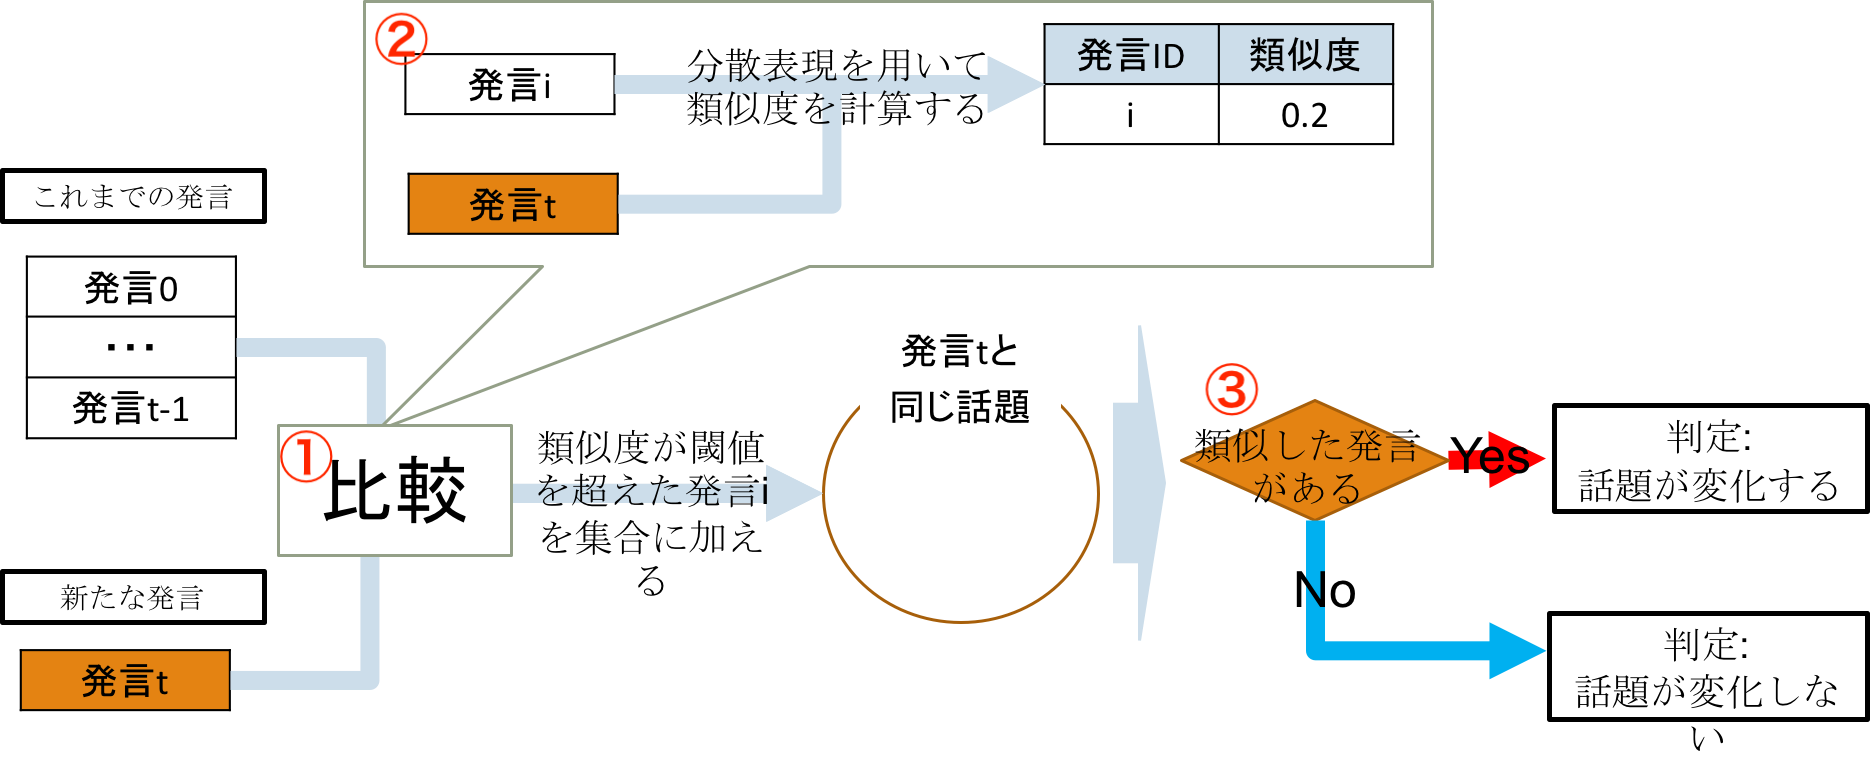
\includegraphics[width=\textwidth]{../images/3.The_Model/WholeModel4.png}
  \caption{システムの流れ}
  \label{Fig:wholeModel}
  \vspace{-10pt}
 \end{center}
\end{figure}

\section{システム詳細}
\label{model:detail}
\subsection{発言データ}
本システムで扱う"発言データ"は単なる文字列ではなく,タイムスタンプ等の他のデータを持つリスト形式のデータである.表\ref{table:remarkData}にデータの一部を示す.
また,以下に本研究で使用する発言データの要素について説明する.
\subsubsection*{\circled{1} id}
発言データを識別するための番号であり,全て整数値で表される.
\subsubsection*{\circled{2} title}
スレッドのタイトル名を表す文字列で,発言がスレッドの先頭でない限りはNULLとなる.
\subsubsection*{\circled{3} body}
発言の内容を表す文字列である.
\subsubsection*{\circled{4} parent-id}
発言の返信先,すなわち親発言のidを表す番号で,親発言がある場合は親発言のidと同じ番号になり,ない場合はNULLとなる.
\subsubsection*{\circled{5} created-at}
発言が投稿された時間を示すタイムスタンプである.

\begin{table}[htbp]
  \begin{tabular}{| c | p{4cm} | p{4cm} | c | p{2cm} | c |} \hline
     %id & title & body & parent-id & user-id & facilitation & created-at & theme-id& has-reply \\ \hline \hline
     id & title & body & parent-id & created-at & $(以降は省略する)$ \\ \hline
     %(ID)&(スレッドタイトル)&(発言内容)&(返信先ID)&(発言者ID)&(ファシリテーター)&(投稿時間)&(議論ID)&(返信)\\ \hline
     18 & オンラインでの議論に関する実験 &  参加者の皆様が集まるまでお待ち下さい。 & NULL & 2017/03/14 16:28:00 & $(以降は省略する)$ \\
     \hline
  \end{tabular}
  \caption{発言データ} \label{table:remarkData}
\end{table}

\subsection{発言間の類似度計算}
\label{model:simRemarkl}
発言間の類似度計算は次の3段階で行われる.
\subsubsection*{\circled{1} 前処理}
本研究では前処理として,発言データ中のtitleとbody,すなわち発言の内容文を対象に\circled{2}で行われる発言内容の類似度計算の精度を上昇させるためにストップワード(役立たないことから処理対象外とされる単語)の除去や単語の重み付けを行う.また,titleがNULLでない場合はtitleとbodyを改行コードで繋いで1つの文章とする.
前処理の詳細については\ref{impl:chapter}章で述べる.
\subsubsection*{\circled{2} 発言内容の類似度計算}
\label{model:simRemark:2}
\circled{1}で行われた前処理の情報や分散表現を用いて発言内容文の類似度計算を行う.
文章間の類似度計算の手法については\ref{impl:chapter}章で詳しく述べる.
\subsubsection*{\circled{3} 総合類似度計算}
上記の\circled{2}で計算された発言の文章間の類似度に発言間の時間差と返信関係を組み合わせることで総合類似度を求める.
\paragraph{時間差評価値}\ \\
新たに投稿された発言$new$とnew以前の発言の1つである$old$間の時間差を式\ref{eq:timeValue}に基いて正規化された評価値として求める.
\begin{equation}
\begin{aligned}
\label{eq:timeValue}
tValue & = 1 - \frac{ epoch(new.created) - epoch(old.created) }{ maxTime }
\end{aligned}
\end{equation}
ここで関数$epoch$及び定数$maxTime$,$x.created$について説明する.$epoch$は与えられたタイムスタンプをエポック秒に変換する.$maxTime$は最大時間差を表し,基本的には議論の制限時間を用いる.$x.created$は発言$x$が投稿された時間を表す.
時間差評価値は0から1の範囲で示され,2発言間の時間差が小さいほど関連が強いとみなし,1 に近くなる.

\paragraph{返信距離}\ \\
返信距離は発言$new$と以前の発言$old$間の返信距離をAlgorithm\ref{algo:replyDist}に基いて再帰的に求められる.

\begin{algorithm}
\caption{返信距離} \label{algo:replyDist}
\begin{algorithmic}[1]
\State $Input:  発言new,発言old,返信距離dist$ \Comment{初期値$dist$=1}
\State $Output: 返信距離dist$
\State $PG = IDに対応づけられた過去の発言の集合;$%~~ Group ~ of ~ past ~ remark
\Procedure{replyDist}{$new,old,dist$} 
	\If{$new$.parent-id == NULL}\label{replyDist:if1-b}
		\State \textbf{return} 0\label{replyDist:if1-e}
	\ElsIf{$new$.parent-id==$old$.id}\label{replyDist:if2-b}
		\State \textbf{return} $dist$\label{replyDist:if2-e}
	 \Else\label{replyDist:if3-b}
	 	\State $parent$ = PG[$new$.parent-id]
		\State $dist+=1$
		\State \textbf{return} REPLYDIST($parent,old,dist$)\label{replyDist:if3-e}
	\EndIf
\EndProcedure
\end{algorithmic}
\end{algorithm}

\ref{replyDist:if1-b} $\sim$ \ref{replyDist:if1-e} 行目で示すように2発言間が返信関係になかった場合は0を返す.
2発言間が返信関係にある場合は\ref{replyDist:if2-b} $\sim$ \ref{replyDist:if2-e}行目 , \ref{replyDist:if3-b} $\sim$ \ref{replyDist:if3-e}行目で示すように発言のidが一致した場合は現在の返信距離を返し,一致しなかった場合は返信距離を1増やして$new$の親発言$parent$と$old$の返信関係を再帰呼び出しで求め,返り値を返す.

\paragraph{総合類似度}\ \\
総合類似度は前述の発言内容の類似度,時間差評価値,返信距離によって求められる.
返信距離が0である時,すなわち2発言が異なるスレッドに属している場合は類似度と時間差評価値から総合類似度を計算する.
総合類似度に時間差評価値を導入した理由は,基本的に少し前に発言に関連して議論が進行されることが多いため,時間的に近いものほど評価を上昇させる仕組みを考慮したからである.
%類似度だけでなく時間差評価値を使用するのは,総合類似度だけで判断してしまうと議論の終盤になって発言数が多くなってきた時に新しく投稿された発言が多くの古い発言と類似していると判断されてしまうことがあり得るからである.理由として,議論は基本的に少し前の発言に関連して行われることが多いことが挙げられる.
時間差評価値を使用して時間的に近しいものほど総合類似度が上昇するようにする.具体的には式\ref{eq:tSimilarity}のように計算される.
\begin{equation}
\begin{aligned}
\label{eq:tSimilarity}
totalSim & = tValue*tWeight + sim*(1-tWeight)
\end{aligned}
\end{equation}

式\ref{eq:tSimilarity}の変数$sim$,$tValue$定数$tWeight$について説明する.$sim$は発言内容の類似度を表し,0から1の値を取る.$tValue$は式\ref{eq:timeValue}での$tValue$と同じもので時間差評価値を表す.$tWeight$は時間差評価値の総合類似度の計算における重要性を表し,0から1の値を取る.
また,返信距離が0でない,すなわち2発言が同じスレッドに属している場合は何らかの関連があると考えられることから,式\ref{eq:tSimilarity2}に示すように時間差評価値を無視して発言内容の類似度に補正値$\alpha$を加えたものを総合類似度として用いる.
\begin{equation}
\begin{aligned}
\label{eq:tSimilarity2}
totalSim & =  sim + \alpha
\end{aligned}
\end{equation}

\section{結言}
\label{model:conclusion}
本章では話題変化判定システムの動作の流れやアルゴリズムについて説明し,扱うデータの形式や内容を示した.
\ref{impl:chapter}章にて説明する発言内容の類似度の計算手法の詳細を除いて,発言間の類似度計算の手法について説明した.
%また,時間的に近しい議論ほど類似度が上昇するように時間差評価値と発言内容の類似度の2つを用いて総合類似度計算することを示した.
また,総合類似度は、時間的に近しい議論ほど類似度が上昇するように時間差評価値と発言内容の類似度から求めることを示した.

 %-------------------------------------------------------------------------------
 \expandafter\ifx\csname MasterFile\endcsname\relax
	\def\BibFile{hoge}
	\expandafter\ifx\csname MasterFile\endcsname\relax
\def\SubFile{hoge}
\documentclass[a4j,12pt,twoside,openany]{jreport}
%\nofiles %tocファイルを更新させない
%\documentclass[12pt,a4j,twoside,openany]{jsbook}
\usepackage[dvipdfmx]{graphicx}
\usepackage{../dspc} % ベースラインスキップの指定
\usepackage{../slashbox} % 表に斜線を入れる
%\usepackage{../mediabb}
\usepackage{fancyvrb} % Verbatim環境
\usepackage{fancyhdr} % Headerの下線付き章見出し
\usepackage{here} % float[H]
\usepackage{multirow}
\usepackage{hhline} % 表の罫線の角を美しくする
\usepackage{amsmath} %コレがないとcasesが動かない
\usepackage{amsfonts} % 数学用フォント
\usepackage{bm} % 数式環境での bold
\usepackage{algorithm}
\usepackage{algorithmicx}
\usepackage[noend]{algpseudocode}%\procedureはここに含まれる
\usepackage[flushleft]{threeparttable} % 脚注付きテーブル
\usepackage{enumitem}
\usepackage{comment}
\usepackage{fancybox}
%\usepackage{csvsimple,booktabs,siunitx}
%\usepackage{filecontents}
\usepackage{ulinej}


\setlength{\evensidemargin}{5pt}
\setlength{\oddsidemargin}{40pt}
%\setlength{\headheight}{16.5pt}
%%\setlength{\headheight}{30pt}
\setcounter{secnumdepth}{3}
\setlist[description]{leftmargin=2\parindent,labelindent=\parindent}

\makeatletter
\def\@makechapterhead#1{%
	\vspace*{50\p@}%
	{
		\parindent \z@ \raggedright \normalfont
		\ifnum \c@secnumdepth >\m@ne
		% \if@mainmatter
			\huge\bfseries\@chapapp\thechapter\@chappos
			\par\nobreak
			\vskip 20\p@
		% \fi
		\fi
		\interlinepenalty\@M
		\Huge\bfseries #1\par\nobreak
		\vskip 40\p@
	}
}

%新しいコマンド定義
\newcounter{linenumber}
\newenvironment{listing}{%
  \begin{list}{%
    \small\arabic{linenumber}:}{%
      \usecounter{linenumber}%
      \setlength{\baselineskip}{18pt}%
      \setlength{\itemsep}{0pt}%
      \setlength{\parsep}{0pt}}}%
 {\end{list}}
\newcommand{\figcaption}[1]{\def\@captype{figure}\caption{#1}}
\newcommand{\tblcaption}[1]{\def\@captype{table}\caption{#1}}
\newcommand{\norm}[1]{\left\| #1 \right\|}
\newcommand{\cc}[1]{\multicolumn{1}{|c|}{#1}}
\newcommand{\circled}[1]{\raisebox{.5pt}{\textcircled{\raisebox{-.9pt} {#1}}}}
\newcommand{\specialcell}[2][c]{%
  \begin{tabular}[#1]{@{}c@{}}#2\end{tabular}}
\makeatother
%===============================================================================
\expandafter\ifx\csname SubFile\endcsname\relax
\begin{document}
\def\MasterFile{hoge}
%-------------------------------------------------------------------------------
%\maketitle
\thispagestyle{empty}
\documentclass[a4j,12pt]{jarticle}
% 外表紙

% 題名
\def\title{降水量予測のための\\Sequence-to-Sequenceモデルに基づく\\マルチモーダル学習}
% 著者
\def\author{林 政行}
% 入学年度(平成)
\def\year{24}
% 学籍番号
\def\number{24115113}
% 指導教官
\def\kyoukan{伊藤孝行}
% 指導教官役職
\def\kyoukanrank{教授}
% 提出日
\def\teisyutubi{平成28年2月8日}

\begin{document}
\pagestyle{empty}
\baselineskip=18pt

\begin{center}

\vspace*{2cm}

{\huge \textbf{卒業論文}}

\vspace*{3cm}

%\vrule width 10cm height 1pt depth 0pt



%(題目)
%\vspace{5pt}
%\hrule height 3pt
%\vspace{1zh}

\vrule width 6.25cm height 6pt depth -2pt
\makebox[1.5cm]{(題目)}
\vrule width 6.25cm height 6pt depth -2pt

{\LARGE {\title}}

\vspace{1zh}
%{\large {\subtitle}}
%\hrule height 3pt
\vrule width 14cm height 4pt depth 0pt

\vspace*{1cm}

指導教員 {\large {\kyoukan}} {\kyoukanrank}

%\vspace*{5cm}
\vfill

{\large 名古屋工業大学 情報工学科}

{\large 平成{\year}年度 入学 ({\number})}

\vspace*{1cm}

%{\huge\mc {\author}}

\underline{(氏名)\hspace{3zw}{\huge\mc {\author}}\hspace{3zw}}

\vspace*{1cm}

({\teisyutubi}提出)

\vspace{2cm}
\end{center}

\end{document}
\begin{titlepage}

% 題名
\def\title{分散表現を用いた\\話題変化判定}
% 補助題名
\def\subtitle{卒業論文}
% 著者
\def\author{芳野 魁}
% 入学年度(平成)
\def\year{29}
% 学籍番号
\def\number{26115162}
% 指導教官
\def\kyoukan{伊藤 孝行}
% 指導教官役職
\def\kyoukanrank{教授}
% 提出日
\def\teisyutubi{平成29年9月19日}

\pagestyle{empty}

\begin{center}

\vspace*{20mm}
{\Large\mc 平成29年度 \hspace{7mm} 卒 業 論 文}
\vspace{15mm}

%\setlength{\unitlength}{1mm}
\begin{picture}(100,60)
  \put(0,0){\makebox(100,60){\huge\bf\shortstack{\title}}}
\end{picture}
\\
%\begin{picture}(100,5)
%  \put(0,0){\makebox(100,5){\Large\bf\shortstack{\subtitle}}}
%\end{picture}
\end{center}
\vspace{10mm}
\begin{flushright}
\begin{tabular}{ll}
{\large 提出日} & {\large {\teisyutubi}} \\
{\large 所属}  & {\large 名古屋工業大学 情報工学科} \\
{\large 指導教員} & {\large {\kyoukan} {\kyoukanrank}} \\
 & \\
{\large 入学年度} & {\large 平成{\year}年度入学}\\
{\large 学籍番号} &{\large {\number}} \\
 & \\
%{\large 氏名} & {\huge {\author}}
{\large 氏名} & {\huge\mc {\author}}
\end{tabular}
\end{flushright}

\end{titlepage}

%\addcontentsline{toc}{chapter}{表紙}
\thispagestyle{empty}
\mbox{}\newpage
%===============================================================================
%\frontmatter
%===============================================================================
%\mainmatter
%-------------------------------------------------------------------------------
\pagenumbering{arabic}
\cleardoublepage
\expandafter\ifx\csname MasterFile\endcsname\relax
\def\SubFile{hoge}
\input{../thesis/thesis}
\begin{document}
\fi
%-------------------------------------------------------------------------------
\cleardoublepage
\chapter*{論文要旨}\addcontentsline{toc}{chapter}{論文要旨}
近年,Web上での大規模な議論活動が活発になっているが,現在一般的に使われている "2ちゃんねる" や "Twitter" といったシステムでは整理や収束を行うことが困難である.困難である原因として,議論の管理を行う者がいないことが挙げられる.
議論を収束させるには議論のマネジメントを行う人物が必要である.
%
大規模意見集約システムCOLLAGREEではファシリテーターと呼ばれる人物が議論のマネジメントを行っている.
しかし,ファシリテーターは人間であり,長時間に渡って大人数での議論の動向をマネジメントし続けるのは困難である.
%
COLLAGREEで大規模な議論を収束させるためには,ファシリテーターが必要な時にだけ画面を見るようにして画面に向き合う時間を減らす工夫があることが望ましい.ファシリテーターが画面を見るべきタイミングは議論の話題が変化したときである.以前の議論の内容から外れた発言がされた時,ファシリテーターが適切に発言することで,脱線や炎上を避けて議論を収束させることができる.
すなわち,ファシリテーターの代わりに自動的に議論中の話題の変化を事前に判定することが求められている.
%
現在,COLLAGREE上で使用されている議論支援システムは投稿支援システムと議論可視化システムの2つに大別できる.
投稿支援システムはポイント機能やファシリテーションフレーズ簡易投稿機能のように,ユーザーが投稿をする際に何らかの補助やリアクションを行う.現行の機能では選択肢の提示に留まっており,作業量を減らすことには繋がりにくい。
一方,議論可視化システムは議論ツリーやキーワード抽出のように,ユーザーにスレッドとは異なる議論の見方を提供する.現行の機能では議論を見やすくすることに重点が置かれており,議論の把握の助けにはなるが画面に向き合う時間を減らすことにはなりにくい.むしろ,作業量を増やすことになり得る機能もある.
\begin{comment}
ポイント機能(ユーザの議論行動を活性化)-1
ファシリテーションフレーズ簡易投稿機能-1
議論ツリー-2
1文の要約,スレッドの要約,クラスタリング,返信意見の極性判定-2
ファシリテーションスタンプ-1
キーワード抽出-2
いいね機能-1
いいねランキング-2
投票機能-1
議論フェーズ機能-2
1-意見を出す、投稿をする際に補助や選択肢、リアクションを与える
2-議論の別の見方を提供する
\end{comment}
%
近年,自然言語処理の分野において分散表現が多くの研究で使われており,機械翻訳を始めとする単語の意味が重要となる分野で精度の向上が確認されている.分散表現を用いることで,人間に近い精度で話題の変化を観測することが可能となる.
%
以上のような背景を踏まえて,分散表現を用いて,話題の変化を観測し,話題の変化が確認された時にファシリテーターに伝えることが望ましい.
話題の変化の観測は,発言中に現れる単語の関連度合いの計算と見なすことができる.
分散表現を用いることで単語間の類似度を求めることができる,値が大きいほど単語がそれぞれ類似した実数ベクトルであることを表す.単語Aと単語Bの実数ベクトルが類似しているとは,単語Aと共に使われることの多い単語と単語Bと共に使われることの多い単語が多く共通していることを示す.故に,分散表現を使って単語の関連度を計算することができる.
%
発言文から単語を選ぶ際には自動要約を用いる.発言文から重要でない単語を取り除くことで関連度の計算の精度を高めることが可能となる.
%
本論文では,分散表現を用いて議論中での発言に含まれる単語の関連度を計算し,話題の変化を観測する手法を提案する.
%
提案手法は,既存の抽出的要約手法を用いて選ばれた単語の関連度を計算する手法,Seq2Seqによる生成的要約を用いて生成された単語の関連度を計算する手法,オントロジーを用いて求められた単語の関連度を計算する手法の3つである.
提案した3つの手法により,議論中の話題の変化の観測の評価実験を行い,各手法の評価を行う.
評価実験によって,提案手法を用いることで人間の代わりに自動的に話題の変化を観測できることを確認する.
%
 \begin{comment}
大規模な議論では意見を共有することは可能であるが,議論を整理させることや収束させることは難しい.以上から大規模意見集約システムCOLLAGREEが開発された.本システムではWeb上で適切に大規模な議論を行うことができるように議論をマネジメントするファシリテーターを導入した.
過去の実験ではファシリテーターの存在が議論の集約に大きな役割を果たしていることが認識されており,大規模な議論のためにファシリテータは必要である.しかし,議論の規模に伴って議論時間が長くなる傾向があり,同時にファシリテーターは常に議論の動向を見続ける必要がある.故に,議論の規模が大きくなればなるほどファシリテーターは長時間かつ大規模な議論の動向の監視によって大きな負担がかかる.大規模な議論が増加する傾向を踏まえるとファシリテーターにかかる負担を軽減する支援が必要となることは明白である.
また,近年自然言語処理の分野において分散表現が多くの研究で使われており,機械翻訳を始めとする複数の分野で精度の向上が確認されている.まだ適応されていない分野でも結果の向上が期待できる.
従って,本研究では負担軽減の1つとして分散表現を用いて議論中での話題の変化を人間の代わりに検知することでファシリテーターの負担を軽減することを目指す.
-----------------

\end{comment}
%-------------------------------------------------------------------------------
\expandafter\ifx\csname MasterFile\endcsname\relax
\end{document}
\fi

%-------------------------------------------------------------------------------
\clearpage
\addcontentsline{toc}{chapter}{目次}
\tableofcontents

\clearpage
\addcontentsline{toc}{chapter}{図目次}
\listoffigures

\clearpage
\addcontentsline{toc}{chapter}{表目次}
\listoftables

%-------------------------------------------------------------------------------

%=====================
\pagestyle{fancy} % Headerをつける
\renewcommand{\sectionmark}[1]{\markright{\thesection\ \ \ #1}}
\renewcommand{\chaptermark}[1]{\markboth{#1}{}}
\lhead{}
\chead{}
\lfoot{}
\rfoot{}%-------------------------------------------------------------------------------
\expandafter\ifx\csname MasterFile\endcsname\relax
\def\SubFile{hoge}
\input{../thesis/thesis}
\begin{document}
\fi
%-------------------------------------------------------------------------------
\cleardoublepage
\chapter*{論文要旨}\addcontentsline{toc}{chapter}{論文要旨}
近年,Web上での大規模な議論活動が活発になっているが,現在一般的に使われている "2ちゃんねる" や "Twitter" といったシステムでは整理や収束を行うことが困難である.困難である原因として,議論の管理を行う者がいないことが挙げられる.
議論を収束させるには議論のマネジメントを行う人物が必要である.
%
大規模意見集約システムCOLLAGREEではファシリテーターと呼ばれる人物が議論のマネジメントを行っている.
しかし,ファシリテーターは人間であり,長時間に渡って大人数での議論の動向をマネジメントし続けるのは困難である.
%
COLLAGREEで大規模な議論を収束させるためには,ファシリテーターが必要な時にだけ画面を見るようにして画面に向き合う時間を減らす工夫があることが望ましい.ファシリテーターが画面を見るべきタイミングは議論の話題が変化したときである.以前の議論の内容から外れた発言がされた時,ファシリテーターが適切に発言することで,脱線や炎上を避けて議論を収束させることができる.
すなわち,ファシリテーターの代わりに自動的に議論中の話題の変化を事前に判定することが求められている.
%
現在,COLLAGREE上で使用されている議論支援システムは投稿支援システムと議論可視化システムの2つに大別できる.
投稿支援システムはポイント機能やファシリテーションフレーズ簡易投稿機能のように,ユーザーが投稿をする際に何らかの補助やリアクションを行う.現行の機能では選択肢の提示に留まっており,作業量を減らすことには繋がりにくい。
一方,議論可視化システムは議論ツリーやキーワード抽出のように,ユーザーにスレッドとは異なる議論の見方を提供する.現行の機能では議論を見やすくすることに重点が置かれており,議論の把握の助けにはなるが画面に向き合う時間を減らすことにはなりにくい.むしろ,作業量を増やすことになり得る機能もある.
\begin{comment}
ポイント機能(ユーザの議論行動を活性化)-1
ファシリテーションフレーズ簡易投稿機能-1
議論ツリー-2
1文の要約,スレッドの要約,クラスタリング,返信意見の極性判定-2
ファシリテーションスタンプ-1
キーワード抽出-2
いいね機能-1
いいねランキング-2
投票機能-1
議論フェーズ機能-2
1-意見を出す、投稿をする際に補助や選択肢、リアクションを与える
2-議論の別の見方を提供する
\end{comment}
%
近年,自然言語処理の分野において分散表現が多くの研究で使われており,機械翻訳を始めとする単語の意味が重要となる分野で精度の向上が確認されている.分散表現を用いることで,人間に近い精度で話題の変化を観測することが可能となる.
%
以上のような背景を踏まえて,分散表現を用いて,話題の変化を観測し,話題の変化が確認された時にファシリテーターに伝えることが望ましい.
話題の変化の観測は,発言中に現れる単語の関連度合いの計算と見なすことができる.
分散表現を用いることで単語間の類似度を求めることができる,値が大きいほど単語がそれぞれ類似した実数ベクトルであることを表す.単語Aと単語Bの実数ベクトルが類似しているとは,単語Aと共に使われることの多い単語と単語Bと共に使われることの多い単語が多く共通していることを示す.故に,分散表現を使って単語の関連度を計算することができる.
%
発言文から単語を選ぶ際には自動要約を用いる.発言文から重要でない単語を取り除くことで関連度の計算の精度を高めることが可能となる.
%
本論文では,分散表現を用いて議論中での発言に含まれる単語の関連度を計算し,話題の変化を観測する手法を提案する.
%
提案手法は,既存の抽出的要約手法を用いて選ばれた単語の関連度を計算する手法,Seq2Seqによる生成的要約を用いて生成された単語の関連度を計算する手法,オントロジーを用いて求められた単語の関連度を計算する手法の3つである.
提案した3つの手法により,議論中の話題の変化の観測の評価実験を行い,各手法の評価を行う.
評価実験によって,提案手法を用いることで人間の代わりに自動的に話題の変化を観測できることを確認する.
%
 \begin{comment}
大規模な議論では意見を共有することは可能であるが,議論を整理させることや収束させることは難しい.以上から大規模意見集約システムCOLLAGREEが開発された.本システムではWeb上で適切に大規模な議論を行うことができるように議論をマネジメントするファシリテーターを導入した.
過去の実験ではファシリテーターの存在が議論の集約に大きな役割を果たしていることが認識されており,大規模な議論のためにファシリテータは必要である.しかし,議論の規模に伴って議論時間が長くなる傾向があり,同時にファシリテーターは常に議論の動向を見続ける必要がある.故に,議論の規模が大きくなればなるほどファシリテーターは長時間かつ大規模な議論の動向の監視によって大きな負担がかかる.大規模な議論が増加する傾向を踏まえるとファシリテーターにかかる負担を軽減する支援が必要となることは明白である.
また,近年自然言語処理の分野において分散表現が多くの研究で使われており,機械翻訳を始めとする複数の分野で精度の向上が確認されている.まだ適応されていない分野でも結果の向上が期待できる.
従って,本研究では負担軽減の1つとして分散表現を用いて議論中での話題の変化を人間の代わりに検知することでファシリテーターの負担を軽減することを目指す.
-----------------

\end{comment}
%-------------------------------------------------------------------------------
\expandafter\ifx\csname MasterFile\endcsname\relax
\end{document}
\fi

%-------------------------------------------------------------------------------
\expandafter\ifx\csname MasterFile\endcsname\relax
\def\SubFile{hoge}
\input{../thesis/thesis}
\begin{document}
\fi
%-------------------------------------------------------------------------------
\cleardoublepage
\chapter*{論文要旨}\addcontentsline{toc}{chapter}{論文要旨}
近年,Web上での大規模な議論活動が活発になっているが,現在一般的に使われている "2ちゃんねる" や "Twitter" といったシステムでは整理や収束を行うことが困難である.困難である原因として,議論の管理を行う者がいないことが挙げられる.
議論を収束させるには議論のマネジメントを行う人物が必要である.
%
大規模意見集約システムCOLLAGREEではファシリテーターと呼ばれる人物が議論のマネジメントを行っている.
しかし,ファシリテーターは人間であり,長時間に渡って大人数での議論の動向をマネジメントし続けるのは困難である.
%
COLLAGREEで大規模な議論を収束させるためには,ファシリテーターが必要な時にだけ画面を見るようにして画面に向き合う時間を減らす工夫があることが望ましい.ファシリテーターが画面を見るべきタイミングは議論の話題が変化したときである.以前の議論の内容から外れた発言がされた時,ファシリテーターが適切に発言することで,脱線や炎上を避けて議論を収束させることができる.
すなわち,ファシリテーターの代わりに自動的に議論中の話題の変化を事前に判定することが求められている.
%
現在,COLLAGREE上で使用されている議論支援システムは投稿支援システムと議論可視化システムの2つに大別できる.
投稿支援システムはポイント機能やファシリテーションフレーズ簡易投稿機能のように,ユーザーが投稿をする際に何らかの補助やリアクションを行う.現行の機能では選択肢の提示に留まっており,作業量を減らすことには繋がりにくい。
一方,議論可視化システムは議論ツリーやキーワード抽出のように,ユーザーにスレッドとは異なる議論の見方を提供する.現行の機能では議論を見やすくすることに重点が置かれており,議論の把握の助けにはなるが画面に向き合う時間を減らすことにはなりにくい.むしろ,作業量を増やすことになり得る機能もある.
\begin{comment}
ポイント機能(ユーザの議論行動を活性化)-1
ファシリテーションフレーズ簡易投稿機能-1
議論ツリー-2
1文の要約,スレッドの要約,クラスタリング,返信意見の極性判定-2
ファシリテーションスタンプ-1
キーワード抽出-2
いいね機能-1
いいねランキング-2
投票機能-1
議論フェーズ機能-2
1-意見を出す、投稿をする際に補助や選択肢、リアクションを与える
2-議論の別の見方を提供する
\end{comment}
%
近年,自然言語処理の分野において分散表現が多くの研究で使われており,機械翻訳を始めとする単語の意味が重要となる分野で精度の向上が確認されている.分散表現を用いることで,人間に近い精度で話題の変化を観測することが可能となる.
%
以上のような背景を踏まえて,分散表現を用いて,話題の変化を観測し,話題の変化が確認された時にファシリテーターに伝えることが望ましい.
話題の変化の観測は,発言中に現れる単語の関連度合いの計算と見なすことができる.
分散表現を用いることで単語間の類似度を求めることができる,値が大きいほど単語がそれぞれ類似した実数ベクトルであることを表す.単語Aと単語Bの実数ベクトルが類似しているとは,単語Aと共に使われることの多い単語と単語Bと共に使われることの多い単語が多く共通していることを示す.故に,分散表現を使って単語の関連度を計算することができる.
%
発言文から単語を選ぶ際には自動要約を用いる.発言文から重要でない単語を取り除くことで関連度の計算の精度を高めることが可能となる.
%
本論文では,分散表現を用いて議論中での発言に含まれる単語の関連度を計算し,話題の変化を観測する手法を提案する.
%
提案手法は,既存の抽出的要約手法を用いて選ばれた単語の関連度を計算する手法,Seq2Seqによる生成的要約を用いて生成された単語の関連度を計算する手法,オントロジーを用いて求められた単語の関連度を計算する手法の3つである.
提案した3つの手法により,議論中の話題の変化の観測の評価実験を行い,各手法の評価を行う.
評価実験によって,提案手法を用いることで人間の代わりに自動的に話題の変化を観測できることを確認する.
%
 \begin{comment}
大規模な議論では意見を共有することは可能であるが,議論を整理させることや収束させることは難しい.以上から大規模意見集約システムCOLLAGREEが開発された.本システムではWeb上で適切に大規模な議論を行うことができるように議論をマネジメントするファシリテーターを導入した.
過去の実験ではファシリテーターの存在が議論の集約に大きな役割を果たしていることが認識されており,大規模な議論のためにファシリテータは必要である.しかし,議論の規模に伴って議論時間が長くなる傾向があり,同時にファシリテーターは常に議論の動向を見続ける必要がある.故に,議論の規模が大きくなればなるほどファシリテーターは長時間かつ大規模な議論の動向の監視によって大きな負担がかかる.大規模な議論が増加する傾向を踏まえるとファシリテーターにかかる負担を軽減する支援が必要となることは明白である.
また,近年自然言語処理の分野において分散表現が多くの研究で使われており,機械翻訳を始めとする複数の分野で精度の向上が確認されている.まだ適応されていない分野でも結果の向上が期待できる.
従って,本研究では負担軽減の1つとして分散表現を用いて議論中での話題の変化を人間の代わりに検知することでファシリテーターの負担を軽減することを目指す.
-----------------

\end{comment}
%-------------------------------------------------------------------------------
\expandafter\ifx\csname MasterFile\endcsname\relax
\end{document}
\fi

%-------------------------------------------------------------------------------
\expandafter\ifx\csname MasterFile\endcsname\relax
\def\SubFile{hoge}
\input{../thesis/thesis}
\begin{document}
\fi
%-------------------------------------------------------------------------------
\cleardoublepage
\chapter*{論文要旨}\addcontentsline{toc}{chapter}{論文要旨}
近年,Web上での大規模な議論活動が活発になっているが,現在一般的に使われている "2ちゃんねる" や "Twitter" といったシステムでは整理や収束を行うことが困難である.困難である原因として,議論の管理を行う者がいないことが挙げられる.
議論を収束させるには議論のマネジメントを行う人物が必要である.
%
大規模意見集約システムCOLLAGREEではファシリテーターと呼ばれる人物が議論のマネジメントを行っている.
しかし,ファシリテーターは人間であり,長時間に渡って大人数での議論の動向をマネジメントし続けるのは困難である.
%
COLLAGREEで大規模な議論を収束させるためには,ファシリテーターが必要な時にだけ画面を見るようにして画面に向き合う時間を減らす工夫があることが望ましい.ファシリテーターが画面を見るべきタイミングは議論の話題が変化したときである.以前の議論の内容から外れた発言がされた時,ファシリテーターが適切に発言することで,脱線や炎上を避けて議論を収束させることができる.
すなわち,ファシリテーターの代わりに自動的に議論中の話題の変化を事前に判定することが求められている.
%
現在,COLLAGREE上で使用されている議論支援システムは投稿支援システムと議論可視化システムの2つに大別できる.
投稿支援システムはポイント機能やファシリテーションフレーズ簡易投稿機能のように,ユーザーが投稿をする際に何らかの補助やリアクションを行う.現行の機能では選択肢の提示に留まっており,作業量を減らすことには繋がりにくい。
一方,議論可視化システムは議論ツリーやキーワード抽出のように,ユーザーにスレッドとは異なる議論の見方を提供する.現行の機能では議論を見やすくすることに重点が置かれており,議論の把握の助けにはなるが画面に向き合う時間を減らすことにはなりにくい.むしろ,作業量を増やすことになり得る機能もある.
\begin{comment}
ポイント機能(ユーザの議論行動を活性化)-1
ファシリテーションフレーズ簡易投稿機能-1
議論ツリー-2
1文の要約,スレッドの要約,クラスタリング,返信意見の極性判定-2
ファシリテーションスタンプ-1
キーワード抽出-2
いいね機能-1
いいねランキング-2
投票機能-1
議論フェーズ機能-2
1-意見を出す、投稿をする際に補助や選択肢、リアクションを与える
2-議論の別の見方を提供する
\end{comment}
%
近年,自然言語処理の分野において分散表現が多くの研究で使われており,機械翻訳を始めとする単語の意味が重要となる分野で精度の向上が確認されている.分散表現を用いることで,人間に近い精度で話題の変化を観測することが可能となる.
%
以上のような背景を踏まえて,分散表現を用いて,話題の変化を観測し,話題の変化が確認された時にファシリテーターに伝えることが望ましい.
話題の変化の観測は,発言中に現れる単語の関連度合いの計算と見なすことができる.
分散表現を用いることで単語間の類似度を求めることができる,値が大きいほど単語がそれぞれ類似した実数ベクトルであることを表す.単語Aと単語Bの実数ベクトルが類似しているとは,単語Aと共に使われることの多い単語と単語Bと共に使われることの多い単語が多く共通していることを示す.故に,分散表現を使って単語の関連度を計算することができる.
%
発言文から単語を選ぶ際には自動要約を用いる.発言文から重要でない単語を取り除くことで関連度の計算の精度を高めることが可能となる.
%
本論文では,分散表現を用いて議論中での発言に含まれる単語の関連度を計算し,話題の変化を観測する手法を提案する.
%
提案手法は,既存の抽出的要約手法を用いて選ばれた単語の関連度を計算する手法,Seq2Seqによる生成的要約を用いて生成された単語の関連度を計算する手法,オントロジーを用いて求められた単語の関連度を計算する手法の3つである.
提案した3つの手法により,議論中の話題の変化の観測の評価実験を行い,各手法の評価を行う.
評価実験によって,提案手法を用いることで人間の代わりに自動的に話題の変化を観測できることを確認する.
%
 \begin{comment}
大規模な議論では意見を共有することは可能であるが,議論を整理させることや収束させることは難しい.以上から大規模意見集約システムCOLLAGREEが開発された.本システムではWeb上で適切に大規模な議論を行うことができるように議論をマネジメントするファシリテーターを導入した.
過去の実験ではファシリテーターの存在が議論の集約に大きな役割を果たしていることが認識されており,大規模な議論のためにファシリテータは必要である.しかし,議論の規模に伴って議論時間が長くなる傾向があり,同時にファシリテーターは常に議論の動向を見続ける必要がある.故に,議論の規模が大きくなればなるほどファシリテーターは長時間かつ大規模な議論の動向の監視によって大きな負担がかかる.大規模な議論が増加する傾向を踏まえるとファシリテーターにかかる負担を軽減する支援が必要となることは明白である.
また,近年自然言語処理の分野において分散表現が多くの研究で使われており,機械翻訳を始めとする複数の分野で精度の向上が確認されている.まだ適応されていない分野でも結果の向上が期待できる.
従って,本研究では負担軽減の1つとして分散表現を用いて議論中での話題の変化を人間の代わりに検知することでファシリテーターの負担を軽減することを目指す.
-----------------

\end{comment}
%-------------------------------------------------------------------------------
\expandafter\ifx\csname MasterFile\endcsname\relax
\end{document}
\fi

%-------------------------------------------------------------------------------
\expandafter\ifx\csname MasterFile\endcsname\relax
\def\SubFile{hoge}
\input{../thesis/thesis}
\begin{document}
\fi
%-------------------------------------------------------------------------------
\cleardoublepage
\chapter*{論文要旨}\addcontentsline{toc}{chapter}{論文要旨}
近年,Web上での大規模な議論活動が活発になっているが,現在一般的に使われている "2ちゃんねる" や "Twitter" といったシステムでは整理や収束を行うことが困難である.困難である原因として,議論の管理を行う者がいないことが挙げられる.
議論を収束させるには議論のマネジメントを行う人物が必要である.
%
大規模意見集約システムCOLLAGREEではファシリテーターと呼ばれる人物が議論のマネジメントを行っている.
しかし,ファシリテーターは人間であり,長時間に渡って大人数での議論の動向をマネジメントし続けるのは困難である.
%
COLLAGREEで大規模な議論を収束させるためには,ファシリテーターが必要な時にだけ画面を見るようにして画面に向き合う時間を減らす工夫があることが望ましい.ファシリテーターが画面を見るべきタイミングは議論の話題が変化したときである.以前の議論の内容から外れた発言がされた時,ファシリテーターが適切に発言することで,脱線や炎上を避けて議論を収束させることができる.
すなわち,ファシリテーターの代わりに自動的に議論中の話題の変化を事前に判定することが求められている.
%
現在,COLLAGREE上で使用されている議論支援システムは投稿支援システムと議論可視化システムの2つに大別できる.
投稿支援システムはポイント機能やファシリテーションフレーズ簡易投稿機能のように,ユーザーが投稿をする際に何らかの補助やリアクションを行う.現行の機能では選択肢の提示に留まっており,作業量を減らすことには繋がりにくい。
一方,議論可視化システムは議論ツリーやキーワード抽出のように,ユーザーにスレッドとは異なる議論の見方を提供する.現行の機能では議論を見やすくすることに重点が置かれており,議論の把握の助けにはなるが画面に向き合う時間を減らすことにはなりにくい.むしろ,作業量を増やすことになり得る機能もある.
\begin{comment}
ポイント機能(ユーザの議論行動を活性化)-1
ファシリテーションフレーズ簡易投稿機能-1
議論ツリー-2
1文の要約,スレッドの要約,クラスタリング,返信意見の極性判定-2
ファシリテーションスタンプ-1
キーワード抽出-2
いいね機能-1
いいねランキング-2
投票機能-1
議論フェーズ機能-2
1-意見を出す、投稿をする際に補助や選択肢、リアクションを与える
2-議論の別の見方を提供する
\end{comment}
%
近年,自然言語処理の分野において分散表現が多くの研究で使われており,機械翻訳を始めとする単語の意味が重要となる分野で精度の向上が確認されている.分散表現を用いることで,人間に近い精度で話題の変化を観測することが可能となる.
%
以上のような背景を踏まえて,分散表現を用いて,話題の変化を観測し,話題の変化が確認された時にファシリテーターに伝えることが望ましい.
話題の変化の観測は,発言中に現れる単語の関連度合いの計算と見なすことができる.
分散表現を用いることで単語間の類似度を求めることができる,値が大きいほど単語がそれぞれ類似した実数ベクトルであることを表す.単語Aと単語Bの実数ベクトルが類似しているとは,単語Aと共に使われることの多い単語と単語Bと共に使われることの多い単語が多く共通していることを示す.故に,分散表現を使って単語の関連度を計算することができる.
%
発言文から単語を選ぶ際には自動要約を用いる.発言文から重要でない単語を取り除くことで関連度の計算の精度を高めることが可能となる.
%
本論文では,分散表現を用いて議論中での発言に含まれる単語の関連度を計算し,話題の変化を観測する手法を提案する.
%
提案手法は,既存の抽出的要約手法を用いて選ばれた単語の関連度を計算する手法,Seq2Seqによる生成的要約を用いて生成された単語の関連度を計算する手法,オントロジーを用いて求められた単語の関連度を計算する手法の3つである.
提案した3つの手法により,議論中の話題の変化の観測の評価実験を行い,各手法の評価を行う.
評価実験によって,提案手法を用いることで人間の代わりに自動的に話題の変化を観測できることを確認する.
%
 \begin{comment}
大規模な議論では意見を共有することは可能であるが,議論を整理させることや収束させることは難しい.以上から大規模意見集約システムCOLLAGREEが開発された.本システムではWeb上で適切に大規模な議論を行うことができるように議論をマネジメントするファシリテーターを導入した.
過去の実験ではファシリテーターの存在が議論の集約に大きな役割を果たしていることが認識されており,大規模な議論のためにファシリテータは必要である.しかし,議論の規模に伴って議論時間が長くなる傾向があり,同時にファシリテーターは常に議論の動向を見続ける必要がある.故に,議論の規模が大きくなればなるほどファシリテーターは長時間かつ大規模な議論の動向の監視によって大きな負担がかかる.大規模な議論が増加する傾向を踏まえるとファシリテーターにかかる負担を軽減する支援が必要となることは明白である.
また,近年自然言語処理の分野において分散表現が多くの研究で使われており,機械翻訳を始めとする複数の分野で精度の向上が確認されている.まだ適応されていない分野でも結果の向上が期待できる.
従って,本研究では負担軽減の1つとして分散表現を用いて議論中での話題の変化を人間の代わりに検知することでファシリテーターの負担を軽減することを目指す.
-----------------

\end{comment}
%-------------------------------------------------------------------------------
\expandafter\ifx\csname MasterFile\endcsname\relax
\end{document}
\fi

%-------------------------------------------------------------------------------
\expandafter\ifx\csname MasterFile\endcsname\relax
\def\SubFile{hoge}
\input{../thesis/thesis}
\begin{document}
\fi
%-------------------------------------------------------------------------------
\cleardoublepage
\chapter*{論文要旨}\addcontentsline{toc}{chapter}{論文要旨}
近年,Web上での大規模な議論活動が活発になっているが,現在一般的に使われている "2ちゃんねる" や "Twitter" といったシステムでは整理や収束を行うことが困難である.困難である原因として,議論の管理を行う者がいないことが挙げられる.
議論を収束させるには議論のマネジメントを行う人物が必要である.
%
大規模意見集約システムCOLLAGREEではファシリテーターと呼ばれる人物が議論のマネジメントを行っている.
しかし,ファシリテーターは人間であり,長時間に渡って大人数での議論の動向をマネジメントし続けるのは困難である.
%
COLLAGREEで大規模な議論を収束させるためには,ファシリテーターが必要な時にだけ画面を見るようにして画面に向き合う時間を減らす工夫があることが望ましい.ファシリテーターが画面を見るべきタイミングは議論の話題が変化したときである.以前の議論の内容から外れた発言がされた時,ファシリテーターが適切に発言することで,脱線や炎上を避けて議論を収束させることができる.
すなわち,ファシリテーターの代わりに自動的に議論中の話題の変化を事前に判定することが求められている.
%
現在,COLLAGREE上で使用されている議論支援システムは投稿支援システムと議論可視化システムの2つに大別できる.
投稿支援システムはポイント機能やファシリテーションフレーズ簡易投稿機能のように,ユーザーが投稿をする際に何らかの補助やリアクションを行う.現行の機能では選択肢の提示に留まっており,作業量を減らすことには繋がりにくい。
一方,議論可視化システムは議論ツリーやキーワード抽出のように,ユーザーにスレッドとは異なる議論の見方を提供する.現行の機能では議論を見やすくすることに重点が置かれており,議論の把握の助けにはなるが画面に向き合う時間を減らすことにはなりにくい.むしろ,作業量を増やすことになり得る機能もある.
\begin{comment}
ポイント機能(ユーザの議論行動を活性化)-1
ファシリテーションフレーズ簡易投稿機能-1
議論ツリー-2
1文の要約,スレッドの要約,クラスタリング,返信意見の極性判定-2
ファシリテーションスタンプ-1
キーワード抽出-2
いいね機能-1
いいねランキング-2
投票機能-1
議論フェーズ機能-2
1-意見を出す、投稿をする際に補助や選択肢、リアクションを与える
2-議論の別の見方を提供する
\end{comment}
%
近年,自然言語処理の分野において分散表現が多くの研究で使われており,機械翻訳を始めとする単語の意味が重要となる分野で精度の向上が確認されている.分散表現を用いることで,人間に近い精度で話題の変化を観測することが可能となる.
%
以上のような背景を踏まえて,分散表現を用いて,話題の変化を観測し,話題の変化が確認された時にファシリテーターに伝えることが望ましい.
話題の変化の観測は,発言中に現れる単語の関連度合いの計算と見なすことができる.
分散表現を用いることで単語間の類似度を求めることができる,値が大きいほど単語がそれぞれ類似した実数ベクトルであることを表す.単語Aと単語Bの実数ベクトルが類似しているとは,単語Aと共に使われることの多い単語と単語Bと共に使われることの多い単語が多く共通していることを示す.故に,分散表現を使って単語の関連度を計算することができる.
%
発言文から単語を選ぶ際には自動要約を用いる.発言文から重要でない単語を取り除くことで関連度の計算の精度を高めることが可能となる.
%
本論文では,分散表現を用いて議論中での発言に含まれる単語の関連度を計算し,話題の変化を観測する手法を提案する.
%
提案手法は,既存の抽出的要約手法を用いて選ばれた単語の関連度を計算する手法,Seq2Seqによる生成的要約を用いて生成された単語の関連度を計算する手法,オントロジーを用いて求められた単語の関連度を計算する手法の3つである.
提案した3つの手法により,議論中の話題の変化の観測の評価実験を行い,各手法の評価を行う.
評価実験によって,提案手法を用いることで人間の代わりに自動的に話題の変化を観測できることを確認する.
%
 \begin{comment}
大規模な議論では意見を共有することは可能であるが,議論を整理させることや収束させることは難しい.以上から大規模意見集約システムCOLLAGREEが開発された.本システムではWeb上で適切に大規模な議論を行うことができるように議論をマネジメントするファシリテーターを導入した.
過去の実験ではファシリテーターの存在が議論の集約に大きな役割を果たしていることが認識されており,大規模な議論のためにファシリテータは必要である.しかし,議論の規模に伴って議論時間が長くなる傾向があり,同時にファシリテーターは常に議論の動向を見続ける必要がある.故に,議論の規模が大きくなればなるほどファシリテーターは長時間かつ大規模な議論の動向の監視によって大きな負担がかかる.大規模な議論が増加する傾向を踏まえるとファシリテーターにかかる負担を軽減する支援が必要となることは明白である.
また,近年自然言語処理の分野において分散表現が多くの研究で使われており,機械翻訳を始めとする複数の分野で精度の向上が確認されている.まだ適応されていない分野でも結果の向上が期待できる.
従って,本研究では負担軽減の1つとして分散表現を用いて議論中での話題の変化を人間の代わりに検知することでファシリテーターの負担を軽減することを目指す.
-----------------

\end{comment}
%-------------------------------------------------------------------------------
\expandafter\ifx\csname MasterFile\endcsname\relax
\end{document}
\fi

%-------------------------------------------------------------------------------
\expandafter\ifx\csname MasterFile\endcsname\relax
\def\SubFile{hoge}
\input{../thesis/thesis}
\begin{document}
\fi
%-------------------------------------------------------------------------------
\cleardoublepage
\chapter*{論文要旨}\addcontentsline{toc}{chapter}{論文要旨}
近年,Web上での大規模な議論活動が活発になっているが,現在一般的に使われている "2ちゃんねる" や "Twitter" といったシステムでは整理や収束を行うことが困難である.困難である原因として,議論の管理を行う者がいないことが挙げられる.
議論を収束させるには議論のマネジメントを行う人物が必要である.
%
大規模意見集約システムCOLLAGREEではファシリテーターと呼ばれる人物が議論のマネジメントを行っている.
しかし,ファシリテーターは人間であり,長時間に渡って大人数での議論の動向をマネジメントし続けるのは困難である.
%
COLLAGREEで大規模な議論を収束させるためには,ファシリテーターが必要な時にだけ画面を見るようにして画面に向き合う時間を減らす工夫があることが望ましい.ファシリテーターが画面を見るべきタイミングは議論の話題が変化したときである.以前の議論の内容から外れた発言がされた時,ファシリテーターが適切に発言することで,脱線や炎上を避けて議論を収束させることができる.
すなわち,ファシリテーターの代わりに自動的に議論中の話題の変化を事前に判定することが求められている.
%
現在,COLLAGREE上で使用されている議論支援システムは投稿支援システムと議論可視化システムの2つに大別できる.
投稿支援システムはポイント機能やファシリテーションフレーズ簡易投稿機能のように,ユーザーが投稿をする際に何らかの補助やリアクションを行う.現行の機能では選択肢の提示に留まっており,作業量を減らすことには繋がりにくい。
一方,議論可視化システムは議論ツリーやキーワード抽出のように,ユーザーにスレッドとは異なる議論の見方を提供する.現行の機能では議論を見やすくすることに重点が置かれており,議論の把握の助けにはなるが画面に向き合う時間を減らすことにはなりにくい.むしろ,作業量を増やすことになり得る機能もある.
\begin{comment}
ポイント機能(ユーザの議論行動を活性化)-1
ファシリテーションフレーズ簡易投稿機能-1
議論ツリー-2
1文の要約,スレッドの要約,クラスタリング,返信意見の極性判定-2
ファシリテーションスタンプ-1
キーワード抽出-2
いいね機能-1
いいねランキング-2
投票機能-1
議論フェーズ機能-2
1-意見を出す、投稿をする際に補助や選択肢、リアクションを与える
2-議論の別の見方を提供する
\end{comment}
%
近年,自然言語処理の分野において分散表現が多くの研究で使われており,機械翻訳を始めとする単語の意味が重要となる分野で精度の向上が確認されている.分散表現を用いることで,人間に近い精度で話題の変化を観測することが可能となる.
%
以上のような背景を踏まえて,分散表現を用いて,話題の変化を観測し,話題の変化が確認された時にファシリテーターに伝えることが望ましい.
話題の変化の観測は,発言中に現れる単語の関連度合いの計算と見なすことができる.
分散表現を用いることで単語間の類似度を求めることができる,値が大きいほど単語がそれぞれ類似した実数ベクトルであることを表す.単語Aと単語Bの実数ベクトルが類似しているとは,単語Aと共に使われることの多い単語と単語Bと共に使われることの多い単語が多く共通していることを示す.故に,分散表現を使って単語の関連度を計算することができる.
%
発言文から単語を選ぶ際には自動要約を用いる.発言文から重要でない単語を取り除くことで関連度の計算の精度を高めることが可能となる.
%
本論文では,分散表現を用いて議論中での発言に含まれる単語の関連度を計算し,話題の変化を観測する手法を提案する.
%
提案手法は,既存の抽出的要約手法を用いて選ばれた単語の関連度を計算する手法,Seq2Seqによる生成的要約を用いて生成された単語の関連度を計算する手法,オントロジーを用いて求められた単語の関連度を計算する手法の3つである.
提案した3つの手法により,議論中の話題の変化の観測の評価実験を行い,各手法の評価を行う.
評価実験によって,提案手法を用いることで人間の代わりに自動的に話題の変化を観測できることを確認する.
%
 \begin{comment}
大規模な議論では意見を共有することは可能であるが,議論を整理させることや収束させることは難しい.以上から大規模意見集約システムCOLLAGREEが開発された.本システムではWeb上で適切に大規模な議論を行うことができるように議論をマネジメントするファシリテーターを導入した.
過去の実験ではファシリテーターの存在が議論の集約に大きな役割を果たしていることが認識されており,大規模な議論のためにファシリテータは必要である.しかし,議論の規模に伴って議論時間が長くなる傾向があり,同時にファシリテーターは常に議論の動向を見続ける必要がある.故に,議論の規模が大きくなればなるほどファシリテーターは長時間かつ大規模な議論の動向の監視によって大きな負担がかかる.大規模な議論が増加する傾向を踏まえるとファシリテーターにかかる負担を軽減する支援が必要となることは明白である.
また,近年自然言語処理の分野において分散表現が多くの研究で使われており,機械翻訳を始めとする複数の分野で精度の向上が確認されている.まだ適応されていない分野でも結果の向上が期待できる.
従って,本研究では負担軽減の1つとして分散表現を用いて議論中での話題の変化を人間の代わりに検知することでファシリテーターの負担を軽減することを目指す.
-----------------

\end{comment}
%-------------------------------------------------------------------------------
\expandafter\ifx\csname MasterFile\endcsname\relax
\end{document}
\fi


%===============================================================================
\pagestyle{plain}
%-------------------------------------------------------------------------------
\expandafter\ifx\csname MasterFile\endcsname\relax
\def\SubFile{hoge}
\input{../thesis/thesis}
\begin{document}
\fi
%-------------------------------------------------------------------------------
\cleardoublepage
\chapter*{論文要旨}\addcontentsline{toc}{chapter}{論文要旨}
近年,Web上での大規模な議論活動が活発になっているが,現在一般的に使われている "2ちゃんねる" や "Twitter" といったシステムでは整理や収束を行うことが困難である.困難である原因として,議論の管理を行う者がいないことが挙げられる.
議論を収束させるには議論のマネジメントを行う人物が必要である.
%
大規模意見集約システムCOLLAGREEではファシリテーターと呼ばれる人物が議論のマネジメントを行っている.
しかし,ファシリテーターは人間であり,長時間に渡って大人数での議論の動向をマネジメントし続けるのは困難である.
%
COLLAGREEで大規模な議論を収束させるためには,ファシリテーターが必要な時にだけ画面を見るようにして画面に向き合う時間を減らす工夫があることが望ましい.ファシリテーターが画面を見るべきタイミングは議論の話題が変化したときである.以前の議論の内容から外れた発言がされた時,ファシリテーターが適切に発言することで,脱線や炎上を避けて議論を収束させることができる.
すなわち,ファシリテーターの代わりに自動的に議論中の話題の変化を事前に判定することが求められている.
%
現在,COLLAGREE上で使用されている議論支援システムは投稿支援システムと議論可視化システムの2つに大別できる.
投稿支援システムはポイント機能やファシリテーションフレーズ簡易投稿機能のように,ユーザーが投稿をする際に何らかの補助やリアクションを行う.現行の機能では選択肢の提示に留まっており,作業量を減らすことには繋がりにくい。
一方,議論可視化システムは議論ツリーやキーワード抽出のように,ユーザーにスレッドとは異なる議論の見方を提供する.現行の機能では議論を見やすくすることに重点が置かれており,議論の把握の助けにはなるが画面に向き合う時間を減らすことにはなりにくい.むしろ,作業量を増やすことになり得る機能もある.
\begin{comment}
ポイント機能(ユーザの議論行動を活性化)-1
ファシリテーションフレーズ簡易投稿機能-1
議論ツリー-2
1文の要約,スレッドの要約,クラスタリング,返信意見の極性判定-2
ファシリテーションスタンプ-1
キーワード抽出-2
いいね機能-1
いいねランキング-2
投票機能-1
議論フェーズ機能-2
1-意見を出す、投稿をする際に補助や選択肢、リアクションを与える
2-議論の別の見方を提供する
\end{comment}
%
近年,自然言語処理の分野において分散表現が多くの研究で使われており,機械翻訳を始めとする単語の意味が重要となる分野で精度の向上が確認されている.分散表現を用いることで,人間に近い精度で話題の変化を観測することが可能となる.
%
以上のような背景を踏まえて,分散表現を用いて,話題の変化を観測し,話題の変化が確認された時にファシリテーターに伝えることが望ましい.
話題の変化の観測は,発言中に現れる単語の関連度合いの計算と見なすことができる.
分散表現を用いることで単語間の類似度を求めることができる,値が大きいほど単語がそれぞれ類似した実数ベクトルであることを表す.単語Aと単語Bの実数ベクトルが類似しているとは,単語Aと共に使われることの多い単語と単語Bと共に使われることの多い単語が多く共通していることを示す.故に,分散表現を使って単語の関連度を計算することができる.
%
発言文から単語を選ぶ際には自動要約を用いる.発言文から重要でない単語を取り除くことで関連度の計算の精度を高めることが可能となる.
%
本論文では,分散表現を用いて議論中での発言に含まれる単語の関連度を計算し,話題の変化を観測する手法を提案する.
%
提案手法は,既存の抽出的要約手法を用いて選ばれた単語の関連度を計算する手法,Seq2Seqによる生成的要約を用いて生成された単語の関連度を計算する手法,オントロジーを用いて求められた単語の関連度を計算する手法の3つである.
提案した3つの手法により,議論中の話題の変化の観測の評価実験を行い,各手法の評価を行う.
評価実験によって,提案手法を用いることで人間の代わりに自動的に話題の変化を観測できることを確認する.
%
 \begin{comment}
大規模な議論では意見を共有することは可能であるが,議論を整理させることや収束させることは難しい.以上から大規模意見集約システムCOLLAGREEが開発された.本システムではWeb上で適切に大規模な議論を行うことができるように議論をマネジメントするファシリテーターを導入した.
過去の実験ではファシリテーターの存在が議論の集約に大きな役割を果たしていることが認識されており,大規模な議論のためにファシリテータは必要である.しかし,議論の規模に伴って議論時間が長くなる傾向があり,同時にファシリテーターは常に議論の動向を見続ける必要がある.故に,議論の規模が大きくなればなるほどファシリテーターは長時間かつ大規模な議論の動向の監視によって大きな負担がかかる.大規模な議論が増加する傾向を踏まえるとファシリテーターにかかる負担を軽減する支援が必要となることは明白である.
また,近年自然言語処理の分野において分散表現が多くの研究で使われており,機械翻訳を始めとする複数の分野で精度の向上が確認されている.まだ適応されていない分野でも結果の向上が期待できる.
従って,本研究では負担軽減の1つとして分散表現を用いて議論中での話題の変化を人間の代わりに検知することでファシリテーターの負担を軽減することを目指す.
-----------------

\end{comment}
%-------------------------------------------------------------------------------
\expandafter\ifx\csname MasterFile\endcsname\relax
\end{document}
\fi
 %謝辞
%-------------------------------------------------------------------------------
\def\BibFile{../Bibliograhoy/database2}
\expandafter\ifx\csname MasterFile\endcsname\relax
\def\SubFile{hoge}
\input{../thesis/thesis}
\begin{document}
\fi
%-------------------------------------------------------------------------------
\cleardoublepage
\chapter*{論文要旨}\addcontentsline{toc}{chapter}{論文要旨}
近年,Web上での大規模な議論活動が活発になっているが,現在一般的に使われている "2ちゃんねる" や "Twitter" といったシステムでは整理や収束を行うことが困難である.困難である原因として,議論の管理を行う者がいないことが挙げられる.
議論を収束させるには議論のマネジメントを行う人物が必要である.
%
大規模意見集約システムCOLLAGREEではファシリテーターと呼ばれる人物が議論のマネジメントを行っている.
しかし,ファシリテーターは人間であり,長時間に渡って大人数での議論の動向をマネジメントし続けるのは困難である.
%
COLLAGREEで大規模な議論を収束させるためには,ファシリテーターが必要な時にだけ画面を見るようにして画面に向き合う時間を減らす工夫があることが望ましい.ファシリテーターが画面を見るべきタイミングは議論の話題が変化したときである.以前の議論の内容から外れた発言がされた時,ファシリテーターが適切に発言することで,脱線や炎上を避けて議論を収束させることができる.
すなわち,ファシリテーターの代わりに自動的に議論中の話題の変化を事前に判定することが求められている.
%
現在,COLLAGREE上で使用されている議論支援システムは投稿支援システムと議論可視化システムの2つに大別できる.
投稿支援システムはポイント機能やファシリテーションフレーズ簡易投稿機能のように,ユーザーが投稿をする際に何らかの補助やリアクションを行う.現行の機能では選択肢の提示に留まっており,作業量を減らすことには繋がりにくい。
一方,議論可視化システムは議論ツリーやキーワード抽出のように,ユーザーにスレッドとは異なる議論の見方を提供する.現行の機能では議論を見やすくすることに重点が置かれており,議論の把握の助けにはなるが画面に向き合う時間を減らすことにはなりにくい.むしろ,作業量を増やすことになり得る機能もある.
\begin{comment}
ポイント機能(ユーザの議論行動を活性化)-1
ファシリテーションフレーズ簡易投稿機能-1
議論ツリー-2
1文の要約,スレッドの要約,クラスタリング,返信意見の極性判定-2
ファシリテーションスタンプ-1
キーワード抽出-2
いいね機能-1
いいねランキング-2
投票機能-1
議論フェーズ機能-2
1-意見を出す、投稿をする際に補助や選択肢、リアクションを与える
2-議論の別の見方を提供する
\end{comment}
%
近年,自然言語処理の分野において分散表現が多くの研究で使われており,機械翻訳を始めとする単語の意味が重要となる分野で精度の向上が確認されている.分散表現を用いることで,人間に近い精度で話題の変化を観測することが可能となる.
%
以上のような背景を踏まえて,分散表現を用いて,話題の変化を観測し,話題の変化が確認された時にファシリテーターに伝えることが望ましい.
話題の変化の観測は,発言中に現れる単語の関連度合いの計算と見なすことができる.
分散表現を用いることで単語間の類似度を求めることができる,値が大きいほど単語がそれぞれ類似した実数ベクトルであることを表す.単語Aと単語Bの実数ベクトルが類似しているとは,単語Aと共に使われることの多い単語と単語Bと共に使われることの多い単語が多く共通していることを示す.故に,分散表現を使って単語の関連度を計算することができる.
%
発言文から単語を選ぶ際には自動要約を用いる.発言文から重要でない単語を取り除くことで関連度の計算の精度を高めることが可能となる.
%
本論文では,分散表現を用いて議論中での発言に含まれる単語の関連度を計算し,話題の変化を観測する手法を提案する.
%
提案手法は,既存の抽出的要約手法を用いて選ばれた単語の関連度を計算する手法,Seq2Seqによる生成的要約を用いて生成された単語の関連度を計算する手法,オントロジーを用いて求められた単語の関連度を計算する手法の3つである.
提案した3つの手法により,議論中の話題の変化の観測の評価実験を行い,各手法の評価を行う.
評価実験によって,提案手法を用いることで人間の代わりに自動的に話題の変化を観測できることを確認する.
%
 \begin{comment}
大規模な議論では意見を共有することは可能であるが,議論を整理させることや収束させることは難しい.以上から大規模意見集約システムCOLLAGREEが開発された.本システムではWeb上で適切に大規模な議論を行うことができるように議論をマネジメントするファシリテーターを導入した.
過去の実験ではファシリテーターの存在が議論の集約に大きな役割を果たしていることが認識されており,大規模な議論のためにファシリテータは必要である.しかし,議論の規模に伴って議論時間が長くなる傾向があり,同時にファシリテーターは常に議論の動向を見続ける必要がある.故に,議論の規模が大きくなればなるほどファシリテーターは長時間かつ大規模な議論の動向の監視によって大きな負担がかかる.大規模な議論が増加する傾向を踏まえるとファシリテーターにかかる負担を軽減する支援が必要となることは明白である.
また,近年自然言語処理の分野において分散表現が多くの研究で使われており,機械翻訳を始めとする複数の分野で精度の向上が確認されている.まだ適応されていない分野でも結果の向上が期待できる.
従って,本研究では負担軽減の1つとして分散表現を用いて議論中での話題の変化を人間の代わりに検知することでファシリテーターの負担を軽減することを目指す.
-----------------

\end{comment}
%-------------------------------------------------------------------------------
\expandafter\ifx\csname MasterFile\endcsname\relax
\end{document}
\fi
 %参考文献
% %===============================================================================
\appendix
\expandafter\ifx\csname MasterFile\endcsname\relax
\def\SubFile{hoge}
\input{../thesis/thesis}
\begin{document}
\fi
%-------------------------------------------------------------------------------
\cleardoublepage
\chapter*{論文要旨}\addcontentsline{toc}{chapter}{論文要旨}
近年,Web上での大規模な議論活動が活発になっているが,現在一般的に使われている "2ちゃんねる" や "Twitter" といったシステムでは整理や収束を行うことが困難である.困難である原因として,議論の管理を行う者がいないことが挙げられる.
議論を収束させるには議論のマネジメントを行う人物が必要である.
%
大規模意見集約システムCOLLAGREEではファシリテーターと呼ばれる人物が議論のマネジメントを行っている.
しかし,ファシリテーターは人間であり,長時間に渡って大人数での議論の動向をマネジメントし続けるのは困難である.
%
COLLAGREEで大規模な議論を収束させるためには,ファシリテーターが必要な時にだけ画面を見るようにして画面に向き合う時間を減らす工夫があることが望ましい.ファシリテーターが画面を見るべきタイミングは議論の話題が変化したときである.以前の議論の内容から外れた発言がされた時,ファシリテーターが適切に発言することで,脱線や炎上を避けて議論を収束させることができる.
すなわち,ファシリテーターの代わりに自動的に議論中の話題の変化を事前に判定することが求められている.
%
現在,COLLAGREE上で使用されている議論支援システムは投稿支援システムと議論可視化システムの2つに大別できる.
投稿支援システムはポイント機能やファシリテーションフレーズ簡易投稿機能のように,ユーザーが投稿をする際に何らかの補助やリアクションを行う.現行の機能では選択肢の提示に留まっており,作業量を減らすことには繋がりにくい。
一方,議論可視化システムは議論ツリーやキーワード抽出のように,ユーザーにスレッドとは異なる議論の見方を提供する.現行の機能では議論を見やすくすることに重点が置かれており,議論の把握の助けにはなるが画面に向き合う時間を減らすことにはなりにくい.むしろ,作業量を増やすことになり得る機能もある.
\begin{comment}
ポイント機能(ユーザの議論行動を活性化)-1
ファシリテーションフレーズ簡易投稿機能-1
議論ツリー-2
1文の要約,スレッドの要約,クラスタリング,返信意見の極性判定-2
ファシリテーションスタンプ-1
キーワード抽出-2
いいね機能-1
いいねランキング-2
投票機能-1
議論フェーズ機能-2
1-意見を出す、投稿をする際に補助や選択肢、リアクションを与える
2-議論の別の見方を提供する
\end{comment}
%
近年,自然言語処理の分野において分散表現が多くの研究で使われており,機械翻訳を始めとする単語の意味が重要となる分野で精度の向上が確認されている.分散表現を用いることで,人間に近い精度で話題の変化を観測することが可能となる.
%
以上のような背景を踏まえて,分散表現を用いて,話題の変化を観測し,話題の変化が確認された時にファシリテーターに伝えることが望ましい.
話題の変化の観測は,発言中に現れる単語の関連度合いの計算と見なすことができる.
分散表現を用いることで単語間の類似度を求めることができる,値が大きいほど単語がそれぞれ類似した実数ベクトルであることを表す.単語Aと単語Bの実数ベクトルが類似しているとは,単語Aと共に使われることの多い単語と単語Bと共に使われることの多い単語が多く共通していることを示す.故に,分散表現を使って単語の関連度を計算することができる.
%
発言文から単語を選ぶ際には自動要約を用いる.発言文から重要でない単語を取り除くことで関連度の計算の精度を高めることが可能となる.
%
本論文では,分散表現を用いて議論中での発言に含まれる単語の関連度を計算し,話題の変化を観測する手法を提案する.
%
提案手法は,既存の抽出的要約手法を用いて選ばれた単語の関連度を計算する手法,Seq2Seqによる生成的要約を用いて生成された単語の関連度を計算する手法,オントロジーを用いて求められた単語の関連度を計算する手法の3つである.
提案した3つの手法により,議論中の話題の変化の観測の評価実験を行い,各手法の評価を行う.
評価実験によって,提案手法を用いることで人間の代わりに自動的に話題の変化を観測できることを確認する.
%
 \begin{comment}
大規模な議論では意見を共有することは可能であるが,議論を整理させることや収束させることは難しい.以上から大規模意見集約システムCOLLAGREEが開発された.本システムではWeb上で適切に大規模な議論を行うことができるように議論をマネジメントするファシリテーターを導入した.
過去の実験ではファシリテーターの存在が議論の集約に大きな役割を果たしていることが認識されており,大規模な議論のためにファシリテータは必要である.しかし,議論の規模に伴って議論時間が長くなる傾向があり,同時にファシリテーターは常に議論の動向を見続ける必要がある.故に,議論の規模が大きくなればなるほどファシリテーターは長時間かつ大規模な議論の動向の監視によって大きな負担がかかる.大規模な議論が増加する傾向を踏まえるとファシリテーターにかかる負担を軽減する支援が必要となることは明白である.
また,近年自然言語処理の分野において分散表現が多くの研究で使われており,機械翻訳を始めとする複数の分野で精度の向上が確認されている.まだ適応されていない分野でも結果の向上が期待できる.
従って,本研究では負担軽減の1つとして分散表現を用いて議論中での話題の変化を人間の代わりに検知することでファシリテーターの負担を軽減することを目指す.
-----------------

\end{comment}
%-------------------------------------------------------------------------------
\expandafter\ifx\csname MasterFile\endcsname\relax
\end{document}
\fi
 % 投稿論文リスト
\expandafter\ifx\csname MasterFile\endcsname\relax
\def\SubFile{hoge}
\input{../thesis/thesis}
\begin{document}
\fi
%-------------------------------------------------------------------------------
\cleardoublepage
\chapter*{論文要旨}\addcontentsline{toc}{chapter}{論文要旨}
近年,Web上での大規模な議論活動が活発になっているが,現在一般的に使われている "2ちゃんねる" や "Twitter" といったシステムでは整理や収束を行うことが困難である.困難である原因として,議論の管理を行う者がいないことが挙げられる.
議論を収束させるには議論のマネジメントを行う人物が必要である.
%
大規模意見集約システムCOLLAGREEではファシリテーターと呼ばれる人物が議論のマネジメントを行っている.
しかし,ファシリテーターは人間であり,長時間に渡って大人数での議論の動向をマネジメントし続けるのは困難である.
%
COLLAGREEで大規模な議論を収束させるためには,ファシリテーターが必要な時にだけ画面を見るようにして画面に向き合う時間を減らす工夫があることが望ましい.ファシリテーターが画面を見るべきタイミングは議論の話題が変化したときである.以前の議論の内容から外れた発言がされた時,ファシリテーターが適切に発言することで,脱線や炎上を避けて議論を収束させることができる.
すなわち,ファシリテーターの代わりに自動的に議論中の話題の変化を事前に判定することが求められている.
%
現在,COLLAGREE上で使用されている議論支援システムは投稿支援システムと議論可視化システムの2つに大別できる.
投稿支援システムはポイント機能やファシリテーションフレーズ簡易投稿機能のように,ユーザーが投稿をする際に何らかの補助やリアクションを行う.現行の機能では選択肢の提示に留まっており,作業量を減らすことには繋がりにくい。
一方,議論可視化システムは議論ツリーやキーワード抽出のように,ユーザーにスレッドとは異なる議論の見方を提供する.現行の機能では議論を見やすくすることに重点が置かれており,議論の把握の助けにはなるが画面に向き合う時間を減らすことにはなりにくい.むしろ,作業量を増やすことになり得る機能もある.
\begin{comment}
ポイント機能(ユーザの議論行動を活性化)-1
ファシリテーションフレーズ簡易投稿機能-1
議論ツリー-2
1文の要約,スレッドの要約,クラスタリング,返信意見の極性判定-2
ファシリテーションスタンプ-1
キーワード抽出-2
いいね機能-1
いいねランキング-2
投票機能-1
議論フェーズ機能-2
1-意見を出す、投稿をする際に補助や選択肢、リアクションを与える
2-議論の別の見方を提供する
\end{comment}
%
近年,自然言語処理の分野において分散表現が多くの研究で使われており,機械翻訳を始めとする単語の意味が重要となる分野で精度の向上が確認されている.分散表現を用いることで,人間に近い精度で話題の変化を観測することが可能となる.
%
以上のような背景を踏まえて,分散表現を用いて,話題の変化を観測し,話題の変化が確認された時にファシリテーターに伝えることが望ましい.
話題の変化の観測は,発言中に現れる単語の関連度合いの計算と見なすことができる.
分散表現を用いることで単語間の類似度を求めることができる,値が大きいほど単語がそれぞれ類似した実数ベクトルであることを表す.単語Aと単語Bの実数ベクトルが類似しているとは,単語Aと共に使われることの多い単語と単語Bと共に使われることの多い単語が多く共通していることを示す.故に,分散表現を使って単語の関連度を計算することができる.
%
発言文から単語を選ぶ際には自動要約を用いる.発言文から重要でない単語を取り除くことで関連度の計算の精度を高めることが可能となる.
%
本論文では,分散表現を用いて議論中での発言に含まれる単語の関連度を計算し,話題の変化を観測する手法を提案する.
%
提案手法は,既存の抽出的要約手法を用いて選ばれた単語の関連度を計算する手法,Seq2Seqによる生成的要約を用いて生成された単語の関連度を計算する手法,オントロジーを用いて求められた単語の関連度を計算する手法の3つである.
提案した3つの手法により,議論中の話題の変化の観測の評価実験を行い,各手法の評価を行う.
評価実験によって,提案手法を用いることで人間の代わりに自動的に話題の変化を観測できることを確認する.
%
 \begin{comment}
大規模な議論では意見を共有することは可能であるが,議論を整理させることや収束させることは難しい.以上から大規模意見集約システムCOLLAGREEが開発された.本システムではWeb上で適切に大規模な議論を行うことができるように議論をマネジメントするファシリテーターを導入した.
過去の実験ではファシリテーターの存在が議論の集約に大きな役割を果たしていることが認識されており,大規模な議論のためにファシリテータは必要である.しかし,議論の規模に伴って議論時間が長くなる傾向があり,同時にファシリテーターは常に議論の動向を見続ける必要がある.故に,議論の規模が大きくなればなるほどファシリテーターは長時間かつ大規模な議論の動向の監視によって大きな負担がかかる.大規模な議論が増加する傾向を踏まえるとファシリテーターにかかる負担を軽減する支援が必要となることは明白である.
また,近年自然言語処理の分野において分散表現が多くの研究で使われており,機械翻訳を始めとする複数の分野で精度の向上が確認されている.まだ適応されていない分野でも結果の向上が期待できる.
従って,本研究では負担軽減の1つとして分散表現を用いて議論中での話題の変化を人間の代わりに検知することでファシリテーターの負担を軽減することを目指す.
-----------------

\end{comment}
%-------------------------------------------------------------------------------
\expandafter\ifx\csname MasterFile\endcsname\relax
\end{document}
\fi
 %
\expandafter\ifx\csname MasterFile\endcsname\relax
\def\SubFile{hoge}
\input{../thesis/thesis}
\begin{document}
\fi
%-------------------------------------------------------------------------------
\cleardoublepage
\chapter*{論文要旨}\addcontentsline{toc}{chapter}{論文要旨}
近年,Web上での大規模な議論活動が活発になっているが,現在一般的に使われている "2ちゃんねる" や "Twitter" といったシステムでは整理や収束を行うことが困難である.困難である原因として,議論の管理を行う者がいないことが挙げられる.
議論を収束させるには議論のマネジメントを行う人物が必要である.
%
大規模意見集約システムCOLLAGREEではファシリテーターと呼ばれる人物が議論のマネジメントを行っている.
しかし,ファシリテーターは人間であり,長時間に渡って大人数での議論の動向をマネジメントし続けるのは困難である.
%
COLLAGREEで大規模な議論を収束させるためには,ファシリテーターが必要な時にだけ画面を見るようにして画面に向き合う時間を減らす工夫があることが望ましい.ファシリテーターが画面を見るべきタイミングは議論の話題が変化したときである.以前の議論の内容から外れた発言がされた時,ファシリテーターが適切に発言することで,脱線や炎上を避けて議論を収束させることができる.
すなわち,ファシリテーターの代わりに自動的に議論中の話題の変化を事前に判定することが求められている.
%
現在,COLLAGREE上で使用されている議論支援システムは投稿支援システムと議論可視化システムの2つに大別できる.
投稿支援システムはポイント機能やファシリテーションフレーズ簡易投稿機能のように,ユーザーが投稿をする際に何らかの補助やリアクションを行う.現行の機能では選択肢の提示に留まっており,作業量を減らすことには繋がりにくい。
一方,議論可視化システムは議論ツリーやキーワード抽出のように,ユーザーにスレッドとは異なる議論の見方を提供する.現行の機能では議論を見やすくすることに重点が置かれており,議論の把握の助けにはなるが画面に向き合う時間を減らすことにはなりにくい.むしろ,作業量を増やすことになり得る機能もある.
\begin{comment}
ポイント機能(ユーザの議論行動を活性化)-1
ファシリテーションフレーズ簡易投稿機能-1
議論ツリー-2
1文の要約,スレッドの要約,クラスタリング,返信意見の極性判定-2
ファシリテーションスタンプ-1
キーワード抽出-2
いいね機能-1
いいねランキング-2
投票機能-1
議論フェーズ機能-2
1-意見を出す、投稿をする際に補助や選択肢、リアクションを与える
2-議論の別の見方を提供する
\end{comment}
%
近年,自然言語処理の分野において分散表現が多くの研究で使われており,機械翻訳を始めとする単語の意味が重要となる分野で精度の向上が確認されている.分散表現を用いることで,人間に近い精度で話題の変化を観測することが可能となる.
%
以上のような背景を踏まえて,分散表現を用いて,話題の変化を観測し,話題の変化が確認された時にファシリテーターに伝えることが望ましい.
話題の変化の観測は,発言中に現れる単語の関連度合いの計算と見なすことができる.
分散表現を用いることで単語間の類似度を求めることができる,値が大きいほど単語がそれぞれ類似した実数ベクトルであることを表す.単語Aと単語Bの実数ベクトルが類似しているとは,単語Aと共に使われることの多い単語と単語Bと共に使われることの多い単語が多く共通していることを示す.故に,分散表現を使って単語の関連度を計算することができる.
%
発言文から単語を選ぶ際には自動要約を用いる.発言文から重要でない単語を取り除くことで関連度の計算の精度を高めることが可能となる.
%
本論文では,分散表現を用いて議論中での発言に含まれる単語の関連度を計算し,話題の変化を観測する手法を提案する.
%
提案手法は,既存の抽出的要約手法を用いて選ばれた単語の関連度を計算する手法,Seq2Seqによる生成的要約を用いて生成された単語の関連度を計算する手法,オントロジーを用いて求められた単語の関連度を計算する手法の3つである.
提案した3つの手法により,議論中の話題の変化の観測の評価実験を行い,各手法の評価を行う.
評価実験によって,提案手法を用いることで人間の代わりに自動的に話題の変化を観測できることを確認する.
%
 \begin{comment}
大規模な議論では意見を共有することは可能であるが,議論を整理させることや収束させることは難しい.以上から大規模意見集約システムCOLLAGREEが開発された.本システムではWeb上で適切に大規模な議論を行うことができるように議論をマネジメントするファシリテーターを導入した.
過去の実験ではファシリテーターの存在が議論の集約に大きな役割を果たしていることが認識されており,大規模な議論のためにファシリテータは必要である.しかし,議論の規模に伴って議論時間が長くなる傾向があり,同時にファシリテーターは常に議論の動向を見続ける必要がある.故に,議論の規模が大きくなればなるほどファシリテーターは長時間かつ大規模な議論の動向の監視によって大きな負担がかかる.大規模な議論が増加する傾向を踏まえるとファシリテーターにかかる負担を軽減する支援が必要となることは明白である.
また,近年自然言語処理の分野において分散表現が多くの研究で使われており,機械翻訳を始めとする複数の分野で精度の向上が確認されている.まだ適応されていない分野でも結果の向上が期待できる.
従って,本研究では負担軽減の1つとして分散表現を用いて議論中での話題の変化を人間の代わりに検知することでファシリテーターの負担を軽減することを目指す.
-----------------

\end{comment}
%-------------------------------------------------------------------------------
\expandafter\ifx\csname MasterFile\endcsname\relax
\end{document}
\fi
 %
\expandafter\ifx\csname MasterFile\endcsname\relax
\def\SubFile{hoge}
\input{../thesis/thesis}
\begin{document}
\fi
%-------------------------------------------------------------------------------
\cleardoublepage
\chapter*{論文要旨}\addcontentsline{toc}{chapter}{論文要旨}
近年,Web上での大規模な議論活動が活発になっているが,現在一般的に使われている "2ちゃんねる" や "Twitter" といったシステムでは整理や収束を行うことが困難である.困難である原因として,議論の管理を行う者がいないことが挙げられる.
議論を収束させるには議論のマネジメントを行う人物が必要である.
%
大規模意見集約システムCOLLAGREEではファシリテーターと呼ばれる人物が議論のマネジメントを行っている.
しかし,ファシリテーターは人間であり,長時間に渡って大人数での議論の動向をマネジメントし続けるのは困難である.
%
COLLAGREEで大規模な議論を収束させるためには,ファシリテーターが必要な時にだけ画面を見るようにして画面に向き合う時間を減らす工夫があることが望ましい.ファシリテーターが画面を見るべきタイミングは議論の話題が変化したときである.以前の議論の内容から外れた発言がされた時,ファシリテーターが適切に発言することで,脱線や炎上を避けて議論を収束させることができる.
すなわち,ファシリテーターの代わりに自動的に議論中の話題の変化を事前に判定することが求められている.
%
現在,COLLAGREE上で使用されている議論支援システムは投稿支援システムと議論可視化システムの2つに大別できる.
投稿支援システムはポイント機能やファシリテーションフレーズ簡易投稿機能のように,ユーザーが投稿をする際に何らかの補助やリアクションを行う.現行の機能では選択肢の提示に留まっており,作業量を減らすことには繋がりにくい。
一方,議論可視化システムは議論ツリーやキーワード抽出のように,ユーザーにスレッドとは異なる議論の見方を提供する.現行の機能では議論を見やすくすることに重点が置かれており,議論の把握の助けにはなるが画面に向き合う時間を減らすことにはなりにくい.むしろ,作業量を増やすことになり得る機能もある.
\begin{comment}
ポイント機能(ユーザの議論行動を活性化)-1
ファシリテーションフレーズ簡易投稿機能-1
議論ツリー-2
1文の要約,スレッドの要約,クラスタリング,返信意見の極性判定-2
ファシリテーションスタンプ-1
キーワード抽出-2
いいね機能-1
いいねランキング-2
投票機能-1
議論フェーズ機能-2
1-意見を出す、投稿をする際に補助や選択肢、リアクションを与える
2-議論の別の見方を提供する
\end{comment}
%
近年,自然言語処理の分野において分散表現が多くの研究で使われており,機械翻訳を始めとする単語の意味が重要となる分野で精度の向上が確認されている.分散表現を用いることで,人間に近い精度で話題の変化を観測することが可能となる.
%
以上のような背景を踏まえて,分散表現を用いて,話題の変化を観測し,話題の変化が確認された時にファシリテーターに伝えることが望ましい.
話題の変化の観測は,発言中に現れる単語の関連度合いの計算と見なすことができる.
分散表現を用いることで単語間の類似度を求めることができる,値が大きいほど単語がそれぞれ類似した実数ベクトルであることを表す.単語Aと単語Bの実数ベクトルが類似しているとは,単語Aと共に使われることの多い単語と単語Bと共に使われることの多い単語が多く共通していることを示す.故に,分散表現を使って単語の関連度を計算することができる.
%
発言文から単語を選ぶ際には自動要約を用いる.発言文から重要でない単語を取り除くことで関連度の計算の精度を高めることが可能となる.
%
本論文では,分散表現を用いて議論中での発言に含まれる単語の関連度を計算し,話題の変化を観測する手法を提案する.
%
提案手法は,既存の抽出的要約手法を用いて選ばれた単語の関連度を計算する手法,Seq2Seqによる生成的要約を用いて生成された単語の関連度を計算する手法,オントロジーを用いて求められた単語の関連度を計算する手法の3つである.
提案した3つの手法により,議論中の話題の変化の観測の評価実験を行い,各手法の評価を行う.
評価実験によって,提案手法を用いることで人間の代わりに自動的に話題の変化を観測できることを確認する.
%
 \begin{comment}
大規模な議論では意見を共有することは可能であるが,議論を整理させることや収束させることは難しい.以上から大規模意見集約システムCOLLAGREEが開発された.本システムではWeb上で適切に大規模な議論を行うことができるように議論をマネジメントするファシリテーターを導入した.
過去の実験ではファシリテーターの存在が議論の集約に大きな役割を果たしていることが認識されており,大規模な議論のためにファシリテータは必要である.しかし,議論の規模に伴って議論時間が長くなる傾向があり,同時にファシリテーターは常に議論の動向を見続ける必要がある.故に,議論の規模が大きくなればなるほどファシリテーターは長時間かつ大規模な議論の動向の監視によって大きな負担がかかる.大規模な議論が増加する傾向を踏まえるとファシリテーターにかかる負担を軽減する支援が必要となることは明白である.
また,近年自然言語処理の分野において分散表現が多くの研究で使われており,機械翻訳を始めとする複数の分野で精度の向上が確認されている.まだ適応されていない分野でも結果の向上が期待できる.
従って,本研究では負担軽減の1つとして分散表現を用いて議論中での話題の変化を人間の代わりに検知することでファシリテーターの負担を軽減することを目指す.
-----------------

\end{comment}
%-------------------------------------------------------------------------------
\expandafter\ifx\csname MasterFile\endcsname\relax
\end{document}
\fi
 %
%===============================================================================
\end{document}\input{../../../../../../../Downloads/2章.docx}

\fi

\begin{document}
\fi
%-------------------------------------------------------------------------------
\cleardoublepage
\chapter*{論文要旨}\addcontentsline{toc}{chapter}{論文要旨}
近年,Web上での大規模な議論活動が活発になっているが,現在一般的に使われている "2ちゃんねる" や "Twitter" といったシステムでは整理や収束を行うことが困難である.困難である原因として,議論の管理を行う者がいないことが挙げられる.
議論を収束させるには議論のマネジメントを行う人物が必要である.
%
大規模意見集約システムCOLLAGREEではファシリテーターと呼ばれる人物が議論のマネジメントを行っている.
しかし,ファシリテーターは人間であり,長時間に渡って大人数での議論の動向をマネジメントし続けるのは困難である.
%
COLLAGREEで大規模な議論を収束させるためには,ファシリテーターが必要な時にだけ画面を見るようにして画面に向き合う時間を減らす工夫があることが望ましい.ファシリテーターが画面を見るべきタイミングは議論の話題が変化したときである.以前の議論の内容から外れた発言がされた時,ファシリテーターが適切に発言することで,脱線や炎上を避けて議論を収束させることができる.
すなわち,ファシリテーターの代わりに自動的に議論中の話題の変化を事前に判定することが求められている.
%
現在,COLLAGREE上で使用されている議論支援システムは投稿支援システムと議論可視化システムの2つに大別できる.
投稿支援システムはポイント機能やファシリテーションフレーズ簡易投稿機能のように,ユーザーが投稿をする際に何らかの補助やリアクションを行う.現行の機能では選択肢の提示に留まっており,作業量を減らすことには繋がりにくい。
一方,議論可視化システムは議論ツリーやキーワード抽出のように,ユーザーにスレッドとは異なる議論の見方を提供する.現行の機能では議論を見やすくすることに重点が置かれており,議論の把握の助けにはなるが画面に向き合う時間を減らすことにはなりにくい.むしろ,作業量を増やすことになり得る機能もある.
\begin{comment}
ポイント機能(ユーザの議論行動を活性化)-1
ファシリテーションフレーズ簡易投稿機能-1
議論ツリー-2
1文の要約,スレッドの要約,クラスタリング,返信意見の極性判定-2
ファシリテーションスタンプ-1
キーワード抽出-2
いいね機能-1
いいねランキング-2
投票機能-1
議論フェーズ機能-2
1-意見を出す、投稿をする際に補助や選択肢、リアクションを与える
2-議論の別の見方を提供する
\end{comment}
%
近年,自然言語処理の分野において分散表現が多くの研究で使われており,機械翻訳を始めとする単語の意味が重要となる分野で精度の向上が確認されている.分散表現を用いることで,人間に近い精度で話題の変化を観測することが可能となる.
%
以上のような背景を踏まえて,分散表現を用いて,話題の変化を観測し,話題の変化が確認された時にファシリテーターに伝えることが望ましい.
話題の変化の観測は,発言中に現れる単語の関連度合いの計算と見なすことができる.
分散表現を用いることで単語間の類似度を求めることができる,値が大きいほど単語がそれぞれ類似した実数ベクトルであることを表す.単語Aと単語Bの実数ベクトルが類似しているとは,単語Aと共に使われることの多い単語と単語Bと共に使われることの多い単語が多く共通していることを示す.故に,分散表現を使って単語の関連度を計算することができる.
%
発言文から単語を選ぶ際には自動要約を用いる.発言文から重要でない単語を取り除くことで関連度の計算の精度を高めることが可能となる.
%
本論文では,分散表現を用いて議論中での発言に含まれる単語の関連度を計算し,話題の変化を観測する手法を提案する.
%
提案手法は,既存の抽出的要約手法を用いて選ばれた単語の関連度を計算する手法,Seq2Seqによる生成的要約を用いて生成された単語の関連度を計算する手法,オントロジーを用いて求められた単語の関連度を計算する手法の3つである.
提案した3つの手法により,議論中の話題の変化の観測の評価実験を行い,各手法の評価を行う.
評価実験によって,提案手法を用いることで人間の代わりに自動的に話題の変化を観測できることを確認する.
%
 \begin{comment}
大規模な議論では意見を共有することは可能であるが,議論を整理させることや収束させることは難しい.以上から大規模意見集約システムCOLLAGREEが開発された.本システムではWeb上で適切に大規模な議論を行うことができるように議論をマネジメントするファシリテーターを導入した.
過去の実験ではファシリテーターの存在が議論の集約に大きな役割を果たしていることが認識されており,大規模な議論のためにファシリテータは必要である.しかし,議論の規模に伴って議論時間が長くなる傾向があり,同時にファシリテーターは常に議論の動向を見続ける必要がある.故に,議論の規模が大きくなればなるほどファシリテーターは長時間かつ大規模な議論の動向の監視によって大きな負担がかかる.大規模な議論が増加する傾向を踏まえるとファシリテーターにかかる負担を軽減する支援が必要となることは明白である.
また,近年自然言語処理の分野において分散表現が多くの研究で使われており,機械翻訳を始めとする複数の分野で精度の向上が確認されている.まだ適応されていない分野でも結果の向上が期待できる.
従って,本研究では負担軽減の1つとして分散表現を用いて議論中での話題の変化を人間の代わりに検知することでファシリテーターの負担を軽減することを目指す.
-----------------

\end{comment}
%-------------------------------------------------------------------------------
\expandafter\ifx\csname MasterFile\endcsname\relax
\end{document}
\fi

  \fi
  %-------------------------------------------------------------------------------
  \expandafter\ifx\csname MasterFile\endcsname\relax
  \end{document}
  \fi
